\documentclass[twoside]{book}

% Packages required by doxygen
\usepackage{fixltx2e}
\usepackage{calc}
\usepackage{doxygen}
\usepackage[export]{adjustbox} % also loads graphicx
\usepackage{graphicx}
\usepackage[utf8]{inputenc}
\usepackage{makeidx}
\usepackage{multicol}
\usepackage{multirow}
\PassOptionsToPackage{warn}{textcomp}
\usepackage{textcomp}
\usepackage[nointegrals]{wasysym}
\usepackage[table]{xcolor}

% Font selection
\usepackage[T1]{fontenc}
\usepackage[scaled=.90]{helvet}
\usepackage{courier}
\usepackage{amssymb}
\usepackage{sectsty}
\renewcommand{\familydefault}{\sfdefault}
\allsectionsfont{%
  \fontseries{bc}\selectfont%
  \color{darkgray}%
}
\renewcommand{\DoxyLabelFont}{%
  \fontseries{bc}\selectfont%
  \color{darkgray}%
}
\newcommand{\+}{\discretionary{\mbox{\scriptsize$\hookleftarrow$}}{}{}}

% Page & text layout
\usepackage{geometry}
\geometry{%
  a4paper,%
  top=2.5cm,%
  bottom=2.5cm,%
  left=2.5cm,%
  right=2.5cm%
}
\tolerance=750
\hfuzz=15pt
\hbadness=750
\setlength{\emergencystretch}{15pt}
\setlength{\parindent}{0cm}
\setlength{\parskip}{3ex plus 2ex minus 2ex}
\makeatletter
\renewcommand{\paragraph}{%
  \@startsection{paragraph}{4}{0ex}{-1.0ex}{1.0ex}{%
    \normalfont\normalsize\bfseries\SS@parafont%
  }%
}
\renewcommand{\subparagraph}{%
  \@startsection{subparagraph}{5}{0ex}{-1.0ex}{1.0ex}{%
    \normalfont\normalsize\bfseries\SS@subparafont%
  }%
}
\makeatother

% Headers & footers
\usepackage{fancyhdr}
\pagestyle{fancyplain}
\fancyhead[LE]{\fancyplain{}{\bfseries\thepage}}
\fancyhead[CE]{\fancyplain{}{}}
\fancyhead[RE]{\fancyplain{}{\bfseries\leftmark}}
\fancyhead[LO]{\fancyplain{}{\bfseries\rightmark}}
\fancyhead[CO]{\fancyplain{}{}}
\fancyhead[RO]{\fancyplain{}{\bfseries\thepage}}
\fancyfoot[LE]{\fancyplain{}{}}
\fancyfoot[CE]{\fancyplain{}{}}
\fancyfoot[RE]{\fancyplain{}{\bfseries\scriptsize Generated by Doxygen }}
\fancyfoot[LO]{\fancyplain{}{\bfseries\scriptsize Generated by Doxygen }}
\fancyfoot[CO]{\fancyplain{}{}}
\fancyfoot[RO]{\fancyplain{}{}}
\renewcommand{\footrulewidth}{0.4pt}
\renewcommand{\chaptermark}[1]{%
  \markboth{#1}{}%
}
\renewcommand{\sectionmark}[1]{%
  \markright{\thesection\ #1}%
}

% Indices & bibliography
\usepackage{natbib}
\usepackage[titles]{tocloft}
\setcounter{tocdepth}{3}
\setcounter{secnumdepth}{5}
\makeindex

% Hyperlinks (required, but should be loaded last)
\usepackage{ifpdf}
\ifpdf
  \usepackage[pdftex,pagebackref=true]{hyperref}
\else
  \usepackage[ps2pdf,pagebackref=true]{hyperref}
\fi
\hypersetup{%
  colorlinks=true,%
  linkcolor=blue,%
  citecolor=blue,%
  unicode%
}

% Custom commands
\newcommand{\clearemptydoublepage}{%
  \newpage{\pagestyle{empty}\cleardoublepage}%
}

\usepackage{caption}
\captionsetup{labelsep=space,justification=centering,font={bf},singlelinecheck=off,skip=4pt,position=top}

%===== C O N T E N T S =====

\begin{document}

% Titlepage & ToC
\hypersetup{pageanchor=false,
             bookmarksnumbered=true,
             pdfencoding=unicode
            }
\pagenumbering{roman}
\begin{titlepage}
\vspace*{7cm}
\begin{center}%
{\Large My Project }\\
\vspace*{1cm}
{\large Generated by Doxygen 1.8.11}\\
\end{center}
\end{titlepage}
\clearemptydoublepage
\tableofcontents
\clearemptydoublepage
\pagenumbering{arabic}
\hypersetup{pageanchor=true}

%--- Begin generated contents ---
\chapter{Hierarchical Index}
\section{Class Hierarchy}
This inheritance list is sorted roughly, but not completely, alphabetically\+:\begin{DoxyCompactList}
\item \contentsline{section}{com.\+ecetech.\+bti4.\+itproject.\+classified.\+beans.\+Annonce}{\pageref{classcom_1_1ecetech_1_1bti4_1_1itproject_1_1classified_1_1beans_1_1_annonce}}{}
\item \contentsline{section}{com.\+ecetech.\+bti4.\+itproject.\+classified.\+dao.\+Annonce\+D\+AO}{\pageref{classcom_1_1ecetech_1_1bti4_1_1itproject_1_1classified_1_1dao_1_1_annonce_d_a_o}}{}
\item \contentsline{section}{com.\+ecetech.\+bti4.\+itproject.\+classified.\+dao.\+Association\+D\+AO}{\pageref{classcom_1_1ecetech_1_1bti4_1_1itproject_1_1classified_1_1dao_1_1_association_d_a_o}}{}
\item \contentsline{section}{com.\+ecetech.\+bti4.\+itproject.\+classified.\+beans.\+Categorie}{\pageref{classcom_1_1ecetech_1_1bti4_1_1itproject_1_1classified_1_1beans_1_1_categorie}}{}
\item \contentsline{section}{com.\+ecetech.\+bti4.\+itproject.\+classified.\+dao.\+Categorie\+D\+AO}{\pageref{classcom_1_1ecetech_1_1bti4_1_1itproject_1_1classified_1_1dao_1_1_categorie_d_a_o}}{}
\item \contentsline{section}{com.\+ecetech.\+bti4.\+itproject.\+classified.\+common.\+D\+B\+Action}{\pageref{classcom_1_1ecetech_1_1bti4_1_1itproject_1_1classified_1_1common_1_1_d_b_action}}{}
\item \contentsline{section}{com.\+ecetech.\+bti4.\+itproject.\+classified.\+dao.\+Entreprise\+D\+AO}{\pageref{classcom_1_1ecetech_1_1bti4_1_1itproject_1_1classified_1_1dao_1_1_entreprise_d_a_o}}{}
\item \contentsline{section}{com.\+ecetech.\+bti4.\+itproject.\+classified.\+common.\+Make\+U\+U\+ID}{\pageref{classcom_1_1ecetech_1_1bti4_1_1itproject_1_1classified_1_1common_1_1_make_u_u_i_d}}{}
\item \contentsline{section}{com.\+ecetech.\+bti4.\+itproject.\+classified.\+dao.\+Particulier\+D\+AO}{\pageref{classcom_1_1ecetech_1_1bti4_1_1itproject_1_1classified_1_1dao_1_1_particulier_d_a_o}}{}
\item \contentsline{section}{com.\+ecetech.\+bti4.\+itproject.\+classified.\+beans.\+Permission}{\pageref{classcom_1_1ecetech_1_1bti4_1_1itproject_1_1classified_1_1beans_1_1_permission}}{}
\item \contentsline{section}{com.\+ecetech.\+bti4.\+itproject.\+classified.\+dao.\+Permission\+D\+AO}{\pageref{classcom_1_1ecetech_1_1bti4_1_1itproject_1_1classified_1_1dao_1_1_permission_d_a_o}}{}
\item \contentsline{section}{com.\+ecetech.\+bti4.\+itproject.\+classified.\+beans.\+Premium}{\pageref{classcom_1_1ecetech_1_1bti4_1_1itproject_1_1classified_1_1beans_1_1_premium}}{}
\item \contentsline{section}{com.\+ecetech.\+bti4.\+itproject.\+classified.\+test.\+Test\+Annonce\+D\+AO}{\pageref{classcom_1_1ecetech_1_1bti4_1_1itproject_1_1classified_1_1test_1_1_test_annonce_d_a_o}}{}
\item \contentsline{section}{com.\+ecetech.\+bti4.\+itproject.\+classified.\+test.\+Test\+Association\+D\+AO}{\pageref{classcom_1_1ecetech_1_1bti4_1_1itproject_1_1classified_1_1test_1_1_test_association_d_a_o}}{}
\item \contentsline{section}{com.\+ecetech.\+bti4.\+itproject.\+classified.\+test.\+Test\+Entreprise\+D\+AO}{\pageref{classcom_1_1ecetech_1_1bti4_1_1itproject_1_1classified_1_1test_1_1_test_entreprise_d_a_o}}{}
\item \contentsline{section}{com.\+ecetech.\+bti4.\+itproject.\+classified.\+test.\+Test\+Particulier\+D\+AO}{\pageref{classcom_1_1ecetech_1_1bti4_1_1itproject_1_1classified_1_1test_1_1_test_particulier_d_a_o}}{}
\item \contentsline{section}{com.\+ecetech.\+bti4.\+itproject.\+classified.\+test.\+Test\+Permission\+D\+AO}{\pageref{classcom_1_1ecetech_1_1bti4_1_1itproject_1_1classified_1_1test_1_1_test_permission_d_a_o}}{}
\item \contentsline{section}{com.\+ecetech.\+bti4.\+itproject.\+classified.\+test.\+Test\+User\+D\+AO}{\pageref{classcom_1_1ecetech_1_1bti4_1_1itproject_1_1classified_1_1test_1_1_test_user_d_a_o}}{}
\item \contentsline{section}{com.\+ecetech.\+bti4.\+itproject.\+classified.\+beans.\+Type}{\pageref{classcom_1_1ecetech_1_1bti4_1_1itproject_1_1classified_1_1beans_1_1_type}}{}
\item \contentsline{section}{com.\+ecetech.\+bti4.\+itproject.\+classified.\+dao.\+Type\+D\+AO}{\pageref{classcom_1_1ecetech_1_1bti4_1_1itproject_1_1classified_1_1dao_1_1_type_d_a_o}}{}
\item \contentsline{section}{com.\+ecetech.\+bti4.\+itproject.\+classified.\+beans.\+User}{\pageref{classcom_1_1ecetech_1_1bti4_1_1itproject_1_1classified_1_1beans_1_1_user}}{}
\begin{DoxyCompactList}
\item \contentsline{section}{com.\+ecetech.\+bti4.\+itproject.\+classified.\+beans.\+Association}{\pageref{classcom_1_1ecetech_1_1bti4_1_1itproject_1_1classified_1_1beans_1_1_association}}{}
\item \contentsline{section}{com.\+ecetech.\+bti4.\+itproject.\+classified.\+beans.\+Entreprise}{\pageref{classcom_1_1ecetech_1_1bti4_1_1itproject_1_1classified_1_1beans_1_1_entreprise}}{}
\item \contentsline{section}{com.\+ecetech.\+bti4.\+itproject.\+classified.\+beans.\+Particulier}{\pageref{classcom_1_1ecetech_1_1bti4_1_1itproject_1_1classified_1_1beans_1_1_particulier}}{}
\end{DoxyCompactList}
\item \contentsline{section}{com.\+ecetech.\+bti4.\+itproject.\+classified.\+dao.\+User\+D\+AO}{\pageref{classcom_1_1ecetech_1_1bti4_1_1itproject_1_1classified_1_1dao_1_1_user_d_a_o}}{}
\end{DoxyCompactList}

\chapter{Class Index}
\section{Class List}
Here are the classes, structs, unions and interfaces with brief descriptions\+:\begin{DoxyCompactList}
\item\contentsline{section}{\hyperlink{classcom_1_1ecetech_1_1bti4_1_1itproject_1_1classified_1_1beans_1_1_annonce}{com.\+ecetech.\+bti4.\+itproject.\+classified.\+beans.\+Annonce} }{\pageref{classcom_1_1ecetech_1_1bti4_1_1itproject_1_1classified_1_1beans_1_1_annonce}}{}
\item\contentsline{section}{\hyperlink{classcom_1_1ecetech_1_1bti4_1_1itproject_1_1classified_1_1dao_1_1_annonce_d_a_o}{com.\+ecetech.\+bti4.\+itproject.\+classified.\+dao.\+Annonce\+D\+AO} }{\pageref{classcom_1_1ecetech_1_1bti4_1_1itproject_1_1classified_1_1dao_1_1_annonce_d_a_o}}{}
\item\contentsline{section}{\hyperlink{classcom_1_1ecetech_1_1bti4_1_1itproject_1_1classified_1_1beans_1_1_association}{com.\+ecetech.\+bti4.\+itproject.\+classified.\+beans.\+Association} }{\pageref{classcom_1_1ecetech_1_1bti4_1_1itproject_1_1classified_1_1beans_1_1_association}}{}
\item\contentsline{section}{\hyperlink{classcom_1_1ecetech_1_1bti4_1_1itproject_1_1classified_1_1dao_1_1_association_d_a_o}{com.\+ecetech.\+bti4.\+itproject.\+classified.\+dao.\+Association\+D\+AO} }{\pageref{classcom_1_1ecetech_1_1bti4_1_1itproject_1_1classified_1_1dao_1_1_association_d_a_o}}{}
\item\contentsline{section}{\hyperlink{classcom_1_1ecetech_1_1bti4_1_1itproject_1_1classified_1_1beans_1_1_categorie}{com.\+ecetech.\+bti4.\+itproject.\+classified.\+beans.\+Categorie} }{\pageref{classcom_1_1ecetech_1_1bti4_1_1itproject_1_1classified_1_1beans_1_1_categorie}}{}
\item\contentsline{section}{\hyperlink{classcom_1_1ecetech_1_1bti4_1_1itproject_1_1classified_1_1dao_1_1_categorie_d_a_o}{com.\+ecetech.\+bti4.\+itproject.\+classified.\+dao.\+Categorie\+D\+AO} }{\pageref{classcom_1_1ecetech_1_1bti4_1_1itproject_1_1classified_1_1dao_1_1_categorie_d_a_o}}{}
\item\contentsline{section}{\hyperlink{classcom_1_1ecetech_1_1bti4_1_1itproject_1_1classified_1_1common_1_1_d_b_action}{com.\+ecetech.\+bti4.\+itproject.\+classified.\+common.\+D\+B\+Action} }{\pageref{classcom_1_1ecetech_1_1bti4_1_1itproject_1_1classified_1_1common_1_1_d_b_action}}{}
\item\contentsline{section}{\hyperlink{classcom_1_1ecetech_1_1bti4_1_1itproject_1_1classified_1_1beans_1_1_entreprise}{com.\+ecetech.\+bti4.\+itproject.\+classified.\+beans.\+Entreprise} }{\pageref{classcom_1_1ecetech_1_1bti4_1_1itproject_1_1classified_1_1beans_1_1_entreprise}}{}
\item\contentsline{section}{\hyperlink{classcom_1_1ecetech_1_1bti4_1_1itproject_1_1classified_1_1dao_1_1_entreprise_d_a_o}{com.\+ecetech.\+bti4.\+itproject.\+classified.\+dao.\+Entreprise\+D\+AO} }{\pageref{classcom_1_1ecetech_1_1bti4_1_1itproject_1_1classified_1_1dao_1_1_entreprise_d_a_o}}{}
\item\contentsline{section}{\hyperlink{classcom_1_1ecetech_1_1bti4_1_1itproject_1_1classified_1_1common_1_1_make_u_u_i_d}{com.\+ecetech.\+bti4.\+itproject.\+classified.\+common.\+Make\+U\+U\+ID} }{\pageref{classcom_1_1ecetech_1_1bti4_1_1itproject_1_1classified_1_1common_1_1_make_u_u_i_d}}{}
\item\contentsline{section}{\hyperlink{classcom_1_1ecetech_1_1bti4_1_1itproject_1_1classified_1_1beans_1_1_particulier}{com.\+ecetech.\+bti4.\+itproject.\+classified.\+beans.\+Particulier} }{\pageref{classcom_1_1ecetech_1_1bti4_1_1itproject_1_1classified_1_1beans_1_1_particulier}}{}
\item\contentsline{section}{\hyperlink{classcom_1_1ecetech_1_1bti4_1_1itproject_1_1classified_1_1dao_1_1_particulier_d_a_o}{com.\+ecetech.\+bti4.\+itproject.\+classified.\+dao.\+Particulier\+D\+AO} }{\pageref{classcom_1_1ecetech_1_1bti4_1_1itproject_1_1classified_1_1dao_1_1_particulier_d_a_o}}{}
\item\contentsline{section}{\hyperlink{classcom_1_1ecetech_1_1bti4_1_1itproject_1_1classified_1_1beans_1_1_permission}{com.\+ecetech.\+bti4.\+itproject.\+classified.\+beans.\+Permission} }{\pageref{classcom_1_1ecetech_1_1bti4_1_1itproject_1_1classified_1_1beans_1_1_permission}}{}
\item\contentsline{section}{\hyperlink{classcom_1_1ecetech_1_1bti4_1_1itproject_1_1classified_1_1dao_1_1_permission_d_a_o}{com.\+ecetech.\+bti4.\+itproject.\+classified.\+dao.\+Permission\+D\+AO} }{\pageref{classcom_1_1ecetech_1_1bti4_1_1itproject_1_1classified_1_1dao_1_1_permission_d_a_o}}{}
\item\contentsline{section}{\hyperlink{classcom_1_1ecetech_1_1bti4_1_1itproject_1_1classified_1_1beans_1_1_premium}{com.\+ecetech.\+bti4.\+itproject.\+classified.\+beans.\+Premium} }{\pageref{classcom_1_1ecetech_1_1bti4_1_1itproject_1_1classified_1_1beans_1_1_premium}}{}
\item\contentsline{section}{\hyperlink{classcom_1_1ecetech_1_1bti4_1_1itproject_1_1classified_1_1test_1_1_test_annonce_d_a_o}{com.\+ecetech.\+bti4.\+itproject.\+classified.\+test.\+Test\+Annonce\+D\+AO} }{\pageref{classcom_1_1ecetech_1_1bti4_1_1itproject_1_1classified_1_1test_1_1_test_annonce_d_a_o}}{}
\item\contentsline{section}{\hyperlink{classcom_1_1ecetech_1_1bti4_1_1itproject_1_1classified_1_1test_1_1_test_association_d_a_o}{com.\+ecetech.\+bti4.\+itproject.\+classified.\+test.\+Test\+Association\+D\+AO} }{\pageref{classcom_1_1ecetech_1_1bti4_1_1itproject_1_1classified_1_1test_1_1_test_association_d_a_o}}{}
\item\contentsline{section}{\hyperlink{classcom_1_1ecetech_1_1bti4_1_1itproject_1_1classified_1_1test_1_1_test_entreprise_d_a_o}{com.\+ecetech.\+bti4.\+itproject.\+classified.\+test.\+Test\+Entreprise\+D\+AO} }{\pageref{classcom_1_1ecetech_1_1bti4_1_1itproject_1_1classified_1_1test_1_1_test_entreprise_d_a_o}}{}
\item\contentsline{section}{\hyperlink{classcom_1_1ecetech_1_1bti4_1_1itproject_1_1classified_1_1test_1_1_test_particulier_d_a_o}{com.\+ecetech.\+bti4.\+itproject.\+classified.\+test.\+Test\+Particulier\+D\+AO} }{\pageref{classcom_1_1ecetech_1_1bti4_1_1itproject_1_1classified_1_1test_1_1_test_particulier_d_a_o}}{}
\item\contentsline{section}{\hyperlink{classcom_1_1ecetech_1_1bti4_1_1itproject_1_1classified_1_1test_1_1_test_permission_d_a_o}{com.\+ecetech.\+bti4.\+itproject.\+classified.\+test.\+Test\+Permission\+D\+AO} }{\pageref{classcom_1_1ecetech_1_1bti4_1_1itproject_1_1classified_1_1test_1_1_test_permission_d_a_o}}{}
\item\contentsline{section}{\hyperlink{classcom_1_1ecetech_1_1bti4_1_1itproject_1_1classified_1_1test_1_1_test_user_d_a_o}{com.\+ecetech.\+bti4.\+itproject.\+classified.\+test.\+Test\+User\+D\+AO} }{\pageref{classcom_1_1ecetech_1_1bti4_1_1itproject_1_1classified_1_1test_1_1_test_user_d_a_o}}{}
\item\contentsline{section}{\hyperlink{classcom_1_1ecetech_1_1bti4_1_1itproject_1_1classified_1_1beans_1_1_type}{com.\+ecetech.\+bti4.\+itproject.\+classified.\+beans.\+Type} }{\pageref{classcom_1_1ecetech_1_1bti4_1_1itproject_1_1classified_1_1beans_1_1_type}}{}
\item\contentsline{section}{\hyperlink{classcom_1_1ecetech_1_1bti4_1_1itproject_1_1classified_1_1dao_1_1_type_d_a_o}{com.\+ecetech.\+bti4.\+itproject.\+classified.\+dao.\+Type\+D\+AO} }{\pageref{classcom_1_1ecetech_1_1bti4_1_1itproject_1_1classified_1_1dao_1_1_type_d_a_o}}{}
\item\contentsline{section}{\hyperlink{classcom_1_1ecetech_1_1bti4_1_1itproject_1_1classified_1_1beans_1_1_user}{com.\+ecetech.\+bti4.\+itproject.\+classified.\+beans.\+User} }{\pageref{classcom_1_1ecetech_1_1bti4_1_1itproject_1_1classified_1_1beans_1_1_user}}{}
\item\contentsline{section}{\hyperlink{classcom_1_1ecetech_1_1bti4_1_1itproject_1_1classified_1_1dao_1_1_user_d_a_o}{com.\+ecetech.\+bti4.\+itproject.\+classified.\+dao.\+User\+D\+AO} }{\pageref{classcom_1_1ecetech_1_1bti4_1_1itproject_1_1classified_1_1dao_1_1_user_d_a_o}}{}
\end{DoxyCompactList}

\chapter{Class Documentation}
\hypertarget{classcom_1_1ecetech_1_1bti4_1_1itproject_1_1classified_1_1beans_1_1_annonce}{}\section{com.\+ecetech.\+bti4.\+itproject.\+classified.\+beans.\+Annonce Class Reference}
\label{classcom_1_1ecetech_1_1bti4_1_1itproject_1_1classified_1_1beans_1_1_annonce}\index{com.\+ecetech.\+bti4.\+itproject.\+classified.\+beans.\+Annonce@{com.\+ecetech.\+bti4.\+itproject.\+classified.\+beans.\+Annonce}}
\subsection*{Public Member Functions}
\begin{DoxyCompactItemize}
\item 
\hyperlink{classcom_1_1ecetech_1_1bti4_1_1itproject_1_1classified_1_1beans_1_1_annonce_aa1cd2c08d3b32086a20d786bafe463d2}{Annonce} (String id\+Annonce, String titre\+Annonce, String desc\+Annonce, String photo\+Annonce, int zone\+Annonce, Date date\+Annonce, Date fin\+Annonce, int importance\+Annonce, Date date\+Crea\+Annonce, String user\+\_\+id\+User, int type\+\_\+id\+Type)
\item 
{\bfseries Annonce} (String titre\+Annonce, String desc\+Annonce, String photo\+Annonce, int zone\+Annonce, java.\+util.\+Date date\+Annonce, java.\+util.\+Date date\+Fin, int importance\+Annonce, Date date\+Crea\+Annonce, String user\+\_\+id\+User, int type\+\_\+id\+Type)\hypertarget{classcom_1_1ecetech_1_1bti4_1_1itproject_1_1classified_1_1beans_1_1_annonce_a6193a98a9a8d6c796f767cbfa320772f}{}\label{classcom_1_1ecetech_1_1bti4_1_1itproject_1_1classified_1_1beans_1_1_annonce_a6193a98a9a8d6c796f767cbfa320772f}

\item 
{\bfseries Annonce} (String titre\+Annonce, String desc\+Annonce, String photo\+Annonce, int zone\+Annonce, java.\+util.\+Date date\+Annonce, java.\+util.\+Date date\+Fin, int importance\+Annonce, String user\+\_\+id\+User, int type\+\_\+id\+Type)\hypertarget{classcom_1_1ecetech_1_1bti4_1_1itproject_1_1classified_1_1beans_1_1_annonce_ab8cfd4e21b55330de2c707946cb1e2ee}{}\label{classcom_1_1ecetech_1_1bti4_1_1itproject_1_1classified_1_1beans_1_1_annonce_ab8cfd4e21b55330de2c707946cb1e2ee}

\item 
String \hyperlink{classcom_1_1ecetech_1_1bti4_1_1itproject_1_1classified_1_1beans_1_1_annonce_a8322c885bfb8ad443531750129c882c5}{get\+Id\+Annonce} ()
\item 
void {\bfseries set\+Id\+Annonce} (String id\+Annonce)\hypertarget{classcom_1_1ecetech_1_1bti4_1_1itproject_1_1classified_1_1beans_1_1_annonce_a5d034a439f1099ab366b9885c71b2bfb}{}\label{classcom_1_1ecetech_1_1bti4_1_1itproject_1_1classified_1_1beans_1_1_annonce_a5d034a439f1099ab366b9885c71b2bfb}

\item 
String {\bfseries get\+Titre\+Annonce} ()\hypertarget{classcom_1_1ecetech_1_1bti4_1_1itproject_1_1classified_1_1beans_1_1_annonce_afa38158a832ce611d63293a0c0994c95}{}\label{classcom_1_1ecetech_1_1bti4_1_1itproject_1_1classified_1_1beans_1_1_annonce_afa38158a832ce611d63293a0c0994c95}

\item 
void {\bfseries set\+Titre\+Annonce} (String titre\+Annonce)\hypertarget{classcom_1_1ecetech_1_1bti4_1_1itproject_1_1classified_1_1beans_1_1_annonce_acfc02055f10c4df90117ad4f43ba1e5d}{}\label{classcom_1_1ecetech_1_1bti4_1_1itproject_1_1classified_1_1beans_1_1_annonce_acfc02055f10c4df90117ad4f43ba1e5d}

\item 
String {\bfseries get\+Desc\+Annonce} ()\hypertarget{classcom_1_1ecetech_1_1bti4_1_1itproject_1_1classified_1_1beans_1_1_annonce_a78d0e96eb289e2d40d008087693f3aab}{}\label{classcom_1_1ecetech_1_1bti4_1_1itproject_1_1classified_1_1beans_1_1_annonce_a78d0e96eb289e2d40d008087693f3aab}

\item 
void {\bfseries set\+Desc\+Annonce} (String desc\+Annonce)\hypertarget{classcom_1_1ecetech_1_1bti4_1_1itproject_1_1classified_1_1beans_1_1_annonce_a00c09f990c289eee91b8e122a3a871ac}{}\label{classcom_1_1ecetech_1_1bti4_1_1itproject_1_1classified_1_1beans_1_1_annonce_a00c09f990c289eee91b8e122a3a871ac}

\item 
String {\bfseries get\+Photo\+Annonce} ()\hypertarget{classcom_1_1ecetech_1_1bti4_1_1itproject_1_1classified_1_1beans_1_1_annonce_ab6976a964c743e8d8dd6498f3455b1ba}{}\label{classcom_1_1ecetech_1_1bti4_1_1itproject_1_1classified_1_1beans_1_1_annonce_ab6976a964c743e8d8dd6498f3455b1ba}

\item 
void {\bfseries set\+Photo\+Annonce} (String photo\+Annonce)\hypertarget{classcom_1_1ecetech_1_1bti4_1_1itproject_1_1classified_1_1beans_1_1_annonce_aeeadd9b210b6f1cca19ac725a579c8e1}{}\label{classcom_1_1ecetech_1_1bti4_1_1itproject_1_1classified_1_1beans_1_1_annonce_aeeadd9b210b6f1cca19ac725a579c8e1}

\item 
int {\bfseries get\+Zone\+Annonce} ()\hypertarget{classcom_1_1ecetech_1_1bti4_1_1itproject_1_1classified_1_1beans_1_1_annonce_a56c931a00718afb347944f27bbe444e8}{}\label{classcom_1_1ecetech_1_1bti4_1_1itproject_1_1classified_1_1beans_1_1_annonce_a56c931a00718afb347944f27bbe444e8}

\item 
void {\bfseries set\+Zone\+Annonce} (int zone\+Annonce)\hypertarget{classcom_1_1ecetech_1_1bti4_1_1itproject_1_1classified_1_1beans_1_1_annonce_aaf88c4cb2a08c33550a9c8da00840f88}{}\label{classcom_1_1ecetech_1_1bti4_1_1itproject_1_1classified_1_1beans_1_1_annonce_aaf88c4cb2a08c33550a9c8da00840f88}

\item 
Date {\bfseries get\+Date\+Annonce} ()\hypertarget{classcom_1_1ecetech_1_1bti4_1_1itproject_1_1classified_1_1beans_1_1_annonce_ae8b97839d4a0df689326fde23736e3b3}{}\label{classcom_1_1ecetech_1_1bti4_1_1itproject_1_1classified_1_1beans_1_1_annonce_ae8b97839d4a0df689326fde23736e3b3}

\item 
void {\bfseries set\+Date\+Annonce} (Date date\+Annonce)\hypertarget{classcom_1_1ecetech_1_1bti4_1_1itproject_1_1classified_1_1beans_1_1_annonce_aefdf9b6e9769161c1b3b64e454eba346}{}\label{classcom_1_1ecetech_1_1bti4_1_1itproject_1_1classified_1_1beans_1_1_annonce_aefdf9b6e9769161c1b3b64e454eba346}

\item 
Date {\bfseries get\+Fin\+Annonce} ()\hypertarget{classcom_1_1ecetech_1_1bti4_1_1itproject_1_1classified_1_1beans_1_1_annonce_af5f28bdb12d4525d511f48980aaf1f71}{}\label{classcom_1_1ecetech_1_1bti4_1_1itproject_1_1classified_1_1beans_1_1_annonce_af5f28bdb12d4525d511f48980aaf1f71}

\item 
void {\bfseries set\+Fin\+Annonce} (Date fin\+Annonce)\hypertarget{classcom_1_1ecetech_1_1bti4_1_1itproject_1_1classified_1_1beans_1_1_annonce_a7882c804d5d322e98432bb28ac43be2a}{}\label{classcom_1_1ecetech_1_1bti4_1_1itproject_1_1classified_1_1beans_1_1_annonce_a7882c804d5d322e98432bb28ac43be2a}

\item 
int {\bfseries get\+Importance\+Annonce} ()\hypertarget{classcom_1_1ecetech_1_1bti4_1_1itproject_1_1classified_1_1beans_1_1_annonce_ad0c2d6c1db159850a0570dbfddccd7e1}{}\label{classcom_1_1ecetech_1_1bti4_1_1itproject_1_1classified_1_1beans_1_1_annonce_ad0c2d6c1db159850a0570dbfddccd7e1}

\item 
void {\bfseries set\+Importance\+Annonce} (int importance\+Annonce)\hypertarget{classcom_1_1ecetech_1_1bti4_1_1itproject_1_1classified_1_1beans_1_1_annonce_a32208640ee6f59f673c76f6016b6a844}{}\label{classcom_1_1ecetech_1_1bti4_1_1itproject_1_1classified_1_1beans_1_1_annonce_a32208640ee6f59f673c76f6016b6a844}

\item 
Date {\bfseries get\+Date\+Crea\+Annonce} ()\hypertarget{classcom_1_1ecetech_1_1bti4_1_1itproject_1_1classified_1_1beans_1_1_annonce_ae75fd16b2d0d9cd626f144a0fffba105}{}\label{classcom_1_1ecetech_1_1bti4_1_1itproject_1_1classified_1_1beans_1_1_annonce_ae75fd16b2d0d9cd626f144a0fffba105}

\item 
void {\bfseries set\+Date\+Crea\+Annonce} (Date date\+Crea\+Annonce)\hypertarget{classcom_1_1ecetech_1_1bti4_1_1itproject_1_1classified_1_1beans_1_1_annonce_a9b7042f66a8889cd671dfe760350fa9b}{}\label{classcom_1_1ecetech_1_1bti4_1_1itproject_1_1classified_1_1beans_1_1_annonce_a9b7042f66a8889cd671dfe760350fa9b}

\item 
String {\bfseries get\+User\+\_\+id\+User} ()\hypertarget{classcom_1_1ecetech_1_1bti4_1_1itproject_1_1classified_1_1beans_1_1_annonce_a536033fbd2e02d7aca69046a7bba0aed}{}\label{classcom_1_1ecetech_1_1bti4_1_1itproject_1_1classified_1_1beans_1_1_annonce_a536033fbd2e02d7aca69046a7bba0aed}

\item 
void {\bfseries set\+User\+\_\+id\+User} (String user\+\_\+id\+User)\hypertarget{classcom_1_1ecetech_1_1bti4_1_1itproject_1_1classified_1_1beans_1_1_annonce_a26d73580749190bff31f2c7e37579747}{}\label{classcom_1_1ecetech_1_1bti4_1_1itproject_1_1classified_1_1beans_1_1_annonce_a26d73580749190bff31f2c7e37579747}

\item 
int {\bfseries get\+Type\+\_\+id\+Type} ()\hypertarget{classcom_1_1ecetech_1_1bti4_1_1itproject_1_1classified_1_1beans_1_1_annonce_a2928de07f8e1c48c74fa2a105bbec070}{}\label{classcom_1_1ecetech_1_1bti4_1_1itproject_1_1classified_1_1beans_1_1_annonce_a2928de07f8e1c48c74fa2a105bbec070}

\item 
void {\bfseries set\+Type\+\_\+id\+Type} (int type\+\_\+id\+Type)\hypertarget{classcom_1_1ecetech_1_1bti4_1_1itproject_1_1classified_1_1beans_1_1_annonce_a06b9beb37ec893be929f22447d697d0e}{}\label{classcom_1_1ecetech_1_1bti4_1_1itproject_1_1classified_1_1beans_1_1_annonce_a06b9beb37ec893be929f22447d697d0e}

\item 
String {\bfseries to\+String} ()\hypertarget{classcom_1_1ecetech_1_1bti4_1_1itproject_1_1classified_1_1beans_1_1_annonce_ac85dded6032ab20c1c650c2ce4de1981}{}\label{classcom_1_1ecetech_1_1bti4_1_1itproject_1_1classified_1_1beans_1_1_annonce_ac85dded6032ab20c1c650c2ce4de1981}

\end{DoxyCompactItemize}


\subsection{Detailed Description}
Represente une \hyperlink{classcom_1_1ecetech_1_1bti4_1_1itproject_1_1classified_1_1beans_1_1_annonce}{Annonce} \begin{DoxyAuthor}{Author}
Maeva, Adrien, Moaz 
\end{DoxyAuthor}


\subsection{Constructor \& Destructor Documentation}
\index{com\+::ecetech\+::bti4\+::itproject\+::classified\+::beans\+::\+Annonce@{com\+::ecetech\+::bti4\+::itproject\+::classified\+::beans\+::\+Annonce}!Annonce@{Annonce}}
\index{Annonce@{Annonce}!com\+::ecetech\+::bti4\+::itproject\+::classified\+::beans\+::\+Annonce@{com\+::ecetech\+::bti4\+::itproject\+::classified\+::beans\+::\+Annonce}}
\subsubsection[{\texorpdfstring{Annonce(\+String id\+Annonce, String titre\+Annonce, String desc\+Annonce, String photo\+Annonce, int zone\+Annonce, Date date\+Annonce, Date fin\+Annonce, int importance\+Annonce, Date date\+Crea\+Annonce, String user\+\_\+id\+User, int type\+\_\+id\+Type)}{Annonce(String idAnnonce, String titreAnnonce, String descAnnonce, String photoAnnonce, int zoneAnnonce, Date dateAnnonce, Date finAnnonce, int importanceAnnonce, Date dateCreaAnnonce, String user_idUser, int type_idType)}}]{\setlength{\rightskip}{0pt plus 5cm}com.\+ecetech.\+bti4.\+itproject.\+classified.\+beans.\+Annonce.\+Annonce (
\begin{DoxyParamCaption}
\item[{String}]{id\+Annonce, }
\item[{String}]{titre\+Annonce, }
\item[{String}]{desc\+Annonce, }
\item[{String}]{photo\+Annonce, }
\item[{int}]{zone\+Annonce, }
\item[{Date}]{date\+Annonce, }
\item[{Date}]{fin\+Annonce, }
\item[{int}]{importance\+Annonce, }
\item[{Date}]{date\+Crea\+Annonce, }
\item[{String}]{user\+\_\+id\+User, }
\item[{int}]{type\+\_\+id\+Type}
\end{DoxyParamCaption}
)}\hypertarget{classcom_1_1ecetech_1_1bti4_1_1itproject_1_1classified_1_1beans_1_1_annonce_aa1cd2c08d3b32086a20d786bafe463d2}{}\label{classcom_1_1ecetech_1_1bti4_1_1itproject_1_1classified_1_1beans_1_1_annonce_aa1cd2c08d3b32086a20d786bafe463d2}
Constructor


\begin{DoxyParams}{Parameters}
{\em id\+Annonce} & \\
\hline
{\em titre\+Annonce} & \\
\hline
{\em desc\+Annonce} & \\
\hline
{\em photo\+Annonce} & \\
\hline
{\em zone\+Annonce} & \\
\hline
{\em date\+Annonce} & \\
\hline
{\em fin\+Annonce} & \\
\hline
{\em importance\+Annonce} & \\
\hline
{\em user\+\_\+id\+User} & \\
\hline
{\em type\+\_\+id\+Type} & \\
\hline
\end{DoxyParams}


\subsection{Member Function Documentation}
\index{com\+::ecetech\+::bti4\+::itproject\+::classified\+::beans\+::\+Annonce@{com\+::ecetech\+::bti4\+::itproject\+::classified\+::beans\+::\+Annonce}!get\+Id\+Annonce@{get\+Id\+Annonce}}
\index{get\+Id\+Annonce@{get\+Id\+Annonce}!com\+::ecetech\+::bti4\+::itproject\+::classified\+::beans\+::\+Annonce@{com\+::ecetech\+::bti4\+::itproject\+::classified\+::beans\+::\+Annonce}}
\subsubsection[{\texorpdfstring{get\+Id\+Annonce()}{getIdAnnonce()}}]{\setlength{\rightskip}{0pt plus 5cm}String com.\+ecetech.\+bti4.\+itproject.\+classified.\+beans.\+Annonce.\+get\+Id\+Annonce (
\begin{DoxyParamCaption}
{}
\end{DoxyParamCaption}
)}\hypertarget{classcom_1_1ecetech_1_1bti4_1_1itproject_1_1classified_1_1beans_1_1_annonce_a8322c885bfb8ad443531750129c882c5}{}\label{classcom_1_1ecetech_1_1bti4_1_1itproject_1_1classified_1_1beans_1_1_annonce_a8322c885bfb8ad443531750129c882c5}
getters and setters

\begin{DoxyReturn}{Returns}

\end{DoxyReturn}


The documentation for this class was generated from the following file\+:\begin{DoxyCompactItemize}
\item 
src/com/ecetech/bti4/itproject/classified/beans/Annonce.\+java\end{DoxyCompactItemize}

\hypertarget{classcom_1_1ecetech_1_1bti4_1_1itproject_1_1classified_1_1dao_1_1_annonce_d_a_o}{}\section{com.\+ecetech.\+bti4.\+itproject.\+classified.\+dao.\+Annonce\+D\+AO Class Reference}
\label{classcom_1_1ecetech_1_1bti4_1_1itproject_1_1classified_1_1dao_1_1_annonce_d_a_o}\index{com.\+ecetech.\+bti4.\+itproject.\+classified.\+dao.\+Annonce\+D\+AO@{com.\+ecetech.\+bti4.\+itproject.\+classified.\+dao.\+Annonce\+D\+AO}}
\subsection*{Public Member Functions}
\begin{DoxyCompactItemize}
\item 
Array\+List$<$ \hyperlink{classcom_1_1ecetech_1_1bti4_1_1itproject_1_1classified_1_1beans_1_1_annonce}{Annonce} $>$ \hyperlink{classcom_1_1ecetech_1_1bti4_1_1itproject_1_1classified_1_1dao_1_1_annonce_d_a_o_a7eb020715b0b7b78975201e22a803f87}{affich\+Annonce\+User} (String id\+User)
\item 
Array\+List$<$ \hyperlink{classcom_1_1ecetech_1_1bti4_1_1itproject_1_1classified_1_1beans_1_1_annonce}{Annonce} $>$ \hyperlink{classcom_1_1ecetech_1_1bti4_1_1itproject_1_1classified_1_1dao_1_1_annonce_d_a_o_ad33b3de13caf765d4d5c4e8ecd11e07e}{affich\+Annonce\+User} (int type)
\end{DoxyCompactItemize}
\subsection*{Static Public Member Functions}
\begin{DoxyCompactItemize}
\item 
static Array\+List$<$ \hyperlink{classcom_1_1ecetech_1_1bti4_1_1itproject_1_1classified_1_1beans_1_1_annonce}{Annonce} $>$ \hyperlink{classcom_1_1ecetech_1_1bti4_1_1itproject_1_1classified_1_1dao_1_1_annonce_d_a_o_a43c4df5f208c931332cb925dc1d0214b}{get\+All\+Annonce} ()
\item 
static \hyperlink{classcom_1_1ecetech_1_1bti4_1_1itproject_1_1classified_1_1beans_1_1_annonce}{Annonce} \hyperlink{classcom_1_1ecetech_1_1bti4_1_1itproject_1_1classified_1_1dao_1_1_annonce_d_a_o_a72ad95094dc897fd58458aedf68fba7f}{get\+Annonce} (String id\+Annonce)  throws S\+Q\+L\+Exception 
\item 
static boolean \hyperlink{classcom_1_1ecetech_1_1bti4_1_1itproject_1_1classified_1_1dao_1_1_annonce_d_a_o_aab92a2bd9bb1c898f4f86c702b8e9513}{new\+Annonce} (\hyperlink{classcom_1_1ecetech_1_1bti4_1_1itproject_1_1classified_1_1beans_1_1_annonce}{Annonce} annonce)
\item 
static boolean \hyperlink{classcom_1_1ecetech_1_1bti4_1_1itproject_1_1classified_1_1dao_1_1_annonce_d_a_o_a3aa4c426e9f0faf21c617de92d57a7a4}{del\+Annonce} (String id\+Annonce)
\item 
static boolean \hyperlink{classcom_1_1ecetech_1_1bti4_1_1itproject_1_1classified_1_1dao_1_1_annonce_d_a_o_a8e467f67071507e30e8811c1e52f7331}{change\+Annonce} (\hyperlink{classcom_1_1ecetech_1_1bti4_1_1itproject_1_1classified_1_1beans_1_1_annonce}{Annonce} annonce)
\end{DoxyCompactItemize}


\subsection{Detailed Description}
\begin{DoxyAuthor}{Author}
Maeva, Adrien, Moaz 
\end{DoxyAuthor}


\subsection{Member Function Documentation}
\index{com\+::ecetech\+::bti4\+::itproject\+::classified\+::dao\+::\+Annonce\+D\+AO@{com\+::ecetech\+::bti4\+::itproject\+::classified\+::dao\+::\+Annonce\+D\+AO}!affich\+Annonce\+User@{affich\+Annonce\+User}}
\index{affich\+Annonce\+User@{affich\+Annonce\+User}!com\+::ecetech\+::bti4\+::itproject\+::classified\+::dao\+::\+Annonce\+D\+AO@{com\+::ecetech\+::bti4\+::itproject\+::classified\+::dao\+::\+Annonce\+D\+AO}}
\subsubsection[{\texorpdfstring{affich\+Annonce\+User(\+String id\+User)}{affichAnnonceUser(String idUser)}}]{\setlength{\rightskip}{0pt plus 5cm}Array\+List$<${\bf Annonce}$>$ com.\+ecetech.\+bti4.\+itproject.\+classified.\+dao.\+Annonce\+D\+A\+O.\+affich\+Annonce\+User (
\begin{DoxyParamCaption}
\item[{String}]{id\+User}
\end{DoxyParamCaption}
)}\hypertarget{classcom_1_1ecetech_1_1bti4_1_1itproject_1_1classified_1_1dao_1_1_annonce_d_a_o_a7eb020715b0b7b78975201e22a803f87}{}\label{classcom_1_1ecetech_1_1bti4_1_1itproject_1_1classified_1_1dao_1_1_annonce_d_a_o_a7eb020715b0b7b78975201e22a803f87}
public fonction \hyperlink{classcom_1_1ecetech_1_1bti4_1_1itproject_1_1classified_1_1dao_1_1_annonce_d_a_o_a7eb020715b0b7b78975201e22a803f87}{affich\+Annonce\+User()}  Affiche toutes les annonces d\textquotesingle{}un user

Renvoie une Arraylist contenant toutes les annonces d\textquotesingle{}un user \index{com\+::ecetech\+::bti4\+::itproject\+::classified\+::dao\+::\+Annonce\+D\+AO@{com\+::ecetech\+::bti4\+::itproject\+::classified\+::dao\+::\+Annonce\+D\+AO}!affich\+Annonce\+User@{affich\+Annonce\+User}}
\index{affich\+Annonce\+User@{affich\+Annonce\+User}!com\+::ecetech\+::bti4\+::itproject\+::classified\+::dao\+::\+Annonce\+D\+AO@{com\+::ecetech\+::bti4\+::itproject\+::classified\+::dao\+::\+Annonce\+D\+AO}}
\subsubsection[{\texorpdfstring{affich\+Annonce\+User(int type)}{affichAnnonceUser(int type)}}]{\setlength{\rightskip}{0pt plus 5cm}Array\+List$<${\bf Annonce}$>$ com.\+ecetech.\+bti4.\+itproject.\+classified.\+dao.\+Annonce\+D\+A\+O.\+affich\+Annonce\+User (
\begin{DoxyParamCaption}
\item[{int}]{type}
\end{DoxyParamCaption}
)}\hypertarget{classcom_1_1ecetech_1_1bti4_1_1itproject_1_1classified_1_1dao_1_1_annonce_d_a_o_ad33b3de13caf765d4d5c4e8ecd11e07e}{}\label{classcom_1_1ecetech_1_1bti4_1_1itproject_1_1classified_1_1dao_1_1_annonce_d_a_o_ad33b3de13caf765d4d5c4e8ecd11e07e}
public fonction affiche\+Annonce\+User()  Affiche tout les types d\textquotesingle{}annonces

Renvoie une Arraylist contenant toutes les types d\textquotesingle{}annonces de la base de donnee \index{com\+::ecetech\+::bti4\+::itproject\+::classified\+::dao\+::\+Annonce\+D\+AO@{com\+::ecetech\+::bti4\+::itproject\+::classified\+::dao\+::\+Annonce\+D\+AO}!change\+Annonce@{change\+Annonce}}
\index{change\+Annonce@{change\+Annonce}!com\+::ecetech\+::bti4\+::itproject\+::classified\+::dao\+::\+Annonce\+D\+AO@{com\+::ecetech\+::bti4\+::itproject\+::classified\+::dao\+::\+Annonce\+D\+AO}}
\subsubsection[{\texorpdfstring{change\+Annonce(\+Annonce annonce)}{changeAnnonce(Annonce annonce)}}]{\setlength{\rightskip}{0pt plus 5cm}static boolean com.\+ecetech.\+bti4.\+itproject.\+classified.\+dao.\+Annonce\+D\+A\+O.\+change\+Annonce (
\begin{DoxyParamCaption}
\item[{{\bf Annonce}}]{annonce}
\end{DoxyParamCaption}
)\hspace{0.3cm}{\ttfamily [static]}}\hypertarget{classcom_1_1ecetech_1_1bti4_1_1itproject_1_1classified_1_1dao_1_1_annonce_d_a_o_a8e467f67071507e30e8811c1e52f7331}{}\label{classcom_1_1ecetech_1_1bti4_1_1itproject_1_1classified_1_1dao_1_1_annonce_d_a_o_a8e467f67071507e30e8811c1e52f7331}
public fonction changel\+Annonce()  Modifie une annonce

Renvoie un boolean \index{com\+::ecetech\+::bti4\+::itproject\+::classified\+::dao\+::\+Annonce\+D\+AO@{com\+::ecetech\+::bti4\+::itproject\+::classified\+::dao\+::\+Annonce\+D\+AO}!del\+Annonce@{del\+Annonce}}
\index{del\+Annonce@{del\+Annonce}!com\+::ecetech\+::bti4\+::itproject\+::classified\+::dao\+::\+Annonce\+D\+AO@{com\+::ecetech\+::bti4\+::itproject\+::classified\+::dao\+::\+Annonce\+D\+AO}}
\subsubsection[{\texorpdfstring{del\+Annonce(\+String id\+Annonce)}{delAnnonce(String idAnnonce)}}]{\setlength{\rightskip}{0pt plus 5cm}static boolean com.\+ecetech.\+bti4.\+itproject.\+classified.\+dao.\+Annonce\+D\+A\+O.\+del\+Annonce (
\begin{DoxyParamCaption}
\item[{String}]{id\+Annonce}
\end{DoxyParamCaption}
)\hspace{0.3cm}{\ttfamily [static]}}\hypertarget{classcom_1_1ecetech_1_1bti4_1_1itproject_1_1classified_1_1dao_1_1_annonce_d_a_o_a3aa4c426e9f0faf21c617de92d57a7a4}{}\label{classcom_1_1ecetech_1_1bti4_1_1itproject_1_1classified_1_1dao_1_1_annonce_d_a_o_a3aa4c426e9f0faf21c617de92d57a7a4}
public fonction \hyperlink{classcom_1_1ecetech_1_1bti4_1_1itproject_1_1classified_1_1dao_1_1_annonce_d_a_o_a3aa4c426e9f0faf21c617de92d57a7a4}{del\+Annonce()}  Supprime une annocne

Renvoie un boolean \index{com\+::ecetech\+::bti4\+::itproject\+::classified\+::dao\+::\+Annonce\+D\+AO@{com\+::ecetech\+::bti4\+::itproject\+::classified\+::dao\+::\+Annonce\+D\+AO}!get\+All\+Annonce@{get\+All\+Annonce}}
\index{get\+All\+Annonce@{get\+All\+Annonce}!com\+::ecetech\+::bti4\+::itproject\+::classified\+::dao\+::\+Annonce\+D\+AO@{com\+::ecetech\+::bti4\+::itproject\+::classified\+::dao\+::\+Annonce\+D\+AO}}
\subsubsection[{\texorpdfstring{get\+All\+Annonce()}{getAllAnnonce()}}]{\setlength{\rightskip}{0pt plus 5cm}static Array\+List$<${\bf Annonce}$>$ com.\+ecetech.\+bti4.\+itproject.\+classified.\+dao.\+Annonce\+D\+A\+O.\+get\+All\+Annonce (
\begin{DoxyParamCaption}
{}
\end{DoxyParamCaption}
)\hspace{0.3cm}{\ttfamily [static]}}\hypertarget{classcom_1_1ecetech_1_1bti4_1_1itproject_1_1classified_1_1dao_1_1_annonce_d_a_o_a43c4df5f208c931332cb925dc1d0214b}{}\label{classcom_1_1ecetech_1_1bti4_1_1itproject_1_1classified_1_1dao_1_1_annonce_d_a_o_a43c4df5f208c931332cb925dc1d0214b}
public fonction \hyperlink{classcom_1_1ecetech_1_1bti4_1_1itproject_1_1classified_1_1dao_1_1_annonce_d_a_o_a43c4df5f208c931332cb925dc1d0214b}{get\+All\+Annonce()}  Affiche toutes les annonces

Renvoie une Arraylist contenant toutes les annonces de la base de donnee \index{com\+::ecetech\+::bti4\+::itproject\+::classified\+::dao\+::\+Annonce\+D\+AO@{com\+::ecetech\+::bti4\+::itproject\+::classified\+::dao\+::\+Annonce\+D\+AO}!get\+Annonce@{get\+Annonce}}
\index{get\+Annonce@{get\+Annonce}!com\+::ecetech\+::bti4\+::itproject\+::classified\+::dao\+::\+Annonce\+D\+AO@{com\+::ecetech\+::bti4\+::itproject\+::classified\+::dao\+::\+Annonce\+D\+AO}}
\subsubsection[{\texorpdfstring{get\+Annonce(\+String id\+Annonce)}{getAnnonce(String idAnnonce)}}]{\setlength{\rightskip}{0pt plus 5cm}static {\bf Annonce} com.\+ecetech.\+bti4.\+itproject.\+classified.\+dao.\+Annonce\+D\+A\+O.\+get\+Annonce (
\begin{DoxyParamCaption}
\item[{String}]{id\+Annonce}
\end{DoxyParamCaption}
) throws S\+Q\+L\+Exception\hspace{0.3cm}{\ttfamily [static]}}\hypertarget{classcom_1_1ecetech_1_1bti4_1_1itproject_1_1classified_1_1dao_1_1_annonce_d_a_o_a72ad95094dc897fd58458aedf68fba7f}{}\label{classcom_1_1ecetech_1_1bti4_1_1itproject_1_1classified_1_1dao_1_1_annonce_d_a_o_a72ad95094dc897fd58458aedf68fba7f}
public fonction \hyperlink{classcom_1_1ecetech_1_1bti4_1_1itproject_1_1classified_1_1dao_1_1_annonce_d_a_o_a72ad95094dc897fd58458aedf68fba7f}{get\+Annonce()}  Affiche une annonce

Renvoie une Arraylist contenant une annonce de la base de donnee \index{com\+::ecetech\+::bti4\+::itproject\+::classified\+::dao\+::\+Annonce\+D\+AO@{com\+::ecetech\+::bti4\+::itproject\+::classified\+::dao\+::\+Annonce\+D\+AO}!new\+Annonce@{new\+Annonce}}
\index{new\+Annonce@{new\+Annonce}!com\+::ecetech\+::bti4\+::itproject\+::classified\+::dao\+::\+Annonce\+D\+AO@{com\+::ecetech\+::bti4\+::itproject\+::classified\+::dao\+::\+Annonce\+D\+AO}}
\subsubsection[{\texorpdfstring{new\+Annonce(\+Annonce annonce)}{newAnnonce(Annonce annonce)}}]{\setlength{\rightskip}{0pt plus 5cm}static boolean com.\+ecetech.\+bti4.\+itproject.\+classified.\+dao.\+Annonce\+D\+A\+O.\+new\+Annonce (
\begin{DoxyParamCaption}
\item[{{\bf Annonce}}]{annonce}
\end{DoxyParamCaption}
)\hspace{0.3cm}{\ttfamily [static]}}\hypertarget{classcom_1_1ecetech_1_1bti4_1_1itproject_1_1classified_1_1dao_1_1_annonce_d_a_o_aab92a2bd9bb1c898f4f86c702b8e9513}{}\label{classcom_1_1ecetech_1_1bti4_1_1itproject_1_1classified_1_1dao_1_1_annonce_d_a_o_aab92a2bd9bb1c898f4f86c702b8e9513}
public fonction \hyperlink{classcom_1_1ecetech_1_1bti4_1_1itproject_1_1classified_1_1dao_1_1_annonce_d_a_o_aab92a2bd9bb1c898f4f86c702b8e9513}{new\+Annonce()}  Cree une nouvelle annonce

Renvoie un boolean 

The documentation for this class was generated from the following file\+:\begin{DoxyCompactItemize}
\item 
Classified-\/\+Model/src/com/ecetech/bti4/itproject/classified/dao/\hyperlink{_annonce_d_a_o_8java}{Annonce\+D\+A\+O.\+java}\end{DoxyCompactItemize}

\hypertarget{classcom_1_1ecetech_1_1bti4_1_1itproject_1_1classified_1_1beans_1_1_association}{}\section{com.\+ecetech.\+bti4.\+itproject.\+classified.\+beans.\+Association Class Reference}
\label{classcom_1_1ecetech_1_1bti4_1_1itproject_1_1classified_1_1beans_1_1_association}\index{com.\+ecetech.\+bti4.\+itproject.\+classified.\+beans.\+Association@{com.\+ecetech.\+bti4.\+itproject.\+classified.\+beans.\+Association}}
Inheritance diagram for com.\+ecetech.\+bti4.\+itproject.\+classified.\+beans.\+Association\+:\begin{figure}[H]
\begin{center}
\leavevmode
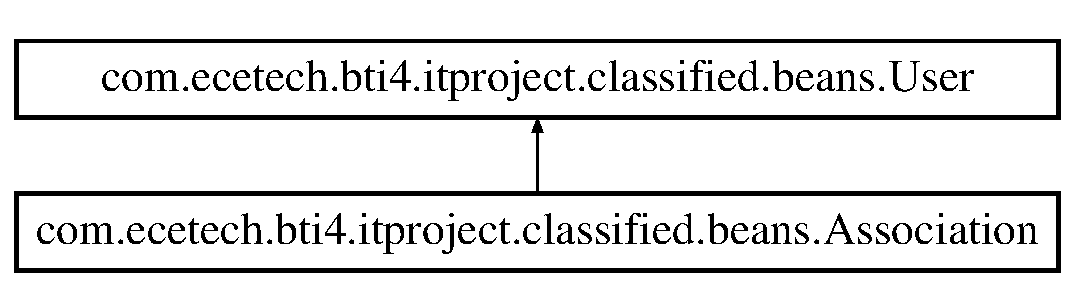
\includegraphics[height=2.000000cm]{classcom_1_1ecetech_1_1bti4_1_1itproject_1_1classified_1_1beans_1_1_association}
\end{center}
\end{figure}
\subsection*{Public Member Functions}
\begin{DoxyCompactItemize}
\item 
\hyperlink{classcom_1_1ecetech_1_1bti4_1_1itproject_1_1classified_1_1beans_1_1_association_a17d6f1725fe02b8e4534c9ecb04d8541}{Association} ()
\item 
\hyperlink{classcom_1_1ecetech_1_1bti4_1_1itproject_1_1classified_1_1beans_1_1_association_a064ee8543696e79afe38f33c2c967cfe}{Association} (String nom\+Ass, String siret\+Ass, int num\+Ad\+Ass, String rue\+Ad\+Ass, int cp\+Ad\+Ass, String ville\+Ad\+Ass, int tel\+Ass)
\item 
String \hyperlink{classcom_1_1ecetech_1_1bti4_1_1itproject_1_1classified_1_1beans_1_1_association_a2b6c89b2438c1914daeff46d61338cac}{get\+Nom\+Ass} ()
\item 
void \hyperlink{classcom_1_1ecetech_1_1bti4_1_1itproject_1_1classified_1_1beans_1_1_association_a882c3d46da0221ea90af71f1463cc2f4}{set\+Nom\+Ass} (String nom\+Ass)
\item 
String \hyperlink{classcom_1_1ecetech_1_1bti4_1_1itproject_1_1classified_1_1beans_1_1_association_a3d717b1c88eaf9a990d64f9ed436eebc}{get\+Siret\+Ass} ()
\item 
void \hyperlink{classcom_1_1ecetech_1_1bti4_1_1itproject_1_1classified_1_1beans_1_1_association_aab5103a1d73a114d348341ac0fce28c3}{set\+Siret\+Ass} (String siret\+Ass)
\item 
int \hyperlink{classcom_1_1ecetech_1_1bti4_1_1itproject_1_1classified_1_1beans_1_1_association_a28727ad9fc4568bb08a352d5d3109493}{get\+Num\+Ad\+Ass} ()
\item 
void \hyperlink{classcom_1_1ecetech_1_1bti4_1_1itproject_1_1classified_1_1beans_1_1_association_a4fb8d7006ef7adc7b86dcdf856365209}{set\+Num\+Ad\+Ass} (int num\+Ad\+Ass)
\item 
String \hyperlink{classcom_1_1ecetech_1_1bti4_1_1itproject_1_1classified_1_1beans_1_1_association_ad5dfa0d714b02e64f6a4babc844ccf95}{get\+Rue\+Ad\+Ass} ()
\item 
void \hyperlink{classcom_1_1ecetech_1_1bti4_1_1itproject_1_1classified_1_1beans_1_1_association_a20cf5b575f77131b065a3d9198b821d5}{set\+Rue\+Ad\+Ass} (String rue\+Ad\+Ass)
\item 
int \hyperlink{classcom_1_1ecetech_1_1bti4_1_1itproject_1_1classified_1_1beans_1_1_association_acc3d948f39a2ad79d9edaa784b9847e9}{get\+Cp\+Ad\+Ass} ()
\item 
void \hyperlink{classcom_1_1ecetech_1_1bti4_1_1itproject_1_1classified_1_1beans_1_1_association_a624a2f007c0b9797833e230ee6da34b8}{set\+Cp\+Ad\+Ass} (int cp\+Ad\+Ass)
\item 
String \hyperlink{classcom_1_1ecetech_1_1bti4_1_1itproject_1_1classified_1_1beans_1_1_association_ae0d00e261f53a29720c562e888e47fd7}{get\+Ville\+Ad\+Ass} ()
\item 
void \hyperlink{classcom_1_1ecetech_1_1bti4_1_1itproject_1_1classified_1_1beans_1_1_association_a36dcf28aea25ffa7a726aff15e88c9f9}{set\+Ville\+Ad\+Ass} (String ville\+Ad\+Ass)
\item 
int \hyperlink{classcom_1_1ecetech_1_1bti4_1_1itproject_1_1classified_1_1beans_1_1_association_a5e6da0b2bb1558b0425dfbe6691e22ea}{get\+Tel\+Ass} ()
\item 
void \hyperlink{classcom_1_1ecetech_1_1bti4_1_1itproject_1_1classified_1_1beans_1_1_association_aa3e7f8988163b0c7508f6eb4421bf64c}{set\+Tel\+Ass} (int tel\+Ass)
\item 
String \hyperlink{classcom_1_1ecetech_1_1bti4_1_1itproject_1_1classified_1_1beans_1_1_association_acd8b66ea9409c4c1752a6df35a0127df}{to\+String} ()
\end{DoxyCompactItemize}


\subsection{Constructor \& Destructor Documentation}
\index{com\+::ecetech\+::bti4\+::itproject\+::classified\+::beans\+::\+Association@{com\+::ecetech\+::bti4\+::itproject\+::classified\+::beans\+::\+Association}!Association@{Association}}
\index{Association@{Association}!com\+::ecetech\+::bti4\+::itproject\+::classified\+::beans\+::\+Association@{com\+::ecetech\+::bti4\+::itproject\+::classified\+::beans\+::\+Association}}
\subsubsection[{\texorpdfstring{Association()}{Association()}}]{\setlength{\rightskip}{0pt plus 5cm}com.\+ecetech.\+bti4.\+itproject.\+classified.\+beans.\+Association.\+Association (
\begin{DoxyParamCaption}
{}
\end{DoxyParamCaption}
)}\hypertarget{classcom_1_1ecetech_1_1bti4_1_1itproject_1_1classified_1_1beans_1_1_association_a17d6f1725fe02b8e4534c9ecb04d8541}{}\label{classcom_1_1ecetech_1_1bti4_1_1itproject_1_1classified_1_1beans_1_1_association_a17d6f1725fe02b8e4534c9ecb04d8541}
Constructeurs \index{com\+::ecetech\+::bti4\+::itproject\+::classified\+::beans\+::\+Association@{com\+::ecetech\+::bti4\+::itproject\+::classified\+::beans\+::\+Association}!Association@{Association}}
\index{Association@{Association}!com\+::ecetech\+::bti4\+::itproject\+::classified\+::beans\+::\+Association@{com\+::ecetech\+::bti4\+::itproject\+::classified\+::beans\+::\+Association}}
\subsubsection[{\texorpdfstring{Association(\+String nom\+Ass, String siret\+Ass, int num\+Ad\+Ass, String rue\+Ad\+Ass, int cp\+Ad\+Ass, String ville\+Ad\+Ass, int tel\+Ass)}{Association(String nomAss, String siretAss, int numAdAss, String rueAdAss, int cpAdAss, String villeAdAss, int telAss)}}]{\setlength{\rightskip}{0pt plus 5cm}com.\+ecetech.\+bti4.\+itproject.\+classified.\+beans.\+Association.\+Association (
\begin{DoxyParamCaption}
\item[{String}]{nom\+Ass, }
\item[{String}]{siret\+Ass, }
\item[{int}]{num\+Ad\+Ass, }
\item[{String}]{rue\+Ad\+Ass, }
\item[{int}]{cp\+Ad\+Ass, }
\item[{String}]{ville\+Ad\+Ass, }
\item[{int}]{tel\+Ass}
\end{DoxyParamCaption}
)}\hypertarget{classcom_1_1ecetech_1_1bti4_1_1itproject_1_1classified_1_1beans_1_1_association_a064ee8543696e79afe38f33c2c967cfe}{}\label{classcom_1_1ecetech_1_1bti4_1_1itproject_1_1classified_1_1beans_1_1_association_a064ee8543696e79afe38f33c2c967cfe}


\subsection{Member Function Documentation}
\index{com\+::ecetech\+::bti4\+::itproject\+::classified\+::beans\+::\+Association@{com\+::ecetech\+::bti4\+::itproject\+::classified\+::beans\+::\+Association}!get\+Cp\+Ad\+Ass@{get\+Cp\+Ad\+Ass}}
\index{get\+Cp\+Ad\+Ass@{get\+Cp\+Ad\+Ass}!com\+::ecetech\+::bti4\+::itproject\+::classified\+::beans\+::\+Association@{com\+::ecetech\+::bti4\+::itproject\+::classified\+::beans\+::\+Association}}
\subsubsection[{\texorpdfstring{get\+Cp\+Ad\+Ass()}{getCpAdAss()}}]{\setlength{\rightskip}{0pt plus 5cm}int com.\+ecetech.\+bti4.\+itproject.\+classified.\+beans.\+Association.\+get\+Cp\+Ad\+Ass (
\begin{DoxyParamCaption}
{}
\end{DoxyParamCaption}
)}\hypertarget{classcom_1_1ecetech_1_1bti4_1_1itproject_1_1classified_1_1beans_1_1_association_acc3d948f39a2ad79d9edaa784b9847e9}{}\label{classcom_1_1ecetech_1_1bti4_1_1itproject_1_1classified_1_1beans_1_1_association_acc3d948f39a2ad79d9edaa784b9847e9}
\index{com\+::ecetech\+::bti4\+::itproject\+::classified\+::beans\+::\+Association@{com\+::ecetech\+::bti4\+::itproject\+::classified\+::beans\+::\+Association}!get\+Nom\+Ass@{get\+Nom\+Ass}}
\index{get\+Nom\+Ass@{get\+Nom\+Ass}!com\+::ecetech\+::bti4\+::itproject\+::classified\+::beans\+::\+Association@{com\+::ecetech\+::bti4\+::itproject\+::classified\+::beans\+::\+Association}}
\subsubsection[{\texorpdfstring{get\+Nom\+Ass()}{getNomAss()}}]{\setlength{\rightskip}{0pt plus 5cm}String com.\+ecetech.\+bti4.\+itproject.\+classified.\+beans.\+Association.\+get\+Nom\+Ass (
\begin{DoxyParamCaption}
{}
\end{DoxyParamCaption}
)}\hypertarget{classcom_1_1ecetech_1_1bti4_1_1itproject_1_1classified_1_1beans_1_1_association_a2b6c89b2438c1914daeff46d61338cac}{}\label{classcom_1_1ecetech_1_1bti4_1_1itproject_1_1classified_1_1beans_1_1_association_a2b6c89b2438c1914daeff46d61338cac}
Getters \& Setters \index{com\+::ecetech\+::bti4\+::itproject\+::classified\+::beans\+::\+Association@{com\+::ecetech\+::bti4\+::itproject\+::classified\+::beans\+::\+Association}!get\+Num\+Ad\+Ass@{get\+Num\+Ad\+Ass}}
\index{get\+Num\+Ad\+Ass@{get\+Num\+Ad\+Ass}!com\+::ecetech\+::bti4\+::itproject\+::classified\+::beans\+::\+Association@{com\+::ecetech\+::bti4\+::itproject\+::classified\+::beans\+::\+Association}}
\subsubsection[{\texorpdfstring{get\+Num\+Ad\+Ass()}{getNumAdAss()}}]{\setlength{\rightskip}{0pt plus 5cm}int com.\+ecetech.\+bti4.\+itproject.\+classified.\+beans.\+Association.\+get\+Num\+Ad\+Ass (
\begin{DoxyParamCaption}
{}
\end{DoxyParamCaption}
)}\hypertarget{classcom_1_1ecetech_1_1bti4_1_1itproject_1_1classified_1_1beans_1_1_association_a28727ad9fc4568bb08a352d5d3109493}{}\label{classcom_1_1ecetech_1_1bti4_1_1itproject_1_1classified_1_1beans_1_1_association_a28727ad9fc4568bb08a352d5d3109493}
\index{com\+::ecetech\+::bti4\+::itproject\+::classified\+::beans\+::\+Association@{com\+::ecetech\+::bti4\+::itproject\+::classified\+::beans\+::\+Association}!get\+Rue\+Ad\+Ass@{get\+Rue\+Ad\+Ass}}
\index{get\+Rue\+Ad\+Ass@{get\+Rue\+Ad\+Ass}!com\+::ecetech\+::bti4\+::itproject\+::classified\+::beans\+::\+Association@{com\+::ecetech\+::bti4\+::itproject\+::classified\+::beans\+::\+Association}}
\subsubsection[{\texorpdfstring{get\+Rue\+Ad\+Ass()}{getRueAdAss()}}]{\setlength{\rightskip}{0pt plus 5cm}String com.\+ecetech.\+bti4.\+itproject.\+classified.\+beans.\+Association.\+get\+Rue\+Ad\+Ass (
\begin{DoxyParamCaption}
{}
\end{DoxyParamCaption}
)}\hypertarget{classcom_1_1ecetech_1_1bti4_1_1itproject_1_1classified_1_1beans_1_1_association_ad5dfa0d714b02e64f6a4babc844ccf95}{}\label{classcom_1_1ecetech_1_1bti4_1_1itproject_1_1classified_1_1beans_1_1_association_ad5dfa0d714b02e64f6a4babc844ccf95}
\index{com\+::ecetech\+::bti4\+::itproject\+::classified\+::beans\+::\+Association@{com\+::ecetech\+::bti4\+::itproject\+::classified\+::beans\+::\+Association}!get\+Siret\+Ass@{get\+Siret\+Ass}}
\index{get\+Siret\+Ass@{get\+Siret\+Ass}!com\+::ecetech\+::bti4\+::itproject\+::classified\+::beans\+::\+Association@{com\+::ecetech\+::bti4\+::itproject\+::classified\+::beans\+::\+Association}}
\subsubsection[{\texorpdfstring{get\+Siret\+Ass()}{getSiretAss()}}]{\setlength{\rightskip}{0pt plus 5cm}String com.\+ecetech.\+bti4.\+itproject.\+classified.\+beans.\+Association.\+get\+Siret\+Ass (
\begin{DoxyParamCaption}
{}
\end{DoxyParamCaption}
)}\hypertarget{classcom_1_1ecetech_1_1bti4_1_1itproject_1_1classified_1_1beans_1_1_association_a3d717b1c88eaf9a990d64f9ed436eebc}{}\label{classcom_1_1ecetech_1_1bti4_1_1itproject_1_1classified_1_1beans_1_1_association_a3d717b1c88eaf9a990d64f9ed436eebc}
\index{com\+::ecetech\+::bti4\+::itproject\+::classified\+::beans\+::\+Association@{com\+::ecetech\+::bti4\+::itproject\+::classified\+::beans\+::\+Association}!get\+Tel\+Ass@{get\+Tel\+Ass}}
\index{get\+Tel\+Ass@{get\+Tel\+Ass}!com\+::ecetech\+::bti4\+::itproject\+::classified\+::beans\+::\+Association@{com\+::ecetech\+::bti4\+::itproject\+::classified\+::beans\+::\+Association}}
\subsubsection[{\texorpdfstring{get\+Tel\+Ass()}{getTelAss()}}]{\setlength{\rightskip}{0pt plus 5cm}int com.\+ecetech.\+bti4.\+itproject.\+classified.\+beans.\+Association.\+get\+Tel\+Ass (
\begin{DoxyParamCaption}
{}
\end{DoxyParamCaption}
)}\hypertarget{classcom_1_1ecetech_1_1bti4_1_1itproject_1_1classified_1_1beans_1_1_association_a5e6da0b2bb1558b0425dfbe6691e22ea}{}\label{classcom_1_1ecetech_1_1bti4_1_1itproject_1_1classified_1_1beans_1_1_association_a5e6da0b2bb1558b0425dfbe6691e22ea}
\index{com\+::ecetech\+::bti4\+::itproject\+::classified\+::beans\+::\+Association@{com\+::ecetech\+::bti4\+::itproject\+::classified\+::beans\+::\+Association}!get\+Ville\+Ad\+Ass@{get\+Ville\+Ad\+Ass}}
\index{get\+Ville\+Ad\+Ass@{get\+Ville\+Ad\+Ass}!com\+::ecetech\+::bti4\+::itproject\+::classified\+::beans\+::\+Association@{com\+::ecetech\+::bti4\+::itproject\+::classified\+::beans\+::\+Association}}
\subsubsection[{\texorpdfstring{get\+Ville\+Ad\+Ass()}{getVilleAdAss()}}]{\setlength{\rightskip}{0pt plus 5cm}String com.\+ecetech.\+bti4.\+itproject.\+classified.\+beans.\+Association.\+get\+Ville\+Ad\+Ass (
\begin{DoxyParamCaption}
{}
\end{DoxyParamCaption}
)}\hypertarget{classcom_1_1ecetech_1_1bti4_1_1itproject_1_1classified_1_1beans_1_1_association_ae0d00e261f53a29720c562e888e47fd7}{}\label{classcom_1_1ecetech_1_1bti4_1_1itproject_1_1classified_1_1beans_1_1_association_ae0d00e261f53a29720c562e888e47fd7}
\index{com\+::ecetech\+::bti4\+::itproject\+::classified\+::beans\+::\+Association@{com\+::ecetech\+::bti4\+::itproject\+::classified\+::beans\+::\+Association}!set\+Cp\+Ad\+Ass@{set\+Cp\+Ad\+Ass}}
\index{set\+Cp\+Ad\+Ass@{set\+Cp\+Ad\+Ass}!com\+::ecetech\+::bti4\+::itproject\+::classified\+::beans\+::\+Association@{com\+::ecetech\+::bti4\+::itproject\+::classified\+::beans\+::\+Association}}
\subsubsection[{\texorpdfstring{set\+Cp\+Ad\+Ass(int cp\+Ad\+Ass)}{setCpAdAss(int cpAdAss)}}]{\setlength{\rightskip}{0pt plus 5cm}void com.\+ecetech.\+bti4.\+itproject.\+classified.\+beans.\+Association.\+set\+Cp\+Ad\+Ass (
\begin{DoxyParamCaption}
\item[{int}]{cp\+Ad\+Ass}
\end{DoxyParamCaption}
)}\hypertarget{classcom_1_1ecetech_1_1bti4_1_1itproject_1_1classified_1_1beans_1_1_association_a624a2f007c0b9797833e230ee6da34b8}{}\label{classcom_1_1ecetech_1_1bti4_1_1itproject_1_1classified_1_1beans_1_1_association_a624a2f007c0b9797833e230ee6da34b8}
\index{com\+::ecetech\+::bti4\+::itproject\+::classified\+::beans\+::\+Association@{com\+::ecetech\+::bti4\+::itproject\+::classified\+::beans\+::\+Association}!set\+Nom\+Ass@{set\+Nom\+Ass}}
\index{set\+Nom\+Ass@{set\+Nom\+Ass}!com\+::ecetech\+::bti4\+::itproject\+::classified\+::beans\+::\+Association@{com\+::ecetech\+::bti4\+::itproject\+::classified\+::beans\+::\+Association}}
\subsubsection[{\texorpdfstring{set\+Nom\+Ass(\+String nom\+Ass)}{setNomAss(String nomAss)}}]{\setlength{\rightskip}{0pt plus 5cm}void com.\+ecetech.\+bti4.\+itproject.\+classified.\+beans.\+Association.\+set\+Nom\+Ass (
\begin{DoxyParamCaption}
\item[{String}]{nom\+Ass}
\end{DoxyParamCaption}
)}\hypertarget{classcom_1_1ecetech_1_1bti4_1_1itproject_1_1classified_1_1beans_1_1_association_a882c3d46da0221ea90af71f1463cc2f4}{}\label{classcom_1_1ecetech_1_1bti4_1_1itproject_1_1classified_1_1beans_1_1_association_a882c3d46da0221ea90af71f1463cc2f4}
\index{com\+::ecetech\+::bti4\+::itproject\+::classified\+::beans\+::\+Association@{com\+::ecetech\+::bti4\+::itproject\+::classified\+::beans\+::\+Association}!set\+Num\+Ad\+Ass@{set\+Num\+Ad\+Ass}}
\index{set\+Num\+Ad\+Ass@{set\+Num\+Ad\+Ass}!com\+::ecetech\+::bti4\+::itproject\+::classified\+::beans\+::\+Association@{com\+::ecetech\+::bti4\+::itproject\+::classified\+::beans\+::\+Association}}
\subsubsection[{\texorpdfstring{set\+Num\+Ad\+Ass(int num\+Ad\+Ass)}{setNumAdAss(int numAdAss)}}]{\setlength{\rightskip}{0pt plus 5cm}void com.\+ecetech.\+bti4.\+itproject.\+classified.\+beans.\+Association.\+set\+Num\+Ad\+Ass (
\begin{DoxyParamCaption}
\item[{int}]{num\+Ad\+Ass}
\end{DoxyParamCaption}
)}\hypertarget{classcom_1_1ecetech_1_1bti4_1_1itproject_1_1classified_1_1beans_1_1_association_a4fb8d7006ef7adc7b86dcdf856365209}{}\label{classcom_1_1ecetech_1_1bti4_1_1itproject_1_1classified_1_1beans_1_1_association_a4fb8d7006ef7adc7b86dcdf856365209}
\index{com\+::ecetech\+::bti4\+::itproject\+::classified\+::beans\+::\+Association@{com\+::ecetech\+::bti4\+::itproject\+::classified\+::beans\+::\+Association}!set\+Rue\+Ad\+Ass@{set\+Rue\+Ad\+Ass}}
\index{set\+Rue\+Ad\+Ass@{set\+Rue\+Ad\+Ass}!com\+::ecetech\+::bti4\+::itproject\+::classified\+::beans\+::\+Association@{com\+::ecetech\+::bti4\+::itproject\+::classified\+::beans\+::\+Association}}
\subsubsection[{\texorpdfstring{set\+Rue\+Ad\+Ass(\+String rue\+Ad\+Ass)}{setRueAdAss(String rueAdAss)}}]{\setlength{\rightskip}{0pt plus 5cm}void com.\+ecetech.\+bti4.\+itproject.\+classified.\+beans.\+Association.\+set\+Rue\+Ad\+Ass (
\begin{DoxyParamCaption}
\item[{String}]{rue\+Ad\+Ass}
\end{DoxyParamCaption}
)}\hypertarget{classcom_1_1ecetech_1_1bti4_1_1itproject_1_1classified_1_1beans_1_1_association_a20cf5b575f77131b065a3d9198b821d5}{}\label{classcom_1_1ecetech_1_1bti4_1_1itproject_1_1classified_1_1beans_1_1_association_a20cf5b575f77131b065a3d9198b821d5}
\index{com\+::ecetech\+::bti4\+::itproject\+::classified\+::beans\+::\+Association@{com\+::ecetech\+::bti4\+::itproject\+::classified\+::beans\+::\+Association}!set\+Siret\+Ass@{set\+Siret\+Ass}}
\index{set\+Siret\+Ass@{set\+Siret\+Ass}!com\+::ecetech\+::bti4\+::itproject\+::classified\+::beans\+::\+Association@{com\+::ecetech\+::bti4\+::itproject\+::classified\+::beans\+::\+Association}}
\subsubsection[{\texorpdfstring{set\+Siret\+Ass(\+String siret\+Ass)}{setSiretAss(String siretAss)}}]{\setlength{\rightskip}{0pt plus 5cm}void com.\+ecetech.\+bti4.\+itproject.\+classified.\+beans.\+Association.\+set\+Siret\+Ass (
\begin{DoxyParamCaption}
\item[{String}]{siret\+Ass}
\end{DoxyParamCaption}
)}\hypertarget{classcom_1_1ecetech_1_1bti4_1_1itproject_1_1classified_1_1beans_1_1_association_aab5103a1d73a114d348341ac0fce28c3}{}\label{classcom_1_1ecetech_1_1bti4_1_1itproject_1_1classified_1_1beans_1_1_association_aab5103a1d73a114d348341ac0fce28c3}
\index{com\+::ecetech\+::bti4\+::itproject\+::classified\+::beans\+::\+Association@{com\+::ecetech\+::bti4\+::itproject\+::classified\+::beans\+::\+Association}!set\+Tel\+Ass@{set\+Tel\+Ass}}
\index{set\+Tel\+Ass@{set\+Tel\+Ass}!com\+::ecetech\+::bti4\+::itproject\+::classified\+::beans\+::\+Association@{com\+::ecetech\+::bti4\+::itproject\+::classified\+::beans\+::\+Association}}
\subsubsection[{\texorpdfstring{set\+Tel\+Ass(int tel\+Ass)}{setTelAss(int telAss)}}]{\setlength{\rightskip}{0pt plus 5cm}void com.\+ecetech.\+bti4.\+itproject.\+classified.\+beans.\+Association.\+set\+Tel\+Ass (
\begin{DoxyParamCaption}
\item[{int}]{tel\+Ass}
\end{DoxyParamCaption}
)}\hypertarget{classcom_1_1ecetech_1_1bti4_1_1itproject_1_1classified_1_1beans_1_1_association_aa3e7f8988163b0c7508f6eb4421bf64c}{}\label{classcom_1_1ecetech_1_1bti4_1_1itproject_1_1classified_1_1beans_1_1_association_aa3e7f8988163b0c7508f6eb4421bf64c}
\index{com\+::ecetech\+::bti4\+::itproject\+::classified\+::beans\+::\+Association@{com\+::ecetech\+::bti4\+::itproject\+::classified\+::beans\+::\+Association}!set\+Ville\+Ad\+Ass@{set\+Ville\+Ad\+Ass}}
\index{set\+Ville\+Ad\+Ass@{set\+Ville\+Ad\+Ass}!com\+::ecetech\+::bti4\+::itproject\+::classified\+::beans\+::\+Association@{com\+::ecetech\+::bti4\+::itproject\+::classified\+::beans\+::\+Association}}
\subsubsection[{\texorpdfstring{set\+Ville\+Ad\+Ass(\+String ville\+Ad\+Ass)}{setVilleAdAss(String villeAdAss)}}]{\setlength{\rightskip}{0pt plus 5cm}void com.\+ecetech.\+bti4.\+itproject.\+classified.\+beans.\+Association.\+set\+Ville\+Ad\+Ass (
\begin{DoxyParamCaption}
\item[{String}]{ville\+Ad\+Ass}
\end{DoxyParamCaption}
)}\hypertarget{classcom_1_1ecetech_1_1bti4_1_1itproject_1_1classified_1_1beans_1_1_association_a36dcf28aea25ffa7a726aff15e88c9f9}{}\label{classcom_1_1ecetech_1_1bti4_1_1itproject_1_1classified_1_1beans_1_1_association_a36dcf28aea25ffa7a726aff15e88c9f9}
\index{com\+::ecetech\+::bti4\+::itproject\+::classified\+::beans\+::\+Association@{com\+::ecetech\+::bti4\+::itproject\+::classified\+::beans\+::\+Association}!to\+String@{to\+String}}
\index{to\+String@{to\+String}!com\+::ecetech\+::bti4\+::itproject\+::classified\+::beans\+::\+Association@{com\+::ecetech\+::bti4\+::itproject\+::classified\+::beans\+::\+Association}}
\subsubsection[{\texorpdfstring{to\+String()}{toString()}}]{\setlength{\rightskip}{0pt plus 5cm}String com.\+ecetech.\+bti4.\+itproject.\+classified.\+beans.\+Association.\+to\+String (
\begin{DoxyParamCaption}
{}
\end{DoxyParamCaption}
)}\hypertarget{classcom_1_1ecetech_1_1bti4_1_1itproject_1_1classified_1_1beans_1_1_association_acd8b66ea9409c4c1752a6df35a0127df}{}\label{classcom_1_1ecetech_1_1bti4_1_1itproject_1_1classified_1_1beans_1_1_association_acd8b66ea9409c4c1752a6df35a0127df}


The documentation for this class was generated from the following file\+:\begin{DoxyCompactItemize}
\item 
Classified-\/\+Model/src/com/ecetech/bti4/itproject/classified/beans/\hyperlink{_association_8java}{Association.\+java}\end{DoxyCompactItemize}

\hypertarget{classcom_1_1ecetech_1_1bti4_1_1itproject_1_1classified_1_1dao_1_1_association_d_a_o}{}\section{com.\+ecetech.\+bti4.\+itproject.\+classified.\+dao.\+Association\+D\+AO Class Reference}
\label{classcom_1_1ecetech_1_1bti4_1_1itproject_1_1classified_1_1dao_1_1_association_d_a_o}\index{com.\+ecetech.\+bti4.\+itproject.\+classified.\+dao.\+Association\+D\+AO@{com.\+ecetech.\+bti4.\+itproject.\+classified.\+dao.\+Association\+D\+AO}}
\subsection*{Static Public Member Functions}
\begin{DoxyCompactItemize}
\item 
static \hyperlink{classcom_1_1ecetech_1_1bti4_1_1itproject_1_1classified_1_1beans_1_1_association}{Association} \hyperlink{classcom_1_1ecetech_1_1bti4_1_1itproject_1_1classified_1_1dao_1_1_association_d_a_o_aa162d952d94f0879a9610d9dd94b9326}{get\+Asso\+User} (String id\+User)  throws S\+Q\+L\+Exception 
\item 
static void \hyperlink{classcom_1_1ecetech_1_1bti4_1_1itproject_1_1classified_1_1dao_1_1_association_d_a_o_a36927ba0db8b58b9a413d9b41a29d585}{add\+Asso\+User} (String Mail\+User, String Mdp\+User, String Permission\+User, String Nom\+Ass, String Siret\+Ass, int Num\+Ad\+Ass, String Rue\+Ad\+Ass, int Cp\+Ad\+Ass, String Ville\+Ad\+Ass, int Tel\+Ass)  throws S\+Q\+L\+Exception 
\item 
static void \hyperlink{classcom_1_1ecetech_1_1bti4_1_1itproject_1_1classified_1_1dao_1_1_association_d_a_o_a38507a0fc15499fabbcd9ce9f74da511}{delete\+Asso\+User} (String id\+User)  throws S\+Q\+L\+Exception 
\item 
static void \hyperlink{classcom_1_1ecetech_1_1bti4_1_1itproject_1_1classified_1_1dao_1_1_association_d_a_o_a27417f3e5267a2d65e0849faf7652a52}{update\+Nom\+Asso} (String id\+User, String nom\+Asso)  throws S\+Q\+L\+Exception 
\item 
static void \hyperlink{classcom_1_1ecetech_1_1bti4_1_1itproject_1_1classified_1_1dao_1_1_association_d_a_o_a1821ad5594c12b3ac543a7cc64b8f815}{update\+Num\+Ad\+Asso} (String id\+User, int num\+Ad\+Asso)  throws S\+Q\+L\+Exception 
\item 
static void \hyperlink{classcom_1_1ecetech_1_1bti4_1_1itproject_1_1classified_1_1dao_1_1_association_d_a_o_adf30b71b8932d9cd78eb649826de61d5}{update\+Rue\+Ad\+Asso} (String id\+User, String rue\+Ad\+Asso)  throws S\+Q\+L\+Exception 
\item 
static void \hyperlink{classcom_1_1ecetech_1_1bti4_1_1itproject_1_1classified_1_1dao_1_1_association_d_a_o_a7c9c96fcfb5e950d61f79df851f9575b}{update\+Cp\+Ad\+Asso} (String id\+User, int cp\+Ad\+Asso)  throws S\+Q\+L\+Exception 
\item 
static void \hyperlink{classcom_1_1ecetech_1_1bti4_1_1itproject_1_1classified_1_1dao_1_1_association_d_a_o_a65048bf95fdcd35ee35d5c0bee623b8b}{update\+Ville\+Ad\+Asso} (String id\+User, String Ville\+Ad\+Asso)  throws S\+Q\+L\+Exception 
\item 
static void \hyperlink{classcom_1_1ecetech_1_1bti4_1_1itproject_1_1classified_1_1dao_1_1_association_d_a_o_a4714a27c39d0537a449cc3f47cf9e737}{update\+Tel\+Asso} (String id\+User, int Tel\+Asso)  throws S\+Q\+L\+Exception 
\end{DoxyCompactItemize}


\subsection{Detailed Description}
Represente une association \begin{DoxyAuthor}{Author}
Maeva, Adrien, Moaz 
\end{DoxyAuthor}


\subsection{Member Function Documentation}
\index{com\+::ecetech\+::bti4\+::itproject\+::classified\+::dao\+::\+Association\+D\+AO@{com\+::ecetech\+::bti4\+::itproject\+::classified\+::dao\+::\+Association\+D\+AO}!add\+Asso\+User@{add\+Asso\+User}}
\index{add\+Asso\+User@{add\+Asso\+User}!com\+::ecetech\+::bti4\+::itproject\+::classified\+::dao\+::\+Association\+D\+AO@{com\+::ecetech\+::bti4\+::itproject\+::classified\+::dao\+::\+Association\+D\+AO}}
\subsubsection[{\texorpdfstring{add\+Asso\+User(\+String Mail\+User, String Mdp\+User, String Permission\+User, String Nom\+Ass, String Siret\+Ass, int Num\+Ad\+Ass, String Rue\+Ad\+Ass, int Cp\+Ad\+Ass, String Ville\+Ad\+Ass, int Tel\+Ass)}{addAssoUser(String MailUser, String MdpUser, String PermissionUser, String NomAss, String SiretAss, int NumAdAss, String RueAdAss, int CpAdAss, String VilleAdAss, int TelAss)}}]{\setlength{\rightskip}{0pt plus 5cm}static void com.\+ecetech.\+bti4.\+itproject.\+classified.\+dao.\+Association\+D\+A\+O.\+add\+Asso\+User (
\begin{DoxyParamCaption}
\item[{String}]{Mail\+User, }
\item[{String}]{Mdp\+User, }
\item[{String}]{Permission\+User, }
\item[{String}]{Nom\+Ass, }
\item[{String}]{Siret\+Ass, }
\item[{int}]{Num\+Ad\+Ass, }
\item[{String}]{Rue\+Ad\+Ass, }
\item[{int}]{Cp\+Ad\+Ass, }
\item[{String}]{Ville\+Ad\+Ass, }
\item[{int}]{Tel\+Ass}
\end{DoxyParamCaption}
) throws S\+Q\+L\+Exception\hspace{0.3cm}{\ttfamily [static]}}\hypertarget{classcom_1_1ecetech_1_1bti4_1_1itproject_1_1classified_1_1dao_1_1_association_d_a_o_a36927ba0db8b58b9a413d9b41a29d585}{}\label{classcom_1_1ecetech_1_1bti4_1_1itproject_1_1classified_1_1dao_1_1_association_d_a_o_a36927ba0db8b58b9a413d9b41a29d585}
public fonction \hyperlink{classcom_1_1ecetech_1_1bti4_1_1itproject_1_1classified_1_1dao_1_1_association_d_a_o_a36927ba0db8b58b9a413d9b41a29d585}{add\+Asso\+User()}  Ajoute une association a la base de donnee

Ne renvoie rien \index{com\+::ecetech\+::bti4\+::itproject\+::classified\+::dao\+::\+Association\+D\+AO@{com\+::ecetech\+::bti4\+::itproject\+::classified\+::dao\+::\+Association\+D\+AO}!delete\+Asso\+User@{delete\+Asso\+User}}
\index{delete\+Asso\+User@{delete\+Asso\+User}!com\+::ecetech\+::bti4\+::itproject\+::classified\+::dao\+::\+Association\+D\+AO@{com\+::ecetech\+::bti4\+::itproject\+::classified\+::dao\+::\+Association\+D\+AO}}
\subsubsection[{\texorpdfstring{delete\+Asso\+User(\+String id\+User)}{deleteAssoUser(String idUser)}}]{\setlength{\rightskip}{0pt plus 5cm}static void com.\+ecetech.\+bti4.\+itproject.\+classified.\+dao.\+Association\+D\+A\+O.\+delete\+Asso\+User (
\begin{DoxyParamCaption}
\item[{String}]{id\+User}
\end{DoxyParamCaption}
) throws S\+Q\+L\+Exception\hspace{0.3cm}{\ttfamily [static]}}\hypertarget{classcom_1_1ecetech_1_1bti4_1_1itproject_1_1classified_1_1dao_1_1_association_d_a_o_a38507a0fc15499fabbcd9ce9f74da511}{}\label{classcom_1_1ecetech_1_1bti4_1_1itproject_1_1classified_1_1dao_1_1_association_d_a_o_a38507a0fc15499fabbcd9ce9f74da511}
public fonction \hyperlink{classcom_1_1ecetech_1_1bti4_1_1itproject_1_1classified_1_1dao_1_1_association_d_a_o_a38507a0fc15499fabbcd9ce9f74da511}{delete\+Asso\+User()}  Supprime une association de la base de donnee

Ne renvoie rien \index{com\+::ecetech\+::bti4\+::itproject\+::classified\+::dao\+::\+Association\+D\+AO@{com\+::ecetech\+::bti4\+::itproject\+::classified\+::dao\+::\+Association\+D\+AO}!get\+Asso\+User@{get\+Asso\+User}}
\index{get\+Asso\+User@{get\+Asso\+User}!com\+::ecetech\+::bti4\+::itproject\+::classified\+::dao\+::\+Association\+D\+AO@{com\+::ecetech\+::bti4\+::itproject\+::classified\+::dao\+::\+Association\+D\+AO}}
\subsubsection[{\texorpdfstring{get\+Asso\+User(\+String id\+User)}{getAssoUser(String idUser)}}]{\setlength{\rightskip}{0pt plus 5cm}static {\bf Association} com.\+ecetech.\+bti4.\+itproject.\+classified.\+dao.\+Association\+D\+A\+O.\+get\+Asso\+User (
\begin{DoxyParamCaption}
\item[{String}]{id\+User}
\end{DoxyParamCaption}
) throws S\+Q\+L\+Exception\hspace{0.3cm}{\ttfamily [static]}}\hypertarget{classcom_1_1ecetech_1_1bti4_1_1itproject_1_1classified_1_1dao_1_1_association_d_a_o_aa162d952d94f0879a9610d9dd94b9326}{}\label{classcom_1_1ecetech_1_1bti4_1_1itproject_1_1classified_1_1dao_1_1_association_d_a_o_aa162d952d94f0879a9610d9dd94b9326}
public fonction \hyperlink{classcom_1_1ecetech_1_1bti4_1_1itproject_1_1classified_1_1dao_1_1_association_d_a_o_aa162d952d94f0879a9610d9dd94b9326}{get\+Asso\+User()}  Affiche une association

Renvoie une Arraylist contenant une association de la base de donnee \index{com\+::ecetech\+::bti4\+::itproject\+::classified\+::dao\+::\+Association\+D\+AO@{com\+::ecetech\+::bti4\+::itproject\+::classified\+::dao\+::\+Association\+D\+AO}!update\+Cp\+Ad\+Asso@{update\+Cp\+Ad\+Asso}}
\index{update\+Cp\+Ad\+Asso@{update\+Cp\+Ad\+Asso}!com\+::ecetech\+::bti4\+::itproject\+::classified\+::dao\+::\+Association\+D\+AO@{com\+::ecetech\+::bti4\+::itproject\+::classified\+::dao\+::\+Association\+D\+AO}}
\subsubsection[{\texorpdfstring{update\+Cp\+Ad\+Asso(\+String id\+User, int cp\+Ad\+Asso)}{updateCpAdAsso(String idUser, int cpAdAsso)}}]{\setlength{\rightskip}{0pt plus 5cm}static void com.\+ecetech.\+bti4.\+itproject.\+classified.\+dao.\+Association\+D\+A\+O.\+update\+Cp\+Ad\+Asso (
\begin{DoxyParamCaption}
\item[{String}]{id\+User, }
\item[{int}]{cp\+Ad\+Asso}
\end{DoxyParamCaption}
) throws S\+Q\+L\+Exception\hspace{0.3cm}{\ttfamily [static]}}\hypertarget{classcom_1_1ecetech_1_1bti4_1_1itproject_1_1classified_1_1dao_1_1_association_d_a_o_a7c9c96fcfb5e950d61f79df851f9575b}{}\label{classcom_1_1ecetech_1_1bti4_1_1itproject_1_1classified_1_1dao_1_1_association_d_a_o_a7c9c96fcfb5e950d61f79df851f9575b}
public fonction update\+Cp\+Assor()  Modifie le numero d\textquotesingle{}une association de la base de donnee

Ne renvoie rien \index{com\+::ecetech\+::bti4\+::itproject\+::classified\+::dao\+::\+Association\+D\+AO@{com\+::ecetech\+::bti4\+::itproject\+::classified\+::dao\+::\+Association\+D\+AO}!update\+Nom\+Asso@{update\+Nom\+Asso}}
\index{update\+Nom\+Asso@{update\+Nom\+Asso}!com\+::ecetech\+::bti4\+::itproject\+::classified\+::dao\+::\+Association\+D\+AO@{com\+::ecetech\+::bti4\+::itproject\+::classified\+::dao\+::\+Association\+D\+AO}}
\subsubsection[{\texorpdfstring{update\+Nom\+Asso(\+String id\+User, String nom\+Asso)}{updateNomAsso(String idUser, String nomAsso)}}]{\setlength{\rightskip}{0pt plus 5cm}static void com.\+ecetech.\+bti4.\+itproject.\+classified.\+dao.\+Association\+D\+A\+O.\+update\+Nom\+Asso (
\begin{DoxyParamCaption}
\item[{String}]{id\+User, }
\item[{String}]{nom\+Asso}
\end{DoxyParamCaption}
) throws S\+Q\+L\+Exception\hspace{0.3cm}{\ttfamily [static]}}\hypertarget{classcom_1_1ecetech_1_1bti4_1_1itproject_1_1classified_1_1dao_1_1_association_d_a_o_a27417f3e5267a2d65e0849faf7652a52}{}\label{classcom_1_1ecetech_1_1bti4_1_1itproject_1_1classified_1_1dao_1_1_association_d_a_o_a27417f3e5267a2d65e0849faf7652a52}
public fonction update\+Nom\+Asso\+Asso()  Modifie le nom d\textquotesingle{}une association

Ne renvoie rien \index{com\+::ecetech\+::bti4\+::itproject\+::classified\+::dao\+::\+Association\+D\+AO@{com\+::ecetech\+::bti4\+::itproject\+::classified\+::dao\+::\+Association\+D\+AO}!update\+Num\+Ad\+Asso@{update\+Num\+Ad\+Asso}}
\index{update\+Num\+Ad\+Asso@{update\+Num\+Ad\+Asso}!com\+::ecetech\+::bti4\+::itproject\+::classified\+::dao\+::\+Association\+D\+AO@{com\+::ecetech\+::bti4\+::itproject\+::classified\+::dao\+::\+Association\+D\+AO}}
\subsubsection[{\texorpdfstring{update\+Num\+Ad\+Asso(\+String id\+User, int num\+Ad\+Asso)}{updateNumAdAsso(String idUser, int numAdAsso)}}]{\setlength{\rightskip}{0pt plus 5cm}static void com.\+ecetech.\+bti4.\+itproject.\+classified.\+dao.\+Association\+D\+A\+O.\+update\+Num\+Ad\+Asso (
\begin{DoxyParamCaption}
\item[{String}]{id\+User, }
\item[{int}]{num\+Ad\+Asso}
\end{DoxyParamCaption}
) throws S\+Q\+L\+Exception\hspace{0.3cm}{\ttfamily [static]}}\hypertarget{classcom_1_1ecetech_1_1bti4_1_1itproject_1_1classified_1_1dao_1_1_association_d_a_o_a1821ad5594c12b3ac543a7cc64b8f815}{}\label{classcom_1_1ecetech_1_1bti4_1_1itproject_1_1classified_1_1dao_1_1_association_d_a_o_a1821ad5594c12b3ac543a7cc64b8f815}
public fonction update\+Num\+Asso()  Modifie le numero d\textquotesingle{}une association de la base de donnee

Ne renvoie rien \index{com\+::ecetech\+::bti4\+::itproject\+::classified\+::dao\+::\+Association\+D\+AO@{com\+::ecetech\+::bti4\+::itproject\+::classified\+::dao\+::\+Association\+D\+AO}!update\+Rue\+Ad\+Asso@{update\+Rue\+Ad\+Asso}}
\index{update\+Rue\+Ad\+Asso@{update\+Rue\+Ad\+Asso}!com\+::ecetech\+::bti4\+::itproject\+::classified\+::dao\+::\+Association\+D\+AO@{com\+::ecetech\+::bti4\+::itproject\+::classified\+::dao\+::\+Association\+D\+AO}}
\subsubsection[{\texorpdfstring{update\+Rue\+Ad\+Asso(\+String id\+User, String rue\+Ad\+Asso)}{updateRueAdAsso(String idUser, String rueAdAsso)}}]{\setlength{\rightskip}{0pt plus 5cm}static void com.\+ecetech.\+bti4.\+itproject.\+classified.\+dao.\+Association\+D\+A\+O.\+update\+Rue\+Ad\+Asso (
\begin{DoxyParamCaption}
\item[{String}]{id\+User, }
\item[{String}]{rue\+Ad\+Asso}
\end{DoxyParamCaption}
) throws S\+Q\+L\+Exception\hspace{0.3cm}{\ttfamily [static]}}\hypertarget{classcom_1_1ecetech_1_1bti4_1_1itproject_1_1classified_1_1dao_1_1_association_d_a_o_adf30b71b8932d9cd78eb649826de61d5}{}\label{classcom_1_1ecetech_1_1bti4_1_1itproject_1_1classified_1_1dao_1_1_association_d_a_o_adf30b71b8932d9cd78eb649826de61d5}
public fonction update\+Rue\+Asso()  Modifie la rue d\textquotesingle{}une association de la base de donnee

Ne renvoie rien \index{com\+::ecetech\+::bti4\+::itproject\+::classified\+::dao\+::\+Association\+D\+AO@{com\+::ecetech\+::bti4\+::itproject\+::classified\+::dao\+::\+Association\+D\+AO}!update\+Tel\+Asso@{update\+Tel\+Asso}}
\index{update\+Tel\+Asso@{update\+Tel\+Asso}!com\+::ecetech\+::bti4\+::itproject\+::classified\+::dao\+::\+Association\+D\+AO@{com\+::ecetech\+::bti4\+::itproject\+::classified\+::dao\+::\+Association\+D\+AO}}
\subsubsection[{\texorpdfstring{update\+Tel\+Asso(\+String id\+User, int Tel\+Asso)}{updateTelAsso(String idUser, int TelAsso)}}]{\setlength{\rightskip}{0pt plus 5cm}static void com.\+ecetech.\+bti4.\+itproject.\+classified.\+dao.\+Association\+D\+A\+O.\+update\+Tel\+Asso (
\begin{DoxyParamCaption}
\item[{String}]{id\+User, }
\item[{int}]{Tel\+Asso}
\end{DoxyParamCaption}
) throws S\+Q\+L\+Exception\hspace{0.3cm}{\ttfamily [static]}}\hypertarget{classcom_1_1ecetech_1_1bti4_1_1itproject_1_1classified_1_1dao_1_1_association_d_a_o_a4714a27c39d0537a449cc3f47cf9e737}{}\label{classcom_1_1ecetech_1_1bti4_1_1itproject_1_1classified_1_1dao_1_1_association_d_a_o_a4714a27c39d0537a449cc3f47cf9e737}
public fonction \hyperlink{classcom_1_1ecetech_1_1bti4_1_1itproject_1_1classified_1_1dao_1_1_association_d_a_o_a4714a27c39d0537a449cc3f47cf9e737}{update\+Tel\+Asso()}  Modifie le numero de telephone d\textquotesingle{}une association de la base de donnee

Ne renvoie rien \index{com\+::ecetech\+::bti4\+::itproject\+::classified\+::dao\+::\+Association\+D\+AO@{com\+::ecetech\+::bti4\+::itproject\+::classified\+::dao\+::\+Association\+D\+AO}!update\+Ville\+Ad\+Asso@{update\+Ville\+Ad\+Asso}}
\index{update\+Ville\+Ad\+Asso@{update\+Ville\+Ad\+Asso}!com\+::ecetech\+::bti4\+::itproject\+::classified\+::dao\+::\+Association\+D\+AO@{com\+::ecetech\+::bti4\+::itproject\+::classified\+::dao\+::\+Association\+D\+AO}}
\subsubsection[{\texorpdfstring{update\+Ville\+Ad\+Asso(\+String id\+User, String Ville\+Ad\+Asso)}{updateVilleAdAsso(String idUser, String VilleAdAsso)}}]{\setlength{\rightskip}{0pt plus 5cm}static void com.\+ecetech.\+bti4.\+itproject.\+classified.\+dao.\+Association\+D\+A\+O.\+update\+Ville\+Ad\+Asso (
\begin{DoxyParamCaption}
\item[{String}]{id\+User, }
\item[{String}]{Ville\+Ad\+Asso}
\end{DoxyParamCaption}
) throws S\+Q\+L\+Exception\hspace{0.3cm}{\ttfamily [static]}}\hypertarget{classcom_1_1ecetech_1_1bti4_1_1itproject_1_1classified_1_1dao_1_1_association_d_a_o_a65048bf95fdcd35ee35d5c0bee623b8b}{}\label{classcom_1_1ecetech_1_1bti4_1_1itproject_1_1classified_1_1dao_1_1_association_d_a_o_a65048bf95fdcd35ee35d5c0bee623b8b}
public fonction \hyperlink{classcom_1_1ecetech_1_1bti4_1_1itproject_1_1classified_1_1dao_1_1_association_d_a_o_a65048bf95fdcd35ee35d5c0bee623b8b}{update\+Ville\+Ad\+Asso()}  Modifie la ville d\textquotesingle{}une association de la base de donnee

Ne renvoie rien 

The documentation for this class was generated from the following file\+:\begin{DoxyCompactItemize}
\item 
src/com/ecetech/bti4/itproject/classified/dao/Association\+D\+A\+O.\+java\end{DoxyCompactItemize}

\hypertarget{classcom_1_1ecetech_1_1bti4_1_1itproject_1_1classified_1_1beans_1_1_categorie}{}\section{com.\+ecetech.\+bti4.\+itproject.\+classified.\+beans.\+Categorie Class Reference}
\label{classcom_1_1ecetech_1_1bti4_1_1itproject_1_1classified_1_1beans_1_1_categorie}\index{com.\+ecetech.\+bti4.\+itproject.\+classified.\+beans.\+Categorie@{com.\+ecetech.\+bti4.\+itproject.\+classified.\+beans.\+Categorie}}
\subsection*{Public Member Functions}
\begin{DoxyCompactItemize}
\item 
\hyperlink{classcom_1_1ecetech_1_1bti4_1_1itproject_1_1classified_1_1beans_1_1_categorie_a151c5e769ad87b8b5cf882e9d5b6b8d6}{Categorie} (int id\+Categorie, String nom\+Categorie, int id\+Type)
\item 
int \hyperlink{classcom_1_1ecetech_1_1bti4_1_1itproject_1_1classified_1_1beans_1_1_categorie_a70d771b7a2c6d24807b4ad8a7599dfb3}{get\+Id\+Categorie} ()
\item 
void {\bfseries set\+Id\+Categorie} (int id\+Categorie)\hypertarget{classcom_1_1ecetech_1_1bti4_1_1itproject_1_1classified_1_1beans_1_1_categorie_a7cfebd4ed0c6170eb8eb7e629d667d64}{}\label{classcom_1_1ecetech_1_1bti4_1_1itproject_1_1classified_1_1beans_1_1_categorie_a7cfebd4ed0c6170eb8eb7e629d667d64}

\item 
String {\bfseries get\+Nom\+Categorie} ()\hypertarget{classcom_1_1ecetech_1_1bti4_1_1itproject_1_1classified_1_1beans_1_1_categorie_a5f5d43367d9964e07a45492c036fe49f}{}\label{classcom_1_1ecetech_1_1bti4_1_1itproject_1_1classified_1_1beans_1_1_categorie_a5f5d43367d9964e07a45492c036fe49f}

\item 
void {\bfseries set\+Nom\+Categorie} (String nom\+Categorie)\hypertarget{classcom_1_1ecetech_1_1bti4_1_1itproject_1_1classified_1_1beans_1_1_categorie_aece9e65b0b2001cde88cdc99ad00206b}{}\label{classcom_1_1ecetech_1_1bti4_1_1itproject_1_1classified_1_1beans_1_1_categorie_aece9e65b0b2001cde88cdc99ad00206b}

\item 
int {\bfseries get\+Id\+Type} ()\hypertarget{classcom_1_1ecetech_1_1bti4_1_1itproject_1_1classified_1_1beans_1_1_categorie_a75d6febe1021333b087a7e98e764e053}{}\label{classcom_1_1ecetech_1_1bti4_1_1itproject_1_1classified_1_1beans_1_1_categorie_a75d6febe1021333b087a7e98e764e053}

\item 
void {\bfseries set\+Id\+Type} (int id\+Type)\hypertarget{classcom_1_1ecetech_1_1bti4_1_1itproject_1_1classified_1_1beans_1_1_categorie_a4a978c04d124319a8fcee08d529352a1}{}\label{classcom_1_1ecetech_1_1bti4_1_1itproject_1_1classified_1_1beans_1_1_categorie_a4a978c04d124319a8fcee08d529352a1}

\item 
String {\bfseries to\+String} ()\hypertarget{classcom_1_1ecetech_1_1bti4_1_1itproject_1_1classified_1_1beans_1_1_categorie_ab5a1c587aa78c348fd1c894754133050}{}\label{classcom_1_1ecetech_1_1bti4_1_1itproject_1_1classified_1_1beans_1_1_categorie_ab5a1c587aa78c348fd1c894754133050}

\end{DoxyCompactItemize}


\subsection{Detailed Description}
Represente une catégorie \begin{DoxyAuthor}{Author}
Maeva, Adrien, Moaz 
\end{DoxyAuthor}


\subsection{Constructor \& Destructor Documentation}
\index{com\+::ecetech\+::bti4\+::itproject\+::classified\+::beans\+::\+Categorie@{com\+::ecetech\+::bti4\+::itproject\+::classified\+::beans\+::\+Categorie}!Categorie@{Categorie}}
\index{Categorie@{Categorie}!com\+::ecetech\+::bti4\+::itproject\+::classified\+::beans\+::\+Categorie@{com\+::ecetech\+::bti4\+::itproject\+::classified\+::beans\+::\+Categorie}}
\subsubsection[{\texorpdfstring{Categorie(int id\+Categorie, String nom\+Categorie, int id\+Type)}{Categorie(int idCategorie, String nomCategorie, int idType)}}]{\setlength{\rightskip}{0pt plus 5cm}com.\+ecetech.\+bti4.\+itproject.\+classified.\+beans.\+Categorie.\+Categorie (
\begin{DoxyParamCaption}
\item[{int}]{id\+Categorie, }
\item[{String}]{nom\+Categorie, }
\item[{int}]{id\+Type}
\end{DoxyParamCaption}
)}\hypertarget{classcom_1_1ecetech_1_1bti4_1_1itproject_1_1classified_1_1beans_1_1_categorie_a151c5e769ad87b8b5cf882e9d5b6b8d6}{}\label{classcom_1_1ecetech_1_1bti4_1_1itproject_1_1classified_1_1beans_1_1_categorie_a151c5e769ad87b8b5cf882e9d5b6b8d6}
Constructor


\begin{DoxyParams}{Parameters}
{\em id\+Categorie} & \\
\hline
{\em nom\+Categorie} & \\
\hline
{\em id\+Type} & \\
\hline
\end{DoxyParams}


\subsection{Member Function Documentation}
\index{com\+::ecetech\+::bti4\+::itproject\+::classified\+::beans\+::\+Categorie@{com\+::ecetech\+::bti4\+::itproject\+::classified\+::beans\+::\+Categorie}!get\+Id\+Categorie@{get\+Id\+Categorie}}
\index{get\+Id\+Categorie@{get\+Id\+Categorie}!com\+::ecetech\+::bti4\+::itproject\+::classified\+::beans\+::\+Categorie@{com\+::ecetech\+::bti4\+::itproject\+::classified\+::beans\+::\+Categorie}}
\subsubsection[{\texorpdfstring{get\+Id\+Categorie()}{getIdCategorie()}}]{\setlength{\rightskip}{0pt plus 5cm}int com.\+ecetech.\+bti4.\+itproject.\+classified.\+beans.\+Categorie.\+get\+Id\+Categorie (
\begin{DoxyParamCaption}
{}
\end{DoxyParamCaption}
)}\hypertarget{classcom_1_1ecetech_1_1bti4_1_1itproject_1_1classified_1_1beans_1_1_categorie_a70d771b7a2c6d24807b4ad8a7599dfb3}{}\label{classcom_1_1ecetech_1_1bti4_1_1itproject_1_1classified_1_1beans_1_1_categorie_a70d771b7a2c6d24807b4ad8a7599dfb3}
Getters and setters

\begin{DoxyReturn}{Returns}

\end{DoxyReturn}


The documentation for this class was generated from the following file\+:\begin{DoxyCompactItemize}
\item 
src/com/ecetech/bti4/itproject/classified/beans/Categorie.\+java\end{DoxyCompactItemize}

\hypertarget{classcom_1_1ecetech_1_1bti4_1_1itproject_1_1classified_1_1dao_1_1_categorie_d_a_o}{}\section{com.\+ecetech.\+bti4.\+itproject.\+classified.\+dao.\+Categorie\+D\+AO Class Reference}
\label{classcom_1_1ecetech_1_1bti4_1_1itproject_1_1classified_1_1dao_1_1_categorie_d_a_o}\index{com.\+ecetech.\+bti4.\+itproject.\+classified.\+dao.\+Categorie\+D\+AO@{com.\+ecetech.\+bti4.\+itproject.\+classified.\+dao.\+Categorie\+D\+AO}}
\subsection*{Static Public Member Functions}
\begin{DoxyCompactItemize}
\item 
static Array\+List$<$ \hyperlink{classcom_1_1ecetech_1_1bti4_1_1itproject_1_1classified_1_1beans_1_1_categorie}{Categorie} $>$ \hyperlink{classcom_1_1ecetech_1_1bti4_1_1itproject_1_1classified_1_1dao_1_1_categorie_d_a_o_a3e7fe47e89b6a9fc25fd8037d3f5acf7}{get\+All\+Cat} ()
\item 
static boolean \hyperlink{classcom_1_1ecetech_1_1bti4_1_1itproject_1_1classified_1_1dao_1_1_categorie_d_a_o_a003d6a6dce5a0c96895c78547931a5ca}{change\+Cat} (\hyperlink{classcom_1_1ecetech_1_1bti4_1_1itproject_1_1classified_1_1beans_1_1_categorie}{Categorie} categorie)
\end{DoxyCompactItemize}


\subsection{Member Function Documentation}
\index{com\+::ecetech\+::bti4\+::itproject\+::classified\+::dao\+::\+Categorie\+D\+AO@{com\+::ecetech\+::bti4\+::itproject\+::classified\+::dao\+::\+Categorie\+D\+AO}!change\+Cat@{change\+Cat}}
\index{change\+Cat@{change\+Cat}!com\+::ecetech\+::bti4\+::itproject\+::classified\+::dao\+::\+Categorie\+D\+AO@{com\+::ecetech\+::bti4\+::itproject\+::classified\+::dao\+::\+Categorie\+D\+AO}}
\subsubsection[{\texorpdfstring{change\+Cat(\+Categorie categorie)}{changeCat(Categorie categorie)}}]{\setlength{\rightskip}{0pt plus 5cm}static boolean com.\+ecetech.\+bti4.\+itproject.\+classified.\+dao.\+Categorie\+D\+A\+O.\+change\+Cat (
\begin{DoxyParamCaption}
\item[{{\bf Categorie}}]{categorie}
\end{DoxyParamCaption}
)\hspace{0.3cm}{\ttfamily [static]}}\hypertarget{classcom_1_1ecetech_1_1bti4_1_1itproject_1_1classified_1_1dao_1_1_categorie_d_a_o_a003d6a6dce5a0c96895c78547931a5ca}{}\label{classcom_1_1ecetech_1_1bti4_1_1itproject_1_1classified_1_1dao_1_1_categorie_d_a_o_a003d6a6dce5a0c96895c78547931a5ca}
\index{com\+::ecetech\+::bti4\+::itproject\+::classified\+::dao\+::\+Categorie\+D\+AO@{com\+::ecetech\+::bti4\+::itproject\+::classified\+::dao\+::\+Categorie\+D\+AO}!get\+All\+Cat@{get\+All\+Cat}}
\index{get\+All\+Cat@{get\+All\+Cat}!com\+::ecetech\+::bti4\+::itproject\+::classified\+::dao\+::\+Categorie\+D\+AO@{com\+::ecetech\+::bti4\+::itproject\+::classified\+::dao\+::\+Categorie\+D\+AO}}
\subsubsection[{\texorpdfstring{get\+All\+Cat()}{getAllCat()}}]{\setlength{\rightskip}{0pt plus 5cm}static Array\+List$<${\bf Categorie}$>$ com.\+ecetech.\+bti4.\+itproject.\+classified.\+dao.\+Categorie\+D\+A\+O.\+get\+All\+Cat (
\begin{DoxyParamCaption}
{}
\end{DoxyParamCaption}
)\hspace{0.3cm}{\ttfamily [static]}}\hypertarget{classcom_1_1ecetech_1_1bti4_1_1itproject_1_1classified_1_1dao_1_1_categorie_d_a_o_a3e7fe47e89b6a9fc25fd8037d3f5acf7}{}\label{classcom_1_1ecetech_1_1bti4_1_1itproject_1_1classified_1_1dao_1_1_categorie_d_a_o_a3e7fe47e89b6a9fc25fd8037d3f5acf7}


The documentation for this class was generated from the following file\+:\begin{DoxyCompactItemize}
\item 
Classified-\/\+Model/src/com/ecetech/bti4/itproject/classified/dao/\hyperlink{_categorie_d_a_o_8java}{Categorie\+D\+A\+O.\+java}\end{DoxyCompactItemize}

\hypertarget{classcom_1_1ecetech_1_1bti4_1_1itproject_1_1classified_1_1common_1_1_d_b_action}{}\section{com.\+ecetech.\+bti4.\+itproject.\+classified.\+common.\+D\+B\+Action Class Reference}
\label{classcom_1_1ecetech_1_1bti4_1_1itproject_1_1classified_1_1common_1_1_d_b_action}\index{com.\+ecetech.\+bti4.\+itproject.\+classified.\+common.\+D\+B\+Action@{com.\+ecetech.\+bti4.\+itproject.\+classified.\+common.\+D\+B\+Action}}
\subsection*{Static Public Member Functions}
\begin{DoxyCompactItemize}
\item 
static Exception \hyperlink{classcom_1_1ecetech_1_1bti4_1_1itproject_1_1classified_1_1common_1_1_d_b_action_a03b522e1388500132c0de54ad5ba35da}{D\+B\+Connexion} ()
\item 
static int \hyperlink{classcom_1_1ecetech_1_1bti4_1_1itproject_1_1classified_1_1common_1_1_d_b_action_a9e2f615b938168702c83370c13f629ad}{D\+B\+Close} ()
\item 
static Connection \hyperlink{classcom_1_1ecetech_1_1bti4_1_1itproject_1_1classified_1_1common_1_1_d_b_action_a5831883b0b490e9528f2604904610dbe}{get\+Con} ()
\item 
static void {\bfseries set\+Con} (Connection con)\hypertarget{classcom_1_1ecetech_1_1bti4_1_1itproject_1_1classified_1_1common_1_1_d_b_action_a1229309e09cf59bc09814488e449608e}{}\label{classcom_1_1ecetech_1_1bti4_1_1itproject_1_1classified_1_1common_1_1_d_b_action_a1229309e09cf59bc09814488e449608e}

\item 
static Statement {\bfseries get\+Stm} ()\hypertarget{classcom_1_1ecetech_1_1bti4_1_1itproject_1_1classified_1_1common_1_1_d_b_action_acbac8f8d13d537ed7be8553809762134}{}\label{classcom_1_1ecetech_1_1bti4_1_1itproject_1_1classified_1_1common_1_1_d_b_action_acbac8f8d13d537ed7be8553809762134}

\item 
static void {\bfseries set\+Stm} (Statement stm)\hypertarget{classcom_1_1ecetech_1_1bti4_1_1itproject_1_1classified_1_1common_1_1_d_b_action_a6aedd826db70e9c3736ca969599c1d43}{}\label{classcom_1_1ecetech_1_1bti4_1_1itproject_1_1classified_1_1common_1_1_d_b_action_a6aedd826db70e9c3736ca969599c1d43}

\item 
static Result\+Set {\bfseries get\+Res} ()\hypertarget{classcom_1_1ecetech_1_1bti4_1_1itproject_1_1classified_1_1common_1_1_d_b_action_ae8cb329cdf28bc94217b723b422491be}{}\label{classcom_1_1ecetech_1_1bti4_1_1itproject_1_1classified_1_1common_1_1_d_b_action_ae8cb329cdf28bc94217b723b422491be}

\item 
static void {\bfseries set\+Res} (Result\+Set res)\hypertarget{classcom_1_1ecetech_1_1bti4_1_1itproject_1_1classified_1_1common_1_1_d_b_action_a86c0a551394ed96766b38cd4117d49f4}{}\label{classcom_1_1ecetech_1_1bti4_1_1itproject_1_1classified_1_1common_1_1_d_b_action_a86c0a551394ed96766b38cd4117d49f4}

\end{DoxyCompactItemize}


\subsection{Detailed Description}
Class DB Action, methodes liée a la base de donnée \begin{DoxyAuthor}{Author}
Maeva, Adrien, Moaz 
\end{DoxyAuthor}


\subsection{Member Function Documentation}
\index{com\+::ecetech\+::bti4\+::itproject\+::classified\+::common\+::\+D\+B\+Action@{com\+::ecetech\+::bti4\+::itproject\+::classified\+::common\+::\+D\+B\+Action}!D\+B\+Close@{D\+B\+Close}}
\index{D\+B\+Close@{D\+B\+Close}!com\+::ecetech\+::bti4\+::itproject\+::classified\+::common\+::\+D\+B\+Action@{com\+::ecetech\+::bti4\+::itproject\+::classified\+::common\+::\+D\+B\+Action}}
\subsubsection[{\texorpdfstring{D\+B\+Close()}{DBClose()}}]{\setlength{\rightskip}{0pt plus 5cm}static int com.\+ecetech.\+bti4.\+itproject.\+classified.\+common.\+D\+B\+Action.\+D\+B\+Close (
\begin{DoxyParamCaption}
{}
\end{DoxyParamCaption}
)\hspace{0.3cm}{\ttfamily [static]}}\hypertarget{classcom_1_1ecetech_1_1bti4_1_1itproject_1_1classified_1_1common_1_1_d_b_action_a9e2f615b938168702c83370c13f629ad}{}\label{classcom_1_1ecetech_1_1bti4_1_1itproject_1_1classified_1_1common_1_1_d_b_action_a9e2f615b938168702c83370c13f629ad}
public static \hyperlink{classcom_1_1ecetech_1_1bti4_1_1itproject_1_1classified_1_1common_1_1_d_b_action_a9e2f615b938168702c83370c13f629ad}{D\+B\+Close()} termine la connection a la base de donnee \begin{DoxyReturn}{Returns}
un message d\textquotesingle{}erreur si besoins 
\end{DoxyReturn}
\index{com\+::ecetech\+::bti4\+::itproject\+::classified\+::common\+::\+D\+B\+Action@{com\+::ecetech\+::bti4\+::itproject\+::classified\+::common\+::\+D\+B\+Action}!D\+B\+Connexion@{D\+B\+Connexion}}
\index{D\+B\+Connexion@{D\+B\+Connexion}!com\+::ecetech\+::bti4\+::itproject\+::classified\+::common\+::\+D\+B\+Action@{com\+::ecetech\+::bti4\+::itproject\+::classified\+::common\+::\+D\+B\+Action}}
\subsubsection[{\texorpdfstring{D\+B\+Connexion()}{DBConnexion()}}]{\setlength{\rightskip}{0pt plus 5cm}static Exception com.\+ecetech.\+bti4.\+itproject.\+classified.\+common.\+D\+B\+Action.\+D\+B\+Connexion (
\begin{DoxyParamCaption}
{}
\end{DoxyParamCaption}
)\hspace{0.3cm}{\ttfamily [static]}}\hypertarget{classcom_1_1ecetech_1_1bti4_1_1itproject_1_1classified_1_1common_1_1_d_b_action_a03b522e1388500132c0de54ad5ba35da}{}\label{classcom_1_1ecetech_1_1bti4_1_1itproject_1_1classified_1_1common_1_1_d_b_action_a03b522e1388500132c0de54ad5ba35da}
public static \hyperlink{classcom_1_1ecetech_1_1bti4_1_1itproject_1_1classified_1_1common_1_1_d_b_action_a03b522e1388500132c0de54ad5ba35da}{D\+B\+Connexion()} initie une connection a la base de donnee \begin{DoxyReturn}{Returns}
null si connecte ou un message d\textquotesingle{}erreur 
\end{DoxyReturn}
\index{com\+::ecetech\+::bti4\+::itproject\+::classified\+::common\+::\+D\+B\+Action@{com\+::ecetech\+::bti4\+::itproject\+::classified\+::common\+::\+D\+B\+Action}!get\+Con@{get\+Con}}
\index{get\+Con@{get\+Con}!com\+::ecetech\+::bti4\+::itproject\+::classified\+::common\+::\+D\+B\+Action@{com\+::ecetech\+::bti4\+::itproject\+::classified\+::common\+::\+D\+B\+Action}}
\subsubsection[{\texorpdfstring{get\+Con()}{getCon()}}]{\setlength{\rightskip}{0pt plus 5cm}static Connection com.\+ecetech.\+bti4.\+itproject.\+classified.\+common.\+D\+B\+Action.\+get\+Con (
\begin{DoxyParamCaption}
{}
\end{DoxyParamCaption}
)\hspace{0.3cm}{\ttfamily [static]}}\hypertarget{classcom_1_1ecetech_1_1bti4_1_1itproject_1_1classified_1_1common_1_1_d_b_action_a5831883b0b490e9528f2604904610dbe}{}\label{classcom_1_1ecetech_1_1bti4_1_1itproject_1_1classified_1_1common_1_1_d_b_action_a5831883b0b490e9528f2604904610dbe}
Getters \& setters

\begin{DoxyReturn}{Returns}

\end{DoxyReturn}


The documentation for this class was generated from the following file\+:\begin{DoxyCompactItemize}
\item 
src/com/ecetech/bti4/itproject/classified/common/D\+B\+Action.\+java\end{DoxyCompactItemize}

\hypertarget{classcom_1_1ecetech_1_1bti4_1_1itproject_1_1classified_1_1beans_1_1_entreprise}{}\section{com.\+ecetech.\+bti4.\+itproject.\+classified.\+beans.\+Entreprise Class Reference}
\label{classcom_1_1ecetech_1_1bti4_1_1itproject_1_1classified_1_1beans_1_1_entreprise}\index{com.\+ecetech.\+bti4.\+itproject.\+classified.\+beans.\+Entreprise@{com.\+ecetech.\+bti4.\+itproject.\+classified.\+beans.\+Entreprise}}
Inheritance diagram for com.\+ecetech.\+bti4.\+itproject.\+classified.\+beans.\+Entreprise\+:\begin{figure}[H]
\begin{center}
\leavevmode
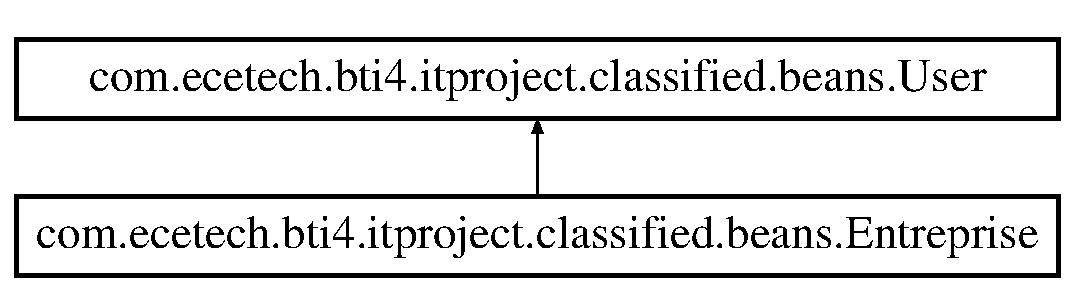
\includegraphics[height=2.000000cm]{classcom_1_1ecetech_1_1bti4_1_1itproject_1_1classified_1_1beans_1_1_entreprise}
\end{center}
\end{figure}
\subsection*{Public Member Functions}
\begin{DoxyCompactItemize}
\item 
\hyperlink{classcom_1_1ecetech_1_1bti4_1_1itproject_1_1classified_1_1beans_1_1_entreprise_aefa560c8cbc49291fc3b6edeb2ba3698}{Entreprise} ()
\item 
\hyperlink{classcom_1_1ecetech_1_1bti4_1_1itproject_1_1classified_1_1beans_1_1_entreprise_a3ec943cd404efd0740de5a4b09f52931}{Entreprise} (String nom\+\_\+\+Ent, int num\+\_\+\+Ad\+\_\+\+Ent, String rue\+\_\+\+Ad\+\_\+\+Ent, int cp\+\_\+\+Ad\+\_\+\+Ent, String ville\+\_\+\+Ad\+\_\+\+Ent, int tel\+\_\+\+Ent, String siren\+\_\+\+Ent)
\item 
String \hyperlink{classcom_1_1ecetech_1_1bti4_1_1itproject_1_1classified_1_1beans_1_1_entreprise_af37b8b9efaaf7632684f37480bf9f44e}{get\+Nom\+\_\+\+Ent} ()
\item 
void \hyperlink{classcom_1_1ecetech_1_1bti4_1_1itproject_1_1classified_1_1beans_1_1_entreprise_a9e7b76bd675dcc0512eda1b920e2eae9}{set\+Nom\+\_\+\+Ent} (String nom\+\_\+\+Ent)
\item 
int \hyperlink{classcom_1_1ecetech_1_1bti4_1_1itproject_1_1classified_1_1beans_1_1_entreprise_a309a59d49cf4d85a64befcc4b95db1d2}{get\+Num\+\_\+\+Ad\+\_\+\+Ent} ()
\item 
void \hyperlink{classcom_1_1ecetech_1_1bti4_1_1itproject_1_1classified_1_1beans_1_1_entreprise_a7ffd79c4d0fc8b0e6337e0b71785d0ef}{set\+Num\+\_\+\+Ad\+\_\+\+Ent} (int num\+\_\+\+Ad\+\_\+\+Ent)
\item 
String \hyperlink{classcom_1_1ecetech_1_1bti4_1_1itproject_1_1classified_1_1beans_1_1_entreprise_a418160f37dc6e11378c3d1e4a1e45fb7}{get\+Rue\+\_\+\+Ad\+\_\+\+Ent} ()
\item 
void \hyperlink{classcom_1_1ecetech_1_1bti4_1_1itproject_1_1classified_1_1beans_1_1_entreprise_a69c7107244fa65f7e68b6720e7c9f7e6}{set\+Rue\+\_\+\+Ad\+\_\+\+Ent} (String rue\+\_\+\+Ad\+\_\+\+Ent)
\item 
int \hyperlink{classcom_1_1ecetech_1_1bti4_1_1itproject_1_1classified_1_1beans_1_1_entreprise_ac938eb585f0d23a10c47dbc6a76cd119}{get\+Cp\+\_\+\+Ad\+\_\+\+Ent} ()
\item 
void \hyperlink{classcom_1_1ecetech_1_1bti4_1_1itproject_1_1classified_1_1beans_1_1_entreprise_a6860ae9e5faa4a1adc75f05bb50feec1}{set\+Cp\+\_\+\+Ad\+\_\+\+Ent} (int cp\+\_\+\+Ad\+\_\+\+Ent)
\item 
String \hyperlink{classcom_1_1ecetech_1_1bti4_1_1itproject_1_1classified_1_1beans_1_1_entreprise_a0724ddfa83a6a0acabe2d4bc588b26cd}{get\+Ville\+\_\+\+Ad\+\_\+\+Ent} ()
\item 
void \hyperlink{classcom_1_1ecetech_1_1bti4_1_1itproject_1_1classified_1_1beans_1_1_entreprise_afd0bef50f48a3adddf52cfec54d667ab}{set\+Ville\+\_\+\+Ad\+\_\+\+Ent} (String ville\+\_\+\+Ad\+\_\+\+Ent)
\item 
int \hyperlink{classcom_1_1ecetech_1_1bti4_1_1itproject_1_1classified_1_1beans_1_1_entreprise_aef6cb67c4b543ca6301cbf91eaf64ad2}{get\+Tel\+\_\+\+Ent} ()
\item 
void \hyperlink{classcom_1_1ecetech_1_1bti4_1_1itproject_1_1classified_1_1beans_1_1_entreprise_a70d04874668bd2ffff5689fd2cd91938}{set\+Tel\+\_\+\+Ent} (int tel\+\_\+\+Ent)
\item 
String \hyperlink{classcom_1_1ecetech_1_1bti4_1_1itproject_1_1classified_1_1beans_1_1_entreprise_ac46b48fd3e1136b88ede50bb957a4f79}{get\+Siren\+\_\+\+Ent} ()
\item 
void \hyperlink{classcom_1_1ecetech_1_1bti4_1_1itproject_1_1classified_1_1beans_1_1_entreprise_a87ede27dc581965c4c12436b07692bd2}{set\+Siren\+\_\+\+Ent} (String siren\+\_\+\+Ent)
\item 
String \hyperlink{classcom_1_1ecetech_1_1bti4_1_1itproject_1_1classified_1_1beans_1_1_entreprise_a7a8adc9f3c5b1d83613168d1aff3e6db}{to\+String} ()
\end{DoxyCompactItemize}


\subsection{Constructor \& Destructor Documentation}
\index{com\+::ecetech\+::bti4\+::itproject\+::classified\+::beans\+::\+Entreprise@{com\+::ecetech\+::bti4\+::itproject\+::classified\+::beans\+::\+Entreprise}!Entreprise@{Entreprise}}
\index{Entreprise@{Entreprise}!com\+::ecetech\+::bti4\+::itproject\+::classified\+::beans\+::\+Entreprise@{com\+::ecetech\+::bti4\+::itproject\+::classified\+::beans\+::\+Entreprise}}
\subsubsection[{\texorpdfstring{Entreprise()}{Entreprise()}}]{\setlength{\rightskip}{0pt plus 5cm}com.\+ecetech.\+bti4.\+itproject.\+classified.\+beans.\+Entreprise.\+Entreprise (
\begin{DoxyParamCaption}
{}
\end{DoxyParamCaption}
)}\hypertarget{classcom_1_1ecetech_1_1bti4_1_1itproject_1_1classified_1_1beans_1_1_entreprise_aefa560c8cbc49291fc3b6edeb2ba3698}{}\label{classcom_1_1ecetech_1_1bti4_1_1itproject_1_1classified_1_1beans_1_1_entreprise_aefa560c8cbc49291fc3b6edeb2ba3698}
\index{com\+::ecetech\+::bti4\+::itproject\+::classified\+::beans\+::\+Entreprise@{com\+::ecetech\+::bti4\+::itproject\+::classified\+::beans\+::\+Entreprise}!Entreprise@{Entreprise}}
\index{Entreprise@{Entreprise}!com\+::ecetech\+::bti4\+::itproject\+::classified\+::beans\+::\+Entreprise@{com\+::ecetech\+::bti4\+::itproject\+::classified\+::beans\+::\+Entreprise}}
\subsubsection[{\texorpdfstring{Entreprise(\+String nom\+\_\+\+Ent, int num\+\_\+\+Ad\+\_\+\+Ent, String rue\+\_\+\+Ad\+\_\+\+Ent, int cp\+\_\+\+Ad\+\_\+\+Ent, String ville\+\_\+\+Ad\+\_\+\+Ent, int tel\+\_\+\+Ent, String siren\+\_\+\+Ent)}{Entreprise(String nom_Ent, int num_Ad_Ent, String rue_Ad_Ent, int cp_Ad_Ent, String ville_Ad_Ent, int tel_Ent, String siren_Ent)}}]{\setlength{\rightskip}{0pt plus 5cm}com.\+ecetech.\+bti4.\+itproject.\+classified.\+beans.\+Entreprise.\+Entreprise (
\begin{DoxyParamCaption}
\item[{String}]{nom\+\_\+\+Ent, }
\item[{int}]{num\+\_\+\+Ad\+\_\+\+Ent, }
\item[{String}]{rue\+\_\+\+Ad\+\_\+\+Ent, }
\item[{int}]{cp\+\_\+\+Ad\+\_\+\+Ent, }
\item[{String}]{ville\+\_\+\+Ad\+\_\+\+Ent, }
\item[{int}]{tel\+\_\+\+Ent, }
\item[{String}]{siren\+\_\+\+Ent}
\end{DoxyParamCaption}
)}\hypertarget{classcom_1_1ecetech_1_1bti4_1_1itproject_1_1classified_1_1beans_1_1_entreprise_a3ec943cd404efd0740de5a4b09f52931}{}\label{classcom_1_1ecetech_1_1bti4_1_1itproject_1_1classified_1_1beans_1_1_entreprise_a3ec943cd404efd0740de5a4b09f52931}


\subsection{Member Function Documentation}
\index{com\+::ecetech\+::bti4\+::itproject\+::classified\+::beans\+::\+Entreprise@{com\+::ecetech\+::bti4\+::itproject\+::classified\+::beans\+::\+Entreprise}!get\+Cp\+\_\+\+Ad\+\_\+\+Ent@{get\+Cp\+\_\+\+Ad\+\_\+\+Ent}}
\index{get\+Cp\+\_\+\+Ad\+\_\+\+Ent@{get\+Cp\+\_\+\+Ad\+\_\+\+Ent}!com\+::ecetech\+::bti4\+::itproject\+::classified\+::beans\+::\+Entreprise@{com\+::ecetech\+::bti4\+::itproject\+::classified\+::beans\+::\+Entreprise}}
\subsubsection[{\texorpdfstring{get\+Cp\+\_\+\+Ad\+\_\+\+Ent()}{getCp_Ad_Ent()}}]{\setlength{\rightskip}{0pt plus 5cm}int com.\+ecetech.\+bti4.\+itproject.\+classified.\+beans.\+Entreprise.\+get\+Cp\+\_\+\+Ad\+\_\+\+Ent (
\begin{DoxyParamCaption}
{}
\end{DoxyParamCaption}
)}\hypertarget{classcom_1_1ecetech_1_1bti4_1_1itproject_1_1classified_1_1beans_1_1_entreprise_ac938eb585f0d23a10c47dbc6a76cd119}{}\label{classcom_1_1ecetech_1_1bti4_1_1itproject_1_1classified_1_1beans_1_1_entreprise_ac938eb585f0d23a10c47dbc6a76cd119}
\index{com\+::ecetech\+::bti4\+::itproject\+::classified\+::beans\+::\+Entreprise@{com\+::ecetech\+::bti4\+::itproject\+::classified\+::beans\+::\+Entreprise}!get\+Nom\+\_\+\+Ent@{get\+Nom\+\_\+\+Ent}}
\index{get\+Nom\+\_\+\+Ent@{get\+Nom\+\_\+\+Ent}!com\+::ecetech\+::bti4\+::itproject\+::classified\+::beans\+::\+Entreprise@{com\+::ecetech\+::bti4\+::itproject\+::classified\+::beans\+::\+Entreprise}}
\subsubsection[{\texorpdfstring{get\+Nom\+\_\+\+Ent()}{getNom_Ent()}}]{\setlength{\rightskip}{0pt plus 5cm}String com.\+ecetech.\+bti4.\+itproject.\+classified.\+beans.\+Entreprise.\+get\+Nom\+\_\+\+Ent (
\begin{DoxyParamCaption}
{}
\end{DoxyParamCaption}
)}\hypertarget{classcom_1_1ecetech_1_1bti4_1_1itproject_1_1classified_1_1beans_1_1_entreprise_af37b8b9efaaf7632684f37480bf9f44e}{}\label{classcom_1_1ecetech_1_1bti4_1_1itproject_1_1classified_1_1beans_1_1_entreprise_af37b8b9efaaf7632684f37480bf9f44e}
\index{com\+::ecetech\+::bti4\+::itproject\+::classified\+::beans\+::\+Entreprise@{com\+::ecetech\+::bti4\+::itproject\+::classified\+::beans\+::\+Entreprise}!get\+Num\+\_\+\+Ad\+\_\+\+Ent@{get\+Num\+\_\+\+Ad\+\_\+\+Ent}}
\index{get\+Num\+\_\+\+Ad\+\_\+\+Ent@{get\+Num\+\_\+\+Ad\+\_\+\+Ent}!com\+::ecetech\+::bti4\+::itproject\+::classified\+::beans\+::\+Entreprise@{com\+::ecetech\+::bti4\+::itproject\+::classified\+::beans\+::\+Entreprise}}
\subsubsection[{\texorpdfstring{get\+Num\+\_\+\+Ad\+\_\+\+Ent()}{getNum_Ad_Ent()}}]{\setlength{\rightskip}{0pt plus 5cm}int com.\+ecetech.\+bti4.\+itproject.\+classified.\+beans.\+Entreprise.\+get\+Num\+\_\+\+Ad\+\_\+\+Ent (
\begin{DoxyParamCaption}
{}
\end{DoxyParamCaption}
)}\hypertarget{classcom_1_1ecetech_1_1bti4_1_1itproject_1_1classified_1_1beans_1_1_entreprise_a309a59d49cf4d85a64befcc4b95db1d2}{}\label{classcom_1_1ecetech_1_1bti4_1_1itproject_1_1classified_1_1beans_1_1_entreprise_a309a59d49cf4d85a64befcc4b95db1d2}
\index{com\+::ecetech\+::bti4\+::itproject\+::classified\+::beans\+::\+Entreprise@{com\+::ecetech\+::bti4\+::itproject\+::classified\+::beans\+::\+Entreprise}!get\+Rue\+\_\+\+Ad\+\_\+\+Ent@{get\+Rue\+\_\+\+Ad\+\_\+\+Ent}}
\index{get\+Rue\+\_\+\+Ad\+\_\+\+Ent@{get\+Rue\+\_\+\+Ad\+\_\+\+Ent}!com\+::ecetech\+::bti4\+::itproject\+::classified\+::beans\+::\+Entreprise@{com\+::ecetech\+::bti4\+::itproject\+::classified\+::beans\+::\+Entreprise}}
\subsubsection[{\texorpdfstring{get\+Rue\+\_\+\+Ad\+\_\+\+Ent()}{getRue_Ad_Ent()}}]{\setlength{\rightskip}{0pt plus 5cm}String com.\+ecetech.\+bti4.\+itproject.\+classified.\+beans.\+Entreprise.\+get\+Rue\+\_\+\+Ad\+\_\+\+Ent (
\begin{DoxyParamCaption}
{}
\end{DoxyParamCaption}
)}\hypertarget{classcom_1_1ecetech_1_1bti4_1_1itproject_1_1classified_1_1beans_1_1_entreprise_a418160f37dc6e11378c3d1e4a1e45fb7}{}\label{classcom_1_1ecetech_1_1bti4_1_1itproject_1_1classified_1_1beans_1_1_entreprise_a418160f37dc6e11378c3d1e4a1e45fb7}
\index{com\+::ecetech\+::bti4\+::itproject\+::classified\+::beans\+::\+Entreprise@{com\+::ecetech\+::bti4\+::itproject\+::classified\+::beans\+::\+Entreprise}!get\+Siren\+\_\+\+Ent@{get\+Siren\+\_\+\+Ent}}
\index{get\+Siren\+\_\+\+Ent@{get\+Siren\+\_\+\+Ent}!com\+::ecetech\+::bti4\+::itproject\+::classified\+::beans\+::\+Entreprise@{com\+::ecetech\+::bti4\+::itproject\+::classified\+::beans\+::\+Entreprise}}
\subsubsection[{\texorpdfstring{get\+Siren\+\_\+\+Ent()}{getSiren_Ent()}}]{\setlength{\rightskip}{0pt plus 5cm}String com.\+ecetech.\+bti4.\+itproject.\+classified.\+beans.\+Entreprise.\+get\+Siren\+\_\+\+Ent (
\begin{DoxyParamCaption}
{}
\end{DoxyParamCaption}
)}\hypertarget{classcom_1_1ecetech_1_1bti4_1_1itproject_1_1classified_1_1beans_1_1_entreprise_ac46b48fd3e1136b88ede50bb957a4f79}{}\label{classcom_1_1ecetech_1_1bti4_1_1itproject_1_1classified_1_1beans_1_1_entreprise_ac46b48fd3e1136b88ede50bb957a4f79}
\index{com\+::ecetech\+::bti4\+::itproject\+::classified\+::beans\+::\+Entreprise@{com\+::ecetech\+::bti4\+::itproject\+::classified\+::beans\+::\+Entreprise}!get\+Tel\+\_\+\+Ent@{get\+Tel\+\_\+\+Ent}}
\index{get\+Tel\+\_\+\+Ent@{get\+Tel\+\_\+\+Ent}!com\+::ecetech\+::bti4\+::itproject\+::classified\+::beans\+::\+Entreprise@{com\+::ecetech\+::bti4\+::itproject\+::classified\+::beans\+::\+Entreprise}}
\subsubsection[{\texorpdfstring{get\+Tel\+\_\+\+Ent()}{getTel_Ent()}}]{\setlength{\rightskip}{0pt plus 5cm}int com.\+ecetech.\+bti4.\+itproject.\+classified.\+beans.\+Entreprise.\+get\+Tel\+\_\+\+Ent (
\begin{DoxyParamCaption}
{}
\end{DoxyParamCaption}
)}\hypertarget{classcom_1_1ecetech_1_1bti4_1_1itproject_1_1classified_1_1beans_1_1_entreprise_aef6cb67c4b543ca6301cbf91eaf64ad2}{}\label{classcom_1_1ecetech_1_1bti4_1_1itproject_1_1classified_1_1beans_1_1_entreprise_aef6cb67c4b543ca6301cbf91eaf64ad2}
\index{com\+::ecetech\+::bti4\+::itproject\+::classified\+::beans\+::\+Entreprise@{com\+::ecetech\+::bti4\+::itproject\+::classified\+::beans\+::\+Entreprise}!get\+Ville\+\_\+\+Ad\+\_\+\+Ent@{get\+Ville\+\_\+\+Ad\+\_\+\+Ent}}
\index{get\+Ville\+\_\+\+Ad\+\_\+\+Ent@{get\+Ville\+\_\+\+Ad\+\_\+\+Ent}!com\+::ecetech\+::bti4\+::itproject\+::classified\+::beans\+::\+Entreprise@{com\+::ecetech\+::bti4\+::itproject\+::classified\+::beans\+::\+Entreprise}}
\subsubsection[{\texorpdfstring{get\+Ville\+\_\+\+Ad\+\_\+\+Ent()}{getVille_Ad_Ent()}}]{\setlength{\rightskip}{0pt plus 5cm}String com.\+ecetech.\+bti4.\+itproject.\+classified.\+beans.\+Entreprise.\+get\+Ville\+\_\+\+Ad\+\_\+\+Ent (
\begin{DoxyParamCaption}
{}
\end{DoxyParamCaption}
)}\hypertarget{classcom_1_1ecetech_1_1bti4_1_1itproject_1_1classified_1_1beans_1_1_entreprise_a0724ddfa83a6a0acabe2d4bc588b26cd}{}\label{classcom_1_1ecetech_1_1bti4_1_1itproject_1_1classified_1_1beans_1_1_entreprise_a0724ddfa83a6a0acabe2d4bc588b26cd}
\index{com\+::ecetech\+::bti4\+::itproject\+::classified\+::beans\+::\+Entreprise@{com\+::ecetech\+::bti4\+::itproject\+::classified\+::beans\+::\+Entreprise}!set\+Cp\+\_\+\+Ad\+\_\+\+Ent@{set\+Cp\+\_\+\+Ad\+\_\+\+Ent}}
\index{set\+Cp\+\_\+\+Ad\+\_\+\+Ent@{set\+Cp\+\_\+\+Ad\+\_\+\+Ent}!com\+::ecetech\+::bti4\+::itproject\+::classified\+::beans\+::\+Entreprise@{com\+::ecetech\+::bti4\+::itproject\+::classified\+::beans\+::\+Entreprise}}
\subsubsection[{\texorpdfstring{set\+Cp\+\_\+\+Ad\+\_\+\+Ent(int cp\+\_\+\+Ad\+\_\+\+Ent)}{setCp_Ad_Ent(int cp_Ad_Ent)}}]{\setlength{\rightskip}{0pt plus 5cm}void com.\+ecetech.\+bti4.\+itproject.\+classified.\+beans.\+Entreprise.\+set\+Cp\+\_\+\+Ad\+\_\+\+Ent (
\begin{DoxyParamCaption}
\item[{int}]{cp\+\_\+\+Ad\+\_\+\+Ent}
\end{DoxyParamCaption}
)}\hypertarget{classcom_1_1ecetech_1_1bti4_1_1itproject_1_1classified_1_1beans_1_1_entreprise_a6860ae9e5faa4a1adc75f05bb50feec1}{}\label{classcom_1_1ecetech_1_1bti4_1_1itproject_1_1classified_1_1beans_1_1_entreprise_a6860ae9e5faa4a1adc75f05bb50feec1}
\index{com\+::ecetech\+::bti4\+::itproject\+::classified\+::beans\+::\+Entreprise@{com\+::ecetech\+::bti4\+::itproject\+::classified\+::beans\+::\+Entreprise}!set\+Nom\+\_\+\+Ent@{set\+Nom\+\_\+\+Ent}}
\index{set\+Nom\+\_\+\+Ent@{set\+Nom\+\_\+\+Ent}!com\+::ecetech\+::bti4\+::itproject\+::classified\+::beans\+::\+Entreprise@{com\+::ecetech\+::bti4\+::itproject\+::classified\+::beans\+::\+Entreprise}}
\subsubsection[{\texorpdfstring{set\+Nom\+\_\+\+Ent(\+String nom\+\_\+\+Ent)}{setNom_Ent(String nom_Ent)}}]{\setlength{\rightskip}{0pt plus 5cm}void com.\+ecetech.\+bti4.\+itproject.\+classified.\+beans.\+Entreprise.\+set\+Nom\+\_\+\+Ent (
\begin{DoxyParamCaption}
\item[{String}]{nom\+\_\+\+Ent}
\end{DoxyParamCaption}
)}\hypertarget{classcom_1_1ecetech_1_1bti4_1_1itproject_1_1classified_1_1beans_1_1_entreprise_a9e7b76bd675dcc0512eda1b920e2eae9}{}\label{classcom_1_1ecetech_1_1bti4_1_1itproject_1_1classified_1_1beans_1_1_entreprise_a9e7b76bd675dcc0512eda1b920e2eae9}
\index{com\+::ecetech\+::bti4\+::itproject\+::classified\+::beans\+::\+Entreprise@{com\+::ecetech\+::bti4\+::itproject\+::classified\+::beans\+::\+Entreprise}!set\+Num\+\_\+\+Ad\+\_\+\+Ent@{set\+Num\+\_\+\+Ad\+\_\+\+Ent}}
\index{set\+Num\+\_\+\+Ad\+\_\+\+Ent@{set\+Num\+\_\+\+Ad\+\_\+\+Ent}!com\+::ecetech\+::bti4\+::itproject\+::classified\+::beans\+::\+Entreprise@{com\+::ecetech\+::bti4\+::itproject\+::classified\+::beans\+::\+Entreprise}}
\subsubsection[{\texorpdfstring{set\+Num\+\_\+\+Ad\+\_\+\+Ent(int num\+\_\+\+Ad\+\_\+\+Ent)}{setNum_Ad_Ent(int num_Ad_Ent)}}]{\setlength{\rightskip}{0pt plus 5cm}void com.\+ecetech.\+bti4.\+itproject.\+classified.\+beans.\+Entreprise.\+set\+Num\+\_\+\+Ad\+\_\+\+Ent (
\begin{DoxyParamCaption}
\item[{int}]{num\+\_\+\+Ad\+\_\+\+Ent}
\end{DoxyParamCaption}
)}\hypertarget{classcom_1_1ecetech_1_1bti4_1_1itproject_1_1classified_1_1beans_1_1_entreprise_a7ffd79c4d0fc8b0e6337e0b71785d0ef}{}\label{classcom_1_1ecetech_1_1bti4_1_1itproject_1_1classified_1_1beans_1_1_entreprise_a7ffd79c4d0fc8b0e6337e0b71785d0ef}
\index{com\+::ecetech\+::bti4\+::itproject\+::classified\+::beans\+::\+Entreprise@{com\+::ecetech\+::bti4\+::itproject\+::classified\+::beans\+::\+Entreprise}!set\+Rue\+\_\+\+Ad\+\_\+\+Ent@{set\+Rue\+\_\+\+Ad\+\_\+\+Ent}}
\index{set\+Rue\+\_\+\+Ad\+\_\+\+Ent@{set\+Rue\+\_\+\+Ad\+\_\+\+Ent}!com\+::ecetech\+::bti4\+::itproject\+::classified\+::beans\+::\+Entreprise@{com\+::ecetech\+::bti4\+::itproject\+::classified\+::beans\+::\+Entreprise}}
\subsubsection[{\texorpdfstring{set\+Rue\+\_\+\+Ad\+\_\+\+Ent(\+String rue\+\_\+\+Ad\+\_\+\+Ent)}{setRue_Ad_Ent(String rue_Ad_Ent)}}]{\setlength{\rightskip}{0pt plus 5cm}void com.\+ecetech.\+bti4.\+itproject.\+classified.\+beans.\+Entreprise.\+set\+Rue\+\_\+\+Ad\+\_\+\+Ent (
\begin{DoxyParamCaption}
\item[{String}]{rue\+\_\+\+Ad\+\_\+\+Ent}
\end{DoxyParamCaption}
)}\hypertarget{classcom_1_1ecetech_1_1bti4_1_1itproject_1_1classified_1_1beans_1_1_entreprise_a69c7107244fa65f7e68b6720e7c9f7e6}{}\label{classcom_1_1ecetech_1_1bti4_1_1itproject_1_1classified_1_1beans_1_1_entreprise_a69c7107244fa65f7e68b6720e7c9f7e6}
\index{com\+::ecetech\+::bti4\+::itproject\+::classified\+::beans\+::\+Entreprise@{com\+::ecetech\+::bti4\+::itproject\+::classified\+::beans\+::\+Entreprise}!set\+Siren\+\_\+\+Ent@{set\+Siren\+\_\+\+Ent}}
\index{set\+Siren\+\_\+\+Ent@{set\+Siren\+\_\+\+Ent}!com\+::ecetech\+::bti4\+::itproject\+::classified\+::beans\+::\+Entreprise@{com\+::ecetech\+::bti4\+::itproject\+::classified\+::beans\+::\+Entreprise}}
\subsubsection[{\texorpdfstring{set\+Siren\+\_\+\+Ent(\+String siren\+\_\+\+Ent)}{setSiren_Ent(String siren_Ent)}}]{\setlength{\rightskip}{0pt plus 5cm}void com.\+ecetech.\+bti4.\+itproject.\+classified.\+beans.\+Entreprise.\+set\+Siren\+\_\+\+Ent (
\begin{DoxyParamCaption}
\item[{String}]{siren\+\_\+\+Ent}
\end{DoxyParamCaption}
)}\hypertarget{classcom_1_1ecetech_1_1bti4_1_1itproject_1_1classified_1_1beans_1_1_entreprise_a87ede27dc581965c4c12436b07692bd2}{}\label{classcom_1_1ecetech_1_1bti4_1_1itproject_1_1classified_1_1beans_1_1_entreprise_a87ede27dc581965c4c12436b07692bd2}
\index{com\+::ecetech\+::bti4\+::itproject\+::classified\+::beans\+::\+Entreprise@{com\+::ecetech\+::bti4\+::itproject\+::classified\+::beans\+::\+Entreprise}!set\+Tel\+\_\+\+Ent@{set\+Tel\+\_\+\+Ent}}
\index{set\+Tel\+\_\+\+Ent@{set\+Tel\+\_\+\+Ent}!com\+::ecetech\+::bti4\+::itproject\+::classified\+::beans\+::\+Entreprise@{com\+::ecetech\+::bti4\+::itproject\+::classified\+::beans\+::\+Entreprise}}
\subsubsection[{\texorpdfstring{set\+Tel\+\_\+\+Ent(int tel\+\_\+\+Ent)}{setTel_Ent(int tel_Ent)}}]{\setlength{\rightskip}{0pt plus 5cm}void com.\+ecetech.\+bti4.\+itproject.\+classified.\+beans.\+Entreprise.\+set\+Tel\+\_\+\+Ent (
\begin{DoxyParamCaption}
\item[{int}]{tel\+\_\+\+Ent}
\end{DoxyParamCaption}
)}\hypertarget{classcom_1_1ecetech_1_1bti4_1_1itproject_1_1classified_1_1beans_1_1_entreprise_a70d04874668bd2ffff5689fd2cd91938}{}\label{classcom_1_1ecetech_1_1bti4_1_1itproject_1_1classified_1_1beans_1_1_entreprise_a70d04874668bd2ffff5689fd2cd91938}
\index{com\+::ecetech\+::bti4\+::itproject\+::classified\+::beans\+::\+Entreprise@{com\+::ecetech\+::bti4\+::itproject\+::classified\+::beans\+::\+Entreprise}!set\+Ville\+\_\+\+Ad\+\_\+\+Ent@{set\+Ville\+\_\+\+Ad\+\_\+\+Ent}}
\index{set\+Ville\+\_\+\+Ad\+\_\+\+Ent@{set\+Ville\+\_\+\+Ad\+\_\+\+Ent}!com\+::ecetech\+::bti4\+::itproject\+::classified\+::beans\+::\+Entreprise@{com\+::ecetech\+::bti4\+::itproject\+::classified\+::beans\+::\+Entreprise}}
\subsubsection[{\texorpdfstring{set\+Ville\+\_\+\+Ad\+\_\+\+Ent(\+String ville\+\_\+\+Ad\+\_\+\+Ent)}{setVille_Ad_Ent(String ville_Ad_Ent)}}]{\setlength{\rightskip}{0pt plus 5cm}void com.\+ecetech.\+bti4.\+itproject.\+classified.\+beans.\+Entreprise.\+set\+Ville\+\_\+\+Ad\+\_\+\+Ent (
\begin{DoxyParamCaption}
\item[{String}]{ville\+\_\+\+Ad\+\_\+\+Ent}
\end{DoxyParamCaption}
)}\hypertarget{classcom_1_1ecetech_1_1bti4_1_1itproject_1_1classified_1_1beans_1_1_entreprise_afd0bef50f48a3adddf52cfec54d667ab}{}\label{classcom_1_1ecetech_1_1bti4_1_1itproject_1_1classified_1_1beans_1_1_entreprise_afd0bef50f48a3adddf52cfec54d667ab}
\index{com\+::ecetech\+::bti4\+::itproject\+::classified\+::beans\+::\+Entreprise@{com\+::ecetech\+::bti4\+::itproject\+::classified\+::beans\+::\+Entreprise}!to\+String@{to\+String}}
\index{to\+String@{to\+String}!com\+::ecetech\+::bti4\+::itproject\+::classified\+::beans\+::\+Entreprise@{com\+::ecetech\+::bti4\+::itproject\+::classified\+::beans\+::\+Entreprise}}
\subsubsection[{\texorpdfstring{to\+String()}{toString()}}]{\setlength{\rightskip}{0pt plus 5cm}String com.\+ecetech.\+bti4.\+itproject.\+classified.\+beans.\+Entreprise.\+to\+String (
\begin{DoxyParamCaption}
{}
\end{DoxyParamCaption}
)}\hypertarget{classcom_1_1ecetech_1_1bti4_1_1itproject_1_1classified_1_1beans_1_1_entreprise_a7a8adc9f3c5b1d83613168d1aff3e6db}{}\label{classcom_1_1ecetech_1_1bti4_1_1itproject_1_1classified_1_1beans_1_1_entreprise_a7a8adc9f3c5b1d83613168d1aff3e6db}


The documentation for this class was generated from the following file\+:\begin{DoxyCompactItemize}
\item 
Classified-\/\+Model/src/com/ecetech/bti4/itproject/classified/beans/\hyperlink{_entreprise_8java}{Entreprise.\+java}\end{DoxyCompactItemize}

\hypertarget{classcom_1_1ecetech_1_1bti4_1_1itproject_1_1classified_1_1dao_1_1_entreprise_d_a_o}{}\section{com.\+ecetech.\+bti4.\+itproject.\+classified.\+dao.\+Entreprise\+D\+AO Class Reference}
\label{classcom_1_1ecetech_1_1bti4_1_1itproject_1_1classified_1_1dao_1_1_entreprise_d_a_o}\index{com.\+ecetech.\+bti4.\+itproject.\+classified.\+dao.\+Entreprise\+D\+AO@{com.\+ecetech.\+bti4.\+itproject.\+classified.\+dao.\+Entreprise\+D\+AO}}
\subsection*{Static Public Member Functions}
\begin{DoxyCompactItemize}
\item 
static \hyperlink{classcom_1_1ecetech_1_1bti4_1_1itproject_1_1classified_1_1beans_1_1_entreprise}{Entreprise} \hyperlink{classcom_1_1ecetech_1_1bti4_1_1itproject_1_1classified_1_1dao_1_1_entreprise_d_a_o_a158d89d2f3ff3a1e5ca02c9a3751da84}{get\+Ent\+User} (String id\+User)  throws S\+Q\+L\+Exception 
\item 
static void \hyperlink{classcom_1_1ecetech_1_1bti4_1_1itproject_1_1classified_1_1dao_1_1_entreprise_d_a_o_a34495007d915aad23a8ad7a1dab4c179}{add\+Ent\+User} (String Mail\+User, String Mdp\+User, String Permission\+User, String Nom\+Ent, int Num\+Ad\+Ent, String Rue\+Ad\+Ent, int Cp\+Ad\+Ent, String Ville\+Ad\+Ent, int Tel\+Ent, String Siren\+Ent)  throws S\+Q\+L\+Exception 
\end{DoxyCompactItemize}


\subsection{Detailed Description}
\begin{DoxyAuthor}{Author}
Maeva, Adrien, Moaz 
\end{DoxyAuthor}


\subsection{Member Function Documentation}
\index{com\+::ecetech\+::bti4\+::itproject\+::classified\+::dao\+::\+Entreprise\+D\+AO@{com\+::ecetech\+::bti4\+::itproject\+::classified\+::dao\+::\+Entreprise\+D\+AO}!add\+Ent\+User@{add\+Ent\+User}}
\index{add\+Ent\+User@{add\+Ent\+User}!com\+::ecetech\+::bti4\+::itproject\+::classified\+::dao\+::\+Entreprise\+D\+AO@{com\+::ecetech\+::bti4\+::itproject\+::classified\+::dao\+::\+Entreprise\+D\+AO}}
\subsubsection[{\texorpdfstring{add\+Ent\+User(\+String Mail\+User, String Mdp\+User, String Permission\+User, String Nom\+Ent, int Num\+Ad\+Ent, String Rue\+Ad\+Ent, int Cp\+Ad\+Ent, String Ville\+Ad\+Ent, int Tel\+Ent, String Siren\+Ent)}{addEntUser(String MailUser, String MdpUser, String PermissionUser, String NomEnt, int NumAdEnt, String RueAdEnt, int CpAdEnt, String VilleAdEnt, int TelEnt, String SirenEnt)}}]{\setlength{\rightskip}{0pt plus 5cm}static void com.\+ecetech.\+bti4.\+itproject.\+classified.\+dao.\+Entreprise\+D\+A\+O.\+add\+Ent\+User (
\begin{DoxyParamCaption}
\item[{String}]{Mail\+User, }
\item[{String}]{Mdp\+User, }
\item[{String}]{Permission\+User, }
\item[{String}]{Nom\+Ent, }
\item[{int}]{Num\+Ad\+Ent, }
\item[{String}]{Rue\+Ad\+Ent, }
\item[{int}]{Cp\+Ad\+Ent, }
\item[{String}]{Ville\+Ad\+Ent, }
\item[{int}]{Tel\+Ent, }
\item[{String}]{Siren\+Ent}
\end{DoxyParamCaption}
) throws S\+Q\+L\+Exception\hspace{0.3cm}{\ttfamily [static]}}\hypertarget{classcom_1_1ecetech_1_1bti4_1_1itproject_1_1classified_1_1dao_1_1_entreprise_d_a_o_a34495007d915aad23a8ad7a1dab4c179}{}\label{classcom_1_1ecetech_1_1bti4_1_1itproject_1_1classified_1_1dao_1_1_entreprise_d_a_o_a34495007d915aad23a8ad7a1dab4c179}
public fonction \hyperlink{classcom_1_1ecetech_1_1bti4_1_1itproject_1_1classified_1_1dao_1_1_entreprise_d_a_o_a158d89d2f3ff3a1e5ca02c9a3751da84}{get\+Ent\+User()}  Modifie une entreprise

Ne renvoie rien \index{com\+::ecetech\+::bti4\+::itproject\+::classified\+::dao\+::\+Entreprise\+D\+AO@{com\+::ecetech\+::bti4\+::itproject\+::classified\+::dao\+::\+Entreprise\+D\+AO}!get\+Ent\+User@{get\+Ent\+User}}
\index{get\+Ent\+User@{get\+Ent\+User}!com\+::ecetech\+::bti4\+::itproject\+::classified\+::dao\+::\+Entreprise\+D\+AO@{com\+::ecetech\+::bti4\+::itproject\+::classified\+::dao\+::\+Entreprise\+D\+AO}}
\subsubsection[{\texorpdfstring{get\+Ent\+User(\+String id\+User)}{getEntUser(String idUser)}}]{\setlength{\rightskip}{0pt plus 5cm}static {\bf Entreprise} com.\+ecetech.\+bti4.\+itproject.\+classified.\+dao.\+Entreprise\+D\+A\+O.\+get\+Ent\+User (
\begin{DoxyParamCaption}
\item[{String}]{id\+User}
\end{DoxyParamCaption}
) throws S\+Q\+L\+Exception\hspace{0.3cm}{\ttfamily [static]}}\hypertarget{classcom_1_1ecetech_1_1bti4_1_1itproject_1_1classified_1_1dao_1_1_entreprise_d_a_o_a158d89d2f3ff3a1e5ca02c9a3751da84}{}\label{classcom_1_1ecetech_1_1bti4_1_1itproject_1_1classified_1_1dao_1_1_entreprise_d_a_o_a158d89d2f3ff3a1e5ca02c9a3751da84}
public fonction \hyperlink{classcom_1_1ecetech_1_1bti4_1_1itproject_1_1classified_1_1dao_1_1_entreprise_d_a_o_a158d89d2f3ff3a1e5ca02c9a3751da84}{get\+Ent\+User()}  Affiche une entreprise

Renvoie une Arraylist contenant une entreprise de la base de donnee 

The documentation for this class was generated from the following file\+:\begin{DoxyCompactItemize}
\item 
Classified-\/\+Model/src/com/ecetech/bti4/itproject/classified/dao/\hyperlink{_entreprise_d_a_o_8java}{Entreprise\+D\+A\+O.\+java}\end{DoxyCompactItemize}

\hypertarget{classcom_1_1ecetech_1_1bti4_1_1itproject_1_1classified_1_1common_1_1_make_u_u_i_d}{}\section{com.\+ecetech.\+bti4.\+itproject.\+classified.\+common.\+Make\+U\+U\+ID Class Reference}
\label{classcom_1_1ecetech_1_1bti4_1_1itproject_1_1classified_1_1common_1_1_make_u_u_i_d}\index{com.\+ecetech.\+bti4.\+itproject.\+classified.\+common.\+Make\+U\+U\+ID@{com.\+ecetech.\+bti4.\+itproject.\+classified.\+common.\+Make\+U\+U\+ID}}
\subsection*{Static Public Member Functions}
\begin{DoxyCompactItemize}
\item 
static String {\bfseries generate} ()\hypertarget{classcom_1_1ecetech_1_1bti4_1_1itproject_1_1classified_1_1common_1_1_make_u_u_i_d_ad390b131e6bf66c1a564dd814957af53}{}\label{classcom_1_1ecetech_1_1bti4_1_1itproject_1_1classified_1_1common_1_1_make_u_u_i_d_ad390b131e6bf66c1a564dd814957af53}

\end{DoxyCompactItemize}


\subsection{Detailed Description}
Genere un U\+U\+ID \begin{DoxyAuthor}{Author}
Maeva, Adrien, Moaz public Make\+U\+U\+I\+D() Genere un U\+U\+ID aleatoire et le renvois sous forme de String 
\end{DoxyAuthor}
\begin{DoxyReturn}{Returns}
String 
\end{DoxyReturn}


The documentation for this class was generated from the following file\+:\begin{DoxyCompactItemize}
\item 
src/com/ecetech/bti4/itproject/classified/common/Make\+U\+U\+I\+D.\+java\end{DoxyCompactItemize}

\hypertarget{classcom_1_1ecetech_1_1bti4_1_1itproject_1_1classified_1_1beans_1_1_particulier}{}\section{com.\+ecetech.\+bti4.\+itproject.\+classified.\+beans.\+Particulier Class Reference}
\label{classcom_1_1ecetech_1_1bti4_1_1itproject_1_1classified_1_1beans_1_1_particulier}\index{com.\+ecetech.\+bti4.\+itproject.\+classified.\+beans.\+Particulier@{com.\+ecetech.\+bti4.\+itproject.\+classified.\+beans.\+Particulier}}
Inheritance diagram for com.\+ecetech.\+bti4.\+itproject.\+classified.\+beans.\+Particulier\+:\begin{figure}[H]
\begin{center}
\leavevmode
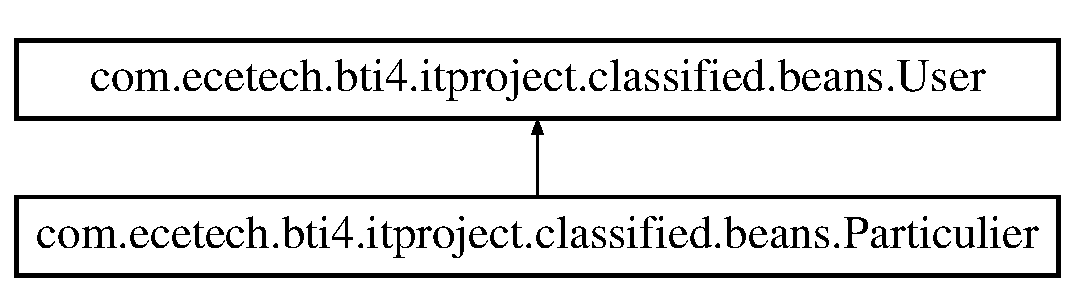
\includegraphics[height=2.000000cm]{classcom_1_1ecetech_1_1bti4_1_1itproject_1_1classified_1_1beans_1_1_particulier}
\end{center}
\end{figure}
\subsection*{Public Member Functions}
\begin{DoxyCompactItemize}
\item 
\hyperlink{classcom_1_1ecetech_1_1bti4_1_1itproject_1_1classified_1_1beans_1_1_particulier_ac4f79bbb0c29d5d8a9711509464d0f68}{Particulier} ()
\item 
\hyperlink{classcom_1_1ecetech_1_1bti4_1_1itproject_1_1classified_1_1beans_1_1_particulier_a8ed9662c72a3880c7d8fcb581d8ec4fb}{Particulier} (String nom\+Part, String prenom\+Part, int num\+Ad\+Part, String rue\+Ad\+Part, int cp\+Ad\+Part, String ville\+Ad\+Part, int tel\+Part)
\item 
String \hyperlink{classcom_1_1ecetech_1_1bti4_1_1itproject_1_1classified_1_1beans_1_1_particulier_a34d82b783f84fe9fe06cd96f4ab0a80b}{get\+Nom\+Part} ()
\item 
void \hyperlink{classcom_1_1ecetech_1_1bti4_1_1itproject_1_1classified_1_1beans_1_1_particulier_a5a5605f2236beb96e21b4eec29e4eef9}{set\+Nom\+Part} (String nom\+Part)
\item 
String \hyperlink{classcom_1_1ecetech_1_1bti4_1_1itproject_1_1classified_1_1beans_1_1_particulier_aba8c676696237418160c042621bea09e}{get\+Prenom\+Part} ()
\item 
void \hyperlink{classcom_1_1ecetech_1_1bti4_1_1itproject_1_1classified_1_1beans_1_1_particulier_a5bf2e8ad1237eff45a6a7d90a69bd099}{set\+Prenom\+Part} (String prenom\+Part)
\item 
int \hyperlink{classcom_1_1ecetech_1_1bti4_1_1itproject_1_1classified_1_1beans_1_1_particulier_ada69990d906d44147eb532df67806ca4}{get\+Num\+Ad\+Part} ()
\item 
void \hyperlink{classcom_1_1ecetech_1_1bti4_1_1itproject_1_1classified_1_1beans_1_1_particulier_a6f4dd50f8bea6a51abdb46b6451cd957}{set\+Num\+Ad\+Part} (int num\+Ad\+Part)
\item 
String \hyperlink{classcom_1_1ecetech_1_1bti4_1_1itproject_1_1classified_1_1beans_1_1_particulier_a2a157dcb18e6d6fec1e6905fb752d29f}{get\+Rue\+Ad\+Part} ()
\item 
void \hyperlink{classcom_1_1ecetech_1_1bti4_1_1itproject_1_1classified_1_1beans_1_1_particulier_a8d9ba90aff12f48a9ab59eb37ea9126e}{set\+Rue\+Ad\+Part} (String rue\+Ad\+Part)
\item 
int \hyperlink{classcom_1_1ecetech_1_1bti4_1_1itproject_1_1classified_1_1beans_1_1_particulier_a0b83dce2a8e0197d5ba536e483331ec9}{get\+Cp\+Ad\+Part} ()
\item 
void \hyperlink{classcom_1_1ecetech_1_1bti4_1_1itproject_1_1classified_1_1beans_1_1_particulier_a3b50f0a2b0f7ddb381cfcd03c73dc9aa}{set\+Cp\+Ad\+Part} (int cp\+Ad\+Part)
\item 
String \hyperlink{classcom_1_1ecetech_1_1bti4_1_1itproject_1_1classified_1_1beans_1_1_particulier_a44996a84395a61f70a55ec96efd54b63}{get\+Ville\+Ad\+Part} ()
\item 
void \hyperlink{classcom_1_1ecetech_1_1bti4_1_1itproject_1_1classified_1_1beans_1_1_particulier_afd20fe3c7eb70e7f26c418e5c7edccd1}{set\+Ville\+Ad\+Part} (String ville\+Ad\+Part)
\item 
int \hyperlink{classcom_1_1ecetech_1_1bti4_1_1itproject_1_1classified_1_1beans_1_1_particulier_a22476481a20d013691e77e7361e876ae}{get\+Tel\+Part} ()
\item 
void \hyperlink{classcom_1_1ecetech_1_1bti4_1_1itproject_1_1classified_1_1beans_1_1_particulier_a2dc8cf8eb4c0b0c867a90b926e63622f}{set\+Tel\+Part} (int tel\+Part)
\item 
String \hyperlink{classcom_1_1ecetech_1_1bti4_1_1itproject_1_1classified_1_1beans_1_1_particulier_ac52a1f1b8e08726f18ff87a20a93ef87}{to\+String} ()
\end{DoxyCompactItemize}


\subsection{Constructor \& Destructor Documentation}
\index{com\+::ecetech\+::bti4\+::itproject\+::classified\+::beans\+::\+Particulier@{com\+::ecetech\+::bti4\+::itproject\+::classified\+::beans\+::\+Particulier}!Particulier@{Particulier}}
\index{Particulier@{Particulier}!com\+::ecetech\+::bti4\+::itproject\+::classified\+::beans\+::\+Particulier@{com\+::ecetech\+::bti4\+::itproject\+::classified\+::beans\+::\+Particulier}}
\subsubsection[{\texorpdfstring{Particulier()}{Particulier()}}]{\setlength{\rightskip}{0pt plus 5cm}com.\+ecetech.\+bti4.\+itproject.\+classified.\+beans.\+Particulier.\+Particulier (
\begin{DoxyParamCaption}
{}
\end{DoxyParamCaption}
)}\hypertarget{classcom_1_1ecetech_1_1bti4_1_1itproject_1_1classified_1_1beans_1_1_particulier_ac4f79bbb0c29d5d8a9711509464d0f68}{}\label{classcom_1_1ecetech_1_1bti4_1_1itproject_1_1classified_1_1beans_1_1_particulier_ac4f79bbb0c29d5d8a9711509464d0f68}
Constructeurs \index{com\+::ecetech\+::bti4\+::itproject\+::classified\+::beans\+::\+Particulier@{com\+::ecetech\+::bti4\+::itproject\+::classified\+::beans\+::\+Particulier}!Particulier@{Particulier}}
\index{Particulier@{Particulier}!com\+::ecetech\+::bti4\+::itproject\+::classified\+::beans\+::\+Particulier@{com\+::ecetech\+::bti4\+::itproject\+::classified\+::beans\+::\+Particulier}}
\subsubsection[{\texorpdfstring{Particulier(\+String nom\+Part, String prenom\+Part, int num\+Ad\+Part, String rue\+Ad\+Part, int cp\+Ad\+Part, String ville\+Ad\+Part, int tel\+Part)}{Particulier(String nomPart, String prenomPart, int numAdPart, String rueAdPart, int cpAdPart, String villeAdPart, int telPart)}}]{\setlength{\rightskip}{0pt plus 5cm}com.\+ecetech.\+bti4.\+itproject.\+classified.\+beans.\+Particulier.\+Particulier (
\begin{DoxyParamCaption}
\item[{String}]{nom\+Part, }
\item[{String}]{prenom\+Part, }
\item[{int}]{num\+Ad\+Part, }
\item[{String}]{rue\+Ad\+Part, }
\item[{int}]{cp\+Ad\+Part, }
\item[{String}]{ville\+Ad\+Part, }
\item[{int}]{tel\+Part}
\end{DoxyParamCaption}
)}\hypertarget{classcom_1_1ecetech_1_1bti4_1_1itproject_1_1classified_1_1beans_1_1_particulier_a8ed9662c72a3880c7d8fcb581d8ec4fb}{}\label{classcom_1_1ecetech_1_1bti4_1_1itproject_1_1classified_1_1beans_1_1_particulier_a8ed9662c72a3880c7d8fcb581d8ec4fb}


\subsection{Member Function Documentation}
\index{com\+::ecetech\+::bti4\+::itproject\+::classified\+::beans\+::\+Particulier@{com\+::ecetech\+::bti4\+::itproject\+::classified\+::beans\+::\+Particulier}!get\+Cp\+Ad\+Part@{get\+Cp\+Ad\+Part}}
\index{get\+Cp\+Ad\+Part@{get\+Cp\+Ad\+Part}!com\+::ecetech\+::bti4\+::itproject\+::classified\+::beans\+::\+Particulier@{com\+::ecetech\+::bti4\+::itproject\+::classified\+::beans\+::\+Particulier}}
\subsubsection[{\texorpdfstring{get\+Cp\+Ad\+Part()}{getCpAdPart()}}]{\setlength{\rightskip}{0pt plus 5cm}int com.\+ecetech.\+bti4.\+itproject.\+classified.\+beans.\+Particulier.\+get\+Cp\+Ad\+Part (
\begin{DoxyParamCaption}
{}
\end{DoxyParamCaption}
)}\hypertarget{classcom_1_1ecetech_1_1bti4_1_1itproject_1_1classified_1_1beans_1_1_particulier_a0b83dce2a8e0197d5ba536e483331ec9}{}\label{classcom_1_1ecetech_1_1bti4_1_1itproject_1_1classified_1_1beans_1_1_particulier_a0b83dce2a8e0197d5ba536e483331ec9}
\index{com\+::ecetech\+::bti4\+::itproject\+::classified\+::beans\+::\+Particulier@{com\+::ecetech\+::bti4\+::itproject\+::classified\+::beans\+::\+Particulier}!get\+Nom\+Part@{get\+Nom\+Part}}
\index{get\+Nom\+Part@{get\+Nom\+Part}!com\+::ecetech\+::bti4\+::itproject\+::classified\+::beans\+::\+Particulier@{com\+::ecetech\+::bti4\+::itproject\+::classified\+::beans\+::\+Particulier}}
\subsubsection[{\texorpdfstring{get\+Nom\+Part()}{getNomPart()}}]{\setlength{\rightskip}{0pt plus 5cm}String com.\+ecetech.\+bti4.\+itproject.\+classified.\+beans.\+Particulier.\+get\+Nom\+Part (
\begin{DoxyParamCaption}
{}
\end{DoxyParamCaption}
)}\hypertarget{classcom_1_1ecetech_1_1bti4_1_1itproject_1_1classified_1_1beans_1_1_particulier_a34d82b783f84fe9fe06cd96f4ab0a80b}{}\label{classcom_1_1ecetech_1_1bti4_1_1itproject_1_1classified_1_1beans_1_1_particulier_a34d82b783f84fe9fe06cd96f4ab0a80b}
Getters \& Setters \index{com\+::ecetech\+::bti4\+::itproject\+::classified\+::beans\+::\+Particulier@{com\+::ecetech\+::bti4\+::itproject\+::classified\+::beans\+::\+Particulier}!get\+Num\+Ad\+Part@{get\+Num\+Ad\+Part}}
\index{get\+Num\+Ad\+Part@{get\+Num\+Ad\+Part}!com\+::ecetech\+::bti4\+::itproject\+::classified\+::beans\+::\+Particulier@{com\+::ecetech\+::bti4\+::itproject\+::classified\+::beans\+::\+Particulier}}
\subsubsection[{\texorpdfstring{get\+Num\+Ad\+Part()}{getNumAdPart()}}]{\setlength{\rightskip}{0pt plus 5cm}int com.\+ecetech.\+bti4.\+itproject.\+classified.\+beans.\+Particulier.\+get\+Num\+Ad\+Part (
\begin{DoxyParamCaption}
{}
\end{DoxyParamCaption}
)}\hypertarget{classcom_1_1ecetech_1_1bti4_1_1itproject_1_1classified_1_1beans_1_1_particulier_ada69990d906d44147eb532df67806ca4}{}\label{classcom_1_1ecetech_1_1bti4_1_1itproject_1_1classified_1_1beans_1_1_particulier_ada69990d906d44147eb532df67806ca4}
\index{com\+::ecetech\+::bti4\+::itproject\+::classified\+::beans\+::\+Particulier@{com\+::ecetech\+::bti4\+::itproject\+::classified\+::beans\+::\+Particulier}!get\+Prenom\+Part@{get\+Prenom\+Part}}
\index{get\+Prenom\+Part@{get\+Prenom\+Part}!com\+::ecetech\+::bti4\+::itproject\+::classified\+::beans\+::\+Particulier@{com\+::ecetech\+::bti4\+::itproject\+::classified\+::beans\+::\+Particulier}}
\subsubsection[{\texorpdfstring{get\+Prenom\+Part()}{getPrenomPart()}}]{\setlength{\rightskip}{0pt plus 5cm}String com.\+ecetech.\+bti4.\+itproject.\+classified.\+beans.\+Particulier.\+get\+Prenom\+Part (
\begin{DoxyParamCaption}
{}
\end{DoxyParamCaption}
)}\hypertarget{classcom_1_1ecetech_1_1bti4_1_1itproject_1_1classified_1_1beans_1_1_particulier_aba8c676696237418160c042621bea09e}{}\label{classcom_1_1ecetech_1_1bti4_1_1itproject_1_1classified_1_1beans_1_1_particulier_aba8c676696237418160c042621bea09e}
\index{com\+::ecetech\+::bti4\+::itproject\+::classified\+::beans\+::\+Particulier@{com\+::ecetech\+::bti4\+::itproject\+::classified\+::beans\+::\+Particulier}!get\+Rue\+Ad\+Part@{get\+Rue\+Ad\+Part}}
\index{get\+Rue\+Ad\+Part@{get\+Rue\+Ad\+Part}!com\+::ecetech\+::bti4\+::itproject\+::classified\+::beans\+::\+Particulier@{com\+::ecetech\+::bti4\+::itproject\+::classified\+::beans\+::\+Particulier}}
\subsubsection[{\texorpdfstring{get\+Rue\+Ad\+Part()}{getRueAdPart()}}]{\setlength{\rightskip}{0pt plus 5cm}String com.\+ecetech.\+bti4.\+itproject.\+classified.\+beans.\+Particulier.\+get\+Rue\+Ad\+Part (
\begin{DoxyParamCaption}
{}
\end{DoxyParamCaption}
)}\hypertarget{classcom_1_1ecetech_1_1bti4_1_1itproject_1_1classified_1_1beans_1_1_particulier_a2a157dcb18e6d6fec1e6905fb752d29f}{}\label{classcom_1_1ecetech_1_1bti4_1_1itproject_1_1classified_1_1beans_1_1_particulier_a2a157dcb18e6d6fec1e6905fb752d29f}
\index{com\+::ecetech\+::bti4\+::itproject\+::classified\+::beans\+::\+Particulier@{com\+::ecetech\+::bti4\+::itproject\+::classified\+::beans\+::\+Particulier}!get\+Tel\+Part@{get\+Tel\+Part}}
\index{get\+Tel\+Part@{get\+Tel\+Part}!com\+::ecetech\+::bti4\+::itproject\+::classified\+::beans\+::\+Particulier@{com\+::ecetech\+::bti4\+::itproject\+::classified\+::beans\+::\+Particulier}}
\subsubsection[{\texorpdfstring{get\+Tel\+Part()}{getTelPart()}}]{\setlength{\rightskip}{0pt plus 5cm}int com.\+ecetech.\+bti4.\+itproject.\+classified.\+beans.\+Particulier.\+get\+Tel\+Part (
\begin{DoxyParamCaption}
{}
\end{DoxyParamCaption}
)}\hypertarget{classcom_1_1ecetech_1_1bti4_1_1itproject_1_1classified_1_1beans_1_1_particulier_a22476481a20d013691e77e7361e876ae}{}\label{classcom_1_1ecetech_1_1bti4_1_1itproject_1_1classified_1_1beans_1_1_particulier_a22476481a20d013691e77e7361e876ae}
\index{com\+::ecetech\+::bti4\+::itproject\+::classified\+::beans\+::\+Particulier@{com\+::ecetech\+::bti4\+::itproject\+::classified\+::beans\+::\+Particulier}!get\+Ville\+Ad\+Part@{get\+Ville\+Ad\+Part}}
\index{get\+Ville\+Ad\+Part@{get\+Ville\+Ad\+Part}!com\+::ecetech\+::bti4\+::itproject\+::classified\+::beans\+::\+Particulier@{com\+::ecetech\+::bti4\+::itproject\+::classified\+::beans\+::\+Particulier}}
\subsubsection[{\texorpdfstring{get\+Ville\+Ad\+Part()}{getVilleAdPart()}}]{\setlength{\rightskip}{0pt plus 5cm}String com.\+ecetech.\+bti4.\+itproject.\+classified.\+beans.\+Particulier.\+get\+Ville\+Ad\+Part (
\begin{DoxyParamCaption}
{}
\end{DoxyParamCaption}
)}\hypertarget{classcom_1_1ecetech_1_1bti4_1_1itproject_1_1classified_1_1beans_1_1_particulier_a44996a84395a61f70a55ec96efd54b63}{}\label{classcom_1_1ecetech_1_1bti4_1_1itproject_1_1classified_1_1beans_1_1_particulier_a44996a84395a61f70a55ec96efd54b63}
\index{com\+::ecetech\+::bti4\+::itproject\+::classified\+::beans\+::\+Particulier@{com\+::ecetech\+::bti4\+::itproject\+::classified\+::beans\+::\+Particulier}!set\+Cp\+Ad\+Part@{set\+Cp\+Ad\+Part}}
\index{set\+Cp\+Ad\+Part@{set\+Cp\+Ad\+Part}!com\+::ecetech\+::bti4\+::itproject\+::classified\+::beans\+::\+Particulier@{com\+::ecetech\+::bti4\+::itproject\+::classified\+::beans\+::\+Particulier}}
\subsubsection[{\texorpdfstring{set\+Cp\+Ad\+Part(int cp\+Ad\+Part)}{setCpAdPart(int cpAdPart)}}]{\setlength{\rightskip}{0pt plus 5cm}void com.\+ecetech.\+bti4.\+itproject.\+classified.\+beans.\+Particulier.\+set\+Cp\+Ad\+Part (
\begin{DoxyParamCaption}
\item[{int}]{cp\+Ad\+Part}
\end{DoxyParamCaption}
)}\hypertarget{classcom_1_1ecetech_1_1bti4_1_1itproject_1_1classified_1_1beans_1_1_particulier_a3b50f0a2b0f7ddb381cfcd03c73dc9aa}{}\label{classcom_1_1ecetech_1_1bti4_1_1itproject_1_1classified_1_1beans_1_1_particulier_a3b50f0a2b0f7ddb381cfcd03c73dc9aa}
\index{com\+::ecetech\+::bti4\+::itproject\+::classified\+::beans\+::\+Particulier@{com\+::ecetech\+::bti4\+::itproject\+::classified\+::beans\+::\+Particulier}!set\+Nom\+Part@{set\+Nom\+Part}}
\index{set\+Nom\+Part@{set\+Nom\+Part}!com\+::ecetech\+::bti4\+::itproject\+::classified\+::beans\+::\+Particulier@{com\+::ecetech\+::bti4\+::itproject\+::classified\+::beans\+::\+Particulier}}
\subsubsection[{\texorpdfstring{set\+Nom\+Part(\+String nom\+Part)}{setNomPart(String nomPart)}}]{\setlength{\rightskip}{0pt plus 5cm}void com.\+ecetech.\+bti4.\+itproject.\+classified.\+beans.\+Particulier.\+set\+Nom\+Part (
\begin{DoxyParamCaption}
\item[{String}]{nom\+Part}
\end{DoxyParamCaption}
)}\hypertarget{classcom_1_1ecetech_1_1bti4_1_1itproject_1_1classified_1_1beans_1_1_particulier_a5a5605f2236beb96e21b4eec29e4eef9}{}\label{classcom_1_1ecetech_1_1bti4_1_1itproject_1_1classified_1_1beans_1_1_particulier_a5a5605f2236beb96e21b4eec29e4eef9}
\index{com\+::ecetech\+::bti4\+::itproject\+::classified\+::beans\+::\+Particulier@{com\+::ecetech\+::bti4\+::itproject\+::classified\+::beans\+::\+Particulier}!set\+Num\+Ad\+Part@{set\+Num\+Ad\+Part}}
\index{set\+Num\+Ad\+Part@{set\+Num\+Ad\+Part}!com\+::ecetech\+::bti4\+::itproject\+::classified\+::beans\+::\+Particulier@{com\+::ecetech\+::bti4\+::itproject\+::classified\+::beans\+::\+Particulier}}
\subsubsection[{\texorpdfstring{set\+Num\+Ad\+Part(int num\+Ad\+Part)}{setNumAdPart(int numAdPart)}}]{\setlength{\rightskip}{0pt plus 5cm}void com.\+ecetech.\+bti4.\+itproject.\+classified.\+beans.\+Particulier.\+set\+Num\+Ad\+Part (
\begin{DoxyParamCaption}
\item[{int}]{num\+Ad\+Part}
\end{DoxyParamCaption}
)}\hypertarget{classcom_1_1ecetech_1_1bti4_1_1itproject_1_1classified_1_1beans_1_1_particulier_a6f4dd50f8bea6a51abdb46b6451cd957}{}\label{classcom_1_1ecetech_1_1bti4_1_1itproject_1_1classified_1_1beans_1_1_particulier_a6f4dd50f8bea6a51abdb46b6451cd957}
\index{com\+::ecetech\+::bti4\+::itproject\+::classified\+::beans\+::\+Particulier@{com\+::ecetech\+::bti4\+::itproject\+::classified\+::beans\+::\+Particulier}!set\+Prenom\+Part@{set\+Prenom\+Part}}
\index{set\+Prenom\+Part@{set\+Prenom\+Part}!com\+::ecetech\+::bti4\+::itproject\+::classified\+::beans\+::\+Particulier@{com\+::ecetech\+::bti4\+::itproject\+::classified\+::beans\+::\+Particulier}}
\subsubsection[{\texorpdfstring{set\+Prenom\+Part(\+String prenom\+Part)}{setPrenomPart(String prenomPart)}}]{\setlength{\rightskip}{0pt plus 5cm}void com.\+ecetech.\+bti4.\+itproject.\+classified.\+beans.\+Particulier.\+set\+Prenom\+Part (
\begin{DoxyParamCaption}
\item[{String}]{prenom\+Part}
\end{DoxyParamCaption}
)}\hypertarget{classcom_1_1ecetech_1_1bti4_1_1itproject_1_1classified_1_1beans_1_1_particulier_a5bf2e8ad1237eff45a6a7d90a69bd099}{}\label{classcom_1_1ecetech_1_1bti4_1_1itproject_1_1classified_1_1beans_1_1_particulier_a5bf2e8ad1237eff45a6a7d90a69bd099}
\index{com\+::ecetech\+::bti4\+::itproject\+::classified\+::beans\+::\+Particulier@{com\+::ecetech\+::bti4\+::itproject\+::classified\+::beans\+::\+Particulier}!set\+Rue\+Ad\+Part@{set\+Rue\+Ad\+Part}}
\index{set\+Rue\+Ad\+Part@{set\+Rue\+Ad\+Part}!com\+::ecetech\+::bti4\+::itproject\+::classified\+::beans\+::\+Particulier@{com\+::ecetech\+::bti4\+::itproject\+::classified\+::beans\+::\+Particulier}}
\subsubsection[{\texorpdfstring{set\+Rue\+Ad\+Part(\+String rue\+Ad\+Part)}{setRueAdPart(String rueAdPart)}}]{\setlength{\rightskip}{0pt plus 5cm}void com.\+ecetech.\+bti4.\+itproject.\+classified.\+beans.\+Particulier.\+set\+Rue\+Ad\+Part (
\begin{DoxyParamCaption}
\item[{String}]{rue\+Ad\+Part}
\end{DoxyParamCaption}
)}\hypertarget{classcom_1_1ecetech_1_1bti4_1_1itproject_1_1classified_1_1beans_1_1_particulier_a8d9ba90aff12f48a9ab59eb37ea9126e}{}\label{classcom_1_1ecetech_1_1bti4_1_1itproject_1_1classified_1_1beans_1_1_particulier_a8d9ba90aff12f48a9ab59eb37ea9126e}
\index{com\+::ecetech\+::bti4\+::itproject\+::classified\+::beans\+::\+Particulier@{com\+::ecetech\+::bti4\+::itproject\+::classified\+::beans\+::\+Particulier}!set\+Tel\+Part@{set\+Tel\+Part}}
\index{set\+Tel\+Part@{set\+Tel\+Part}!com\+::ecetech\+::bti4\+::itproject\+::classified\+::beans\+::\+Particulier@{com\+::ecetech\+::bti4\+::itproject\+::classified\+::beans\+::\+Particulier}}
\subsubsection[{\texorpdfstring{set\+Tel\+Part(int tel\+Part)}{setTelPart(int telPart)}}]{\setlength{\rightskip}{0pt plus 5cm}void com.\+ecetech.\+bti4.\+itproject.\+classified.\+beans.\+Particulier.\+set\+Tel\+Part (
\begin{DoxyParamCaption}
\item[{int}]{tel\+Part}
\end{DoxyParamCaption}
)}\hypertarget{classcom_1_1ecetech_1_1bti4_1_1itproject_1_1classified_1_1beans_1_1_particulier_a2dc8cf8eb4c0b0c867a90b926e63622f}{}\label{classcom_1_1ecetech_1_1bti4_1_1itproject_1_1classified_1_1beans_1_1_particulier_a2dc8cf8eb4c0b0c867a90b926e63622f}
\index{com\+::ecetech\+::bti4\+::itproject\+::classified\+::beans\+::\+Particulier@{com\+::ecetech\+::bti4\+::itproject\+::classified\+::beans\+::\+Particulier}!set\+Ville\+Ad\+Part@{set\+Ville\+Ad\+Part}}
\index{set\+Ville\+Ad\+Part@{set\+Ville\+Ad\+Part}!com\+::ecetech\+::bti4\+::itproject\+::classified\+::beans\+::\+Particulier@{com\+::ecetech\+::bti4\+::itproject\+::classified\+::beans\+::\+Particulier}}
\subsubsection[{\texorpdfstring{set\+Ville\+Ad\+Part(\+String ville\+Ad\+Part)}{setVilleAdPart(String villeAdPart)}}]{\setlength{\rightskip}{0pt plus 5cm}void com.\+ecetech.\+bti4.\+itproject.\+classified.\+beans.\+Particulier.\+set\+Ville\+Ad\+Part (
\begin{DoxyParamCaption}
\item[{String}]{ville\+Ad\+Part}
\end{DoxyParamCaption}
)}\hypertarget{classcom_1_1ecetech_1_1bti4_1_1itproject_1_1classified_1_1beans_1_1_particulier_afd20fe3c7eb70e7f26c418e5c7edccd1}{}\label{classcom_1_1ecetech_1_1bti4_1_1itproject_1_1classified_1_1beans_1_1_particulier_afd20fe3c7eb70e7f26c418e5c7edccd1}
\index{com\+::ecetech\+::bti4\+::itproject\+::classified\+::beans\+::\+Particulier@{com\+::ecetech\+::bti4\+::itproject\+::classified\+::beans\+::\+Particulier}!to\+String@{to\+String}}
\index{to\+String@{to\+String}!com\+::ecetech\+::bti4\+::itproject\+::classified\+::beans\+::\+Particulier@{com\+::ecetech\+::bti4\+::itproject\+::classified\+::beans\+::\+Particulier}}
\subsubsection[{\texorpdfstring{to\+String()}{toString()}}]{\setlength{\rightskip}{0pt plus 5cm}String com.\+ecetech.\+bti4.\+itproject.\+classified.\+beans.\+Particulier.\+to\+String (
\begin{DoxyParamCaption}
{}
\end{DoxyParamCaption}
)}\hypertarget{classcom_1_1ecetech_1_1bti4_1_1itproject_1_1classified_1_1beans_1_1_particulier_ac52a1f1b8e08726f18ff87a20a93ef87}{}\label{classcom_1_1ecetech_1_1bti4_1_1itproject_1_1classified_1_1beans_1_1_particulier_ac52a1f1b8e08726f18ff87a20a93ef87}


The documentation for this class was generated from the following file\+:\begin{DoxyCompactItemize}
\item 
Classified-\/\+Model/src/com/ecetech/bti4/itproject/classified/beans/\hyperlink{_particulier_8java}{Particulier.\+java}\end{DoxyCompactItemize}

\hypertarget{classcom_1_1ecetech_1_1bti4_1_1itproject_1_1classified_1_1dao_1_1_particulier_d_a_o}{}\section{com.\+ecetech.\+bti4.\+itproject.\+classified.\+dao.\+Particulier\+D\+AO Class Reference}
\label{classcom_1_1ecetech_1_1bti4_1_1itproject_1_1classified_1_1dao_1_1_particulier_d_a_o}\index{com.\+ecetech.\+bti4.\+itproject.\+classified.\+dao.\+Particulier\+D\+AO@{com.\+ecetech.\+bti4.\+itproject.\+classified.\+dao.\+Particulier\+D\+AO}}
\subsection*{Static Public Member Functions}
\begin{DoxyCompactItemize}
\item 
static \hyperlink{classcom_1_1ecetech_1_1bti4_1_1itproject_1_1classified_1_1beans_1_1_particulier}{Particulier} \hyperlink{classcom_1_1ecetech_1_1bti4_1_1itproject_1_1classified_1_1dao_1_1_particulier_d_a_o_ac0301dfbee89d579eda92e8bce0b3adc}{get\+Part\+User} (String id\+User)  throws S\+Q\+L\+Exception 
\item 
static void \hyperlink{classcom_1_1ecetech_1_1bti4_1_1itproject_1_1classified_1_1dao_1_1_particulier_d_a_o_a6ae4d4a053c195c408910fb795e1d075}{add\+Part\+User} (String Mail\+User, String Mdp\+User, String Permission\+User, String Nom\+Part, String Prenom\+Part, int Num\+Ad\+Part, String Rue\+Ad\+Part, int Cp\+Ad\+Part, String Ville\+Ad\+Part, int Tel\+Part)  throws S\+Q\+L\+Exception 
\item 
static void \hyperlink{classcom_1_1ecetech_1_1bti4_1_1itproject_1_1classified_1_1dao_1_1_particulier_d_a_o_a98be8767197256f613505cc57f63e17e}{update\+Nom\+Part} (String id\+User, String nom\+Part)  throws S\+Q\+L\+Exception 
\item 
static void \hyperlink{classcom_1_1ecetech_1_1bti4_1_1itproject_1_1classified_1_1dao_1_1_particulier_d_a_o_a254445b06718d384521fdb9579ceeffe}{update\+Prenom\+Part} (String id\+User, String prenom\+Part)  throws S\+Q\+L\+Exception 
\item 
static void \hyperlink{classcom_1_1ecetech_1_1bti4_1_1itproject_1_1classified_1_1dao_1_1_particulier_d_a_o_acedb245e7cae04b12565c22e959f27cf}{update\+Num\+Ad\+Part} (String id\+User, int num\+Ad\+Part)  throws S\+Q\+L\+Exception 
\item 
static void \hyperlink{classcom_1_1ecetech_1_1bti4_1_1itproject_1_1classified_1_1dao_1_1_particulier_d_a_o_a7e2a2890658c990d31f9df3d75ca0b4e}{update\+Rue\+Ad\+Part} (String id\+User, String rue\+Ad\+Part)  throws S\+Q\+L\+Exception 
\item 
static void \hyperlink{classcom_1_1ecetech_1_1bti4_1_1itproject_1_1classified_1_1dao_1_1_particulier_d_a_o_ada1b25c056da3b0e4b1fe9b9f32bbe47}{update\+Cp\+Ad\+Part} (String id\+User, int cp\+Ad\+Part)  throws S\+Q\+L\+Exception 
\item 
static void \hyperlink{classcom_1_1ecetech_1_1bti4_1_1itproject_1_1classified_1_1dao_1_1_particulier_d_a_o_aa902ab4baffe2f3d01ab2d652d084e57}{update\+Ville\+Ad\+Part} (String id\+User, String Ville\+Ad\+Part)  throws S\+Q\+L\+Exception 
\item 
static void \hyperlink{classcom_1_1ecetech_1_1bti4_1_1itproject_1_1classified_1_1dao_1_1_particulier_d_a_o_a1bf005b9911ce09d8daa26abf9fdf04e}{update\+Tel\+Part} (String id\+User, int Tel\+Part)  throws S\+Q\+L\+Exception 
\end{DoxyCompactItemize}


\subsection{Detailed Description}
Represente un particulier \begin{DoxyAuthor}{Author}
Maeva, Adrien, Moaz 
\end{DoxyAuthor}


\subsection{Member Function Documentation}
\index{com\+::ecetech\+::bti4\+::itproject\+::classified\+::dao\+::\+Particulier\+D\+AO@{com\+::ecetech\+::bti4\+::itproject\+::classified\+::dao\+::\+Particulier\+D\+AO}!add\+Part\+User@{add\+Part\+User}}
\index{add\+Part\+User@{add\+Part\+User}!com\+::ecetech\+::bti4\+::itproject\+::classified\+::dao\+::\+Particulier\+D\+AO@{com\+::ecetech\+::bti4\+::itproject\+::classified\+::dao\+::\+Particulier\+D\+AO}}
\subsubsection[{\texorpdfstring{add\+Part\+User(\+String Mail\+User, String Mdp\+User, String Permission\+User, String Nom\+Part, String Prenom\+Part, int Num\+Ad\+Part, String Rue\+Ad\+Part, int Cp\+Ad\+Part, String Ville\+Ad\+Part, int Tel\+Part)}{addPartUser(String MailUser, String MdpUser, String PermissionUser, String NomPart, String PrenomPart, int NumAdPart, String RueAdPart, int CpAdPart, String VilleAdPart, int TelPart)}}]{\setlength{\rightskip}{0pt plus 5cm}static void com.\+ecetech.\+bti4.\+itproject.\+classified.\+dao.\+Particulier\+D\+A\+O.\+add\+Part\+User (
\begin{DoxyParamCaption}
\item[{String}]{Mail\+User, }
\item[{String}]{Mdp\+User, }
\item[{String}]{Permission\+User, }
\item[{String}]{Nom\+Part, }
\item[{String}]{Prenom\+Part, }
\item[{int}]{Num\+Ad\+Part, }
\item[{String}]{Rue\+Ad\+Part, }
\item[{int}]{Cp\+Ad\+Part, }
\item[{String}]{Ville\+Ad\+Part, }
\item[{int}]{Tel\+Part}
\end{DoxyParamCaption}
) throws S\+Q\+L\+Exception\hspace{0.3cm}{\ttfamily [static]}}\hypertarget{classcom_1_1ecetech_1_1bti4_1_1itproject_1_1classified_1_1dao_1_1_particulier_d_a_o_a6ae4d4a053c195c408910fb795e1d075}{}\label{classcom_1_1ecetech_1_1bti4_1_1itproject_1_1classified_1_1dao_1_1_particulier_d_a_o_a6ae4d4a053c195c408910fb795e1d075}
public fonction \hyperlink{classcom_1_1ecetech_1_1bti4_1_1itproject_1_1classified_1_1dao_1_1_particulier_d_a_o_a6ae4d4a053c195c408910fb795e1d075}{add\+Part\+User()}  Modifie un particulier

Ne renvoie rien \index{com\+::ecetech\+::bti4\+::itproject\+::classified\+::dao\+::\+Particulier\+D\+AO@{com\+::ecetech\+::bti4\+::itproject\+::classified\+::dao\+::\+Particulier\+D\+AO}!get\+Part\+User@{get\+Part\+User}}
\index{get\+Part\+User@{get\+Part\+User}!com\+::ecetech\+::bti4\+::itproject\+::classified\+::dao\+::\+Particulier\+D\+AO@{com\+::ecetech\+::bti4\+::itproject\+::classified\+::dao\+::\+Particulier\+D\+AO}}
\subsubsection[{\texorpdfstring{get\+Part\+User(\+String id\+User)}{getPartUser(String idUser)}}]{\setlength{\rightskip}{0pt plus 5cm}static {\bf Particulier} com.\+ecetech.\+bti4.\+itproject.\+classified.\+dao.\+Particulier\+D\+A\+O.\+get\+Part\+User (
\begin{DoxyParamCaption}
\item[{String}]{id\+User}
\end{DoxyParamCaption}
) throws S\+Q\+L\+Exception\hspace{0.3cm}{\ttfamily [static]}}\hypertarget{classcom_1_1ecetech_1_1bti4_1_1itproject_1_1classified_1_1dao_1_1_particulier_d_a_o_ac0301dfbee89d579eda92e8bce0b3adc}{}\label{classcom_1_1ecetech_1_1bti4_1_1itproject_1_1classified_1_1dao_1_1_particulier_d_a_o_ac0301dfbee89d579eda92e8bce0b3adc}
public fonction get\+Partt\+User()  Affiche un particulier

Renvoie une Arraylist contenant un particulier de la base de donnee \index{com\+::ecetech\+::bti4\+::itproject\+::classified\+::dao\+::\+Particulier\+D\+AO@{com\+::ecetech\+::bti4\+::itproject\+::classified\+::dao\+::\+Particulier\+D\+AO}!update\+Cp\+Ad\+Part@{update\+Cp\+Ad\+Part}}
\index{update\+Cp\+Ad\+Part@{update\+Cp\+Ad\+Part}!com\+::ecetech\+::bti4\+::itproject\+::classified\+::dao\+::\+Particulier\+D\+AO@{com\+::ecetech\+::bti4\+::itproject\+::classified\+::dao\+::\+Particulier\+D\+AO}}
\subsubsection[{\texorpdfstring{update\+Cp\+Ad\+Part(\+String id\+User, int cp\+Ad\+Part)}{updateCpAdPart(String idUser, int cpAdPart)}}]{\setlength{\rightskip}{0pt plus 5cm}static void com.\+ecetech.\+bti4.\+itproject.\+classified.\+dao.\+Particulier\+D\+A\+O.\+update\+Cp\+Ad\+Part (
\begin{DoxyParamCaption}
\item[{String}]{id\+User, }
\item[{int}]{cp\+Ad\+Part}
\end{DoxyParamCaption}
) throws S\+Q\+L\+Exception\hspace{0.3cm}{\ttfamily [static]}}\hypertarget{classcom_1_1ecetech_1_1bti4_1_1itproject_1_1classified_1_1dao_1_1_particulier_d_a_o_ada1b25c056da3b0e4b1fe9b9f32bbe47}{}\label{classcom_1_1ecetech_1_1bti4_1_1itproject_1_1classified_1_1dao_1_1_particulier_d_a_o_ada1b25c056da3b0e4b1fe9b9f32bbe47}
public fonction \hyperlink{classcom_1_1ecetech_1_1bti4_1_1itproject_1_1classified_1_1dao_1_1_particulier_d_a_o_ada1b25c056da3b0e4b1fe9b9f32bbe47}{update\+Cp\+Ad\+Part()}  Modifie le code postale d\textquotesingle{}un particulier

Ne renvoie rien \index{com\+::ecetech\+::bti4\+::itproject\+::classified\+::dao\+::\+Particulier\+D\+AO@{com\+::ecetech\+::bti4\+::itproject\+::classified\+::dao\+::\+Particulier\+D\+AO}!update\+Nom\+Part@{update\+Nom\+Part}}
\index{update\+Nom\+Part@{update\+Nom\+Part}!com\+::ecetech\+::bti4\+::itproject\+::classified\+::dao\+::\+Particulier\+D\+AO@{com\+::ecetech\+::bti4\+::itproject\+::classified\+::dao\+::\+Particulier\+D\+AO}}
\subsubsection[{\texorpdfstring{update\+Nom\+Part(\+String id\+User, String nom\+Part)}{updateNomPart(String idUser, String nomPart)}}]{\setlength{\rightskip}{0pt plus 5cm}static void com.\+ecetech.\+bti4.\+itproject.\+classified.\+dao.\+Particulier\+D\+A\+O.\+update\+Nom\+Part (
\begin{DoxyParamCaption}
\item[{String}]{id\+User, }
\item[{String}]{nom\+Part}
\end{DoxyParamCaption}
) throws S\+Q\+L\+Exception\hspace{0.3cm}{\ttfamily [static]}}\hypertarget{classcom_1_1ecetech_1_1bti4_1_1itproject_1_1classified_1_1dao_1_1_particulier_d_a_o_a98be8767197256f613505cc57f63e17e}{}\label{classcom_1_1ecetech_1_1bti4_1_1itproject_1_1classified_1_1dao_1_1_particulier_d_a_o_a98be8767197256f613505cc57f63e17e}
public fonction \hyperlink{classcom_1_1ecetech_1_1bti4_1_1itproject_1_1classified_1_1dao_1_1_particulier_d_a_o_a98be8767197256f613505cc57f63e17e}{update\+Nom\+Part()}  Modifie le nom d\textquotesingle{}un particulier

Ne renvoie rien \index{com\+::ecetech\+::bti4\+::itproject\+::classified\+::dao\+::\+Particulier\+D\+AO@{com\+::ecetech\+::bti4\+::itproject\+::classified\+::dao\+::\+Particulier\+D\+AO}!update\+Num\+Ad\+Part@{update\+Num\+Ad\+Part}}
\index{update\+Num\+Ad\+Part@{update\+Num\+Ad\+Part}!com\+::ecetech\+::bti4\+::itproject\+::classified\+::dao\+::\+Particulier\+D\+AO@{com\+::ecetech\+::bti4\+::itproject\+::classified\+::dao\+::\+Particulier\+D\+AO}}
\subsubsection[{\texorpdfstring{update\+Num\+Ad\+Part(\+String id\+User, int num\+Ad\+Part)}{updateNumAdPart(String idUser, int numAdPart)}}]{\setlength{\rightskip}{0pt plus 5cm}static void com.\+ecetech.\+bti4.\+itproject.\+classified.\+dao.\+Particulier\+D\+A\+O.\+update\+Num\+Ad\+Part (
\begin{DoxyParamCaption}
\item[{String}]{id\+User, }
\item[{int}]{num\+Ad\+Part}
\end{DoxyParamCaption}
) throws S\+Q\+L\+Exception\hspace{0.3cm}{\ttfamily [static]}}\hypertarget{classcom_1_1ecetech_1_1bti4_1_1itproject_1_1classified_1_1dao_1_1_particulier_d_a_o_acedb245e7cae04b12565c22e959f27cf}{}\label{classcom_1_1ecetech_1_1bti4_1_1itproject_1_1classified_1_1dao_1_1_particulier_d_a_o_acedb245e7cae04b12565c22e959f27cf}
public fonction \hyperlink{classcom_1_1ecetech_1_1bti4_1_1itproject_1_1classified_1_1dao_1_1_particulier_d_a_o_acedb245e7cae04b12565c22e959f27cf}{update\+Num\+Ad\+Part()}  Modifie le numero de telephone d\textquotesingle{}un particulier

Ne renvoie rien \index{com\+::ecetech\+::bti4\+::itproject\+::classified\+::dao\+::\+Particulier\+D\+AO@{com\+::ecetech\+::bti4\+::itproject\+::classified\+::dao\+::\+Particulier\+D\+AO}!update\+Prenom\+Part@{update\+Prenom\+Part}}
\index{update\+Prenom\+Part@{update\+Prenom\+Part}!com\+::ecetech\+::bti4\+::itproject\+::classified\+::dao\+::\+Particulier\+D\+AO@{com\+::ecetech\+::bti4\+::itproject\+::classified\+::dao\+::\+Particulier\+D\+AO}}
\subsubsection[{\texorpdfstring{update\+Prenom\+Part(\+String id\+User, String prenom\+Part)}{updatePrenomPart(String idUser, String prenomPart)}}]{\setlength{\rightskip}{0pt plus 5cm}static void com.\+ecetech.\+bti4.\+itproject.\+classified.\+dao.\+Particulier\+D\+A\+O.\+update\+Prenom\+Part (
\begin{DoxyParamCaption}
\item[{String}]{id\+User, }
\item[{String}]{prenom\+Part}
\end{DoxyParamCaption}
) throws S\+Q\+L\+Exception\hspace{0.3cm}{\ttfamily [static]}}\hypertarget{classcom_1_1ecetech_1_1bti4_1_1itproject_1_1classified_1_1dao_1_1_particulier_d_a_o_a254445b06718d384521fdb9579ceeffe}{}\label{classcom_1_1ecetech_1_1bti4_1_1itproject_1_1classified_1_1dao_1_1_particulier_d_a_o_a254445b06718d384521fdb9579ceeffe}
public fonction \hyperlink{classcom_1_1ecetech_1_1bti4_1_1itproject_1_1classified_1_1dao_1_1_particulier_d_a_o_a254445b06718d384521fdb9579ceeffe}{update\+Prenom\+Part()}  Modifie le prenom d\textquotesingle{}un particulier

Ne renvoie rien \index{com\+::ecetech\+::bti4\+::itproject\+::classified\+::dao\+::\+Particulier\+D\+AO@{com\+::ecetech\+::bti4\+::itproject\+::classified\+::dao\+::\+Particulier\+D\+AO}!update\+Rue\+Ad\+Part@{update\+Rue\+Ad\+Part}}
\index{update\+Rue\+Ad\+Part@{update\+Rue\+Ad\+Part}!com\+::ecetech\+::bti4\+::itproject\+::classified\+::dao\+::\+Particulier\+D\+AO@{com\+::ecetech\+::bti4\+::itproject\+::classified\+::dao\+::\+Particulier\+D\+AO}}
\subsubsection[{\texorpdfstring{update\+Rue\+Ad\+Part(\+String id\+User, String rue\+Ad\+Part)}{updateRueAdPart(String idUser, String rueAdPart)}}]{\setlength{\rightskip}{0pt plus 5cm}static void com.\+ecetech.\+bti4.\+itproject.\+classified.\+dao.\+Particulier\+D\+A\+O.\+update\+Rue\+Ad\+Part (
\begin{DoxyParamCaption}
\item[{String}]{id\+User, }
\item[{String}]{rue\+Ad\+Part}
\end{DoxyParamCaption}
) throws S\+Q\+L\+Exception\hspace{0.3cm}{\ttfamily [static]}}\hypertarget{classcom_1_1ecetech_1_1bti4_1_1itproject_1_1classified_1_1dao_1_1_particulier_d_a_o_a7e2a2890658c990d31f9df3d75ca0b4e}{}\label{classcom_1_1ecetech_1_1bti4_1_1itproject_1_1classified_1_1dao_1_1_particulier_d_a_o_a7e2a2890658c990d31f9df3d75ca0b4e}
public fonction \hyperlink{classcom_1_1ecetech_1_1bti4_1_1itproject_1_1classified_1_1dao_1_1_particulier_d_a_o_a7e2a2890658c990d31f9df3d75ca0b4e}{update\+Rue\+Ad\+Part()}  Modifie la rue de l\textquotesingle{}adresse d\textquotesingle{}un particulier

Ne renvoie rien \index{com\+::ecetech\+::bti4\+::itproject\+::classified\+::dao\+::\+Particulier\+D\+AO@{com\+::ecetech\+::bti4\+::itproject\+::classified\+::dao\+::\+Particulier\+D\+AO}!update\+Tel\+Part@{update\+Tel\+Part}}
\index{update\+Tel\+Part@{update\+Tel\+Part}!com\+::ecetech\+::bti4\+::itproject\+::classified\+::dao\+::\+Particulier\+D\+AO@{com\+::ecetech\+::bti4\+::itproject\+::classified\+::dao\+::\+Particulier\+D\+AO}}
\subsubsection[{\texorpdfstring{update\+Tel\+Part(\+String id\+User, int Tel\+Part)}{updateTelPart(String idUser, int TelPart)}}]{\setlength{\rightskip}{0pt plus 5cm}static void com.\+ecetech.\+bti4.\+itproject.\+classified.\+dao.\+Particulier\+D\+A\+O.\+update\+Tel\+Part (
\begin{DoxyParamCaption}
\item[{String}]{id\+User, }
\item[{int}]{Tel\+Part}
\end{DoxyParamCaption}
) throws S\+Q\+L\+Exception\hspace{0.3cm}{\ttfamily [static]}}\hypertarget{classcom_1_1ecetech_1_1bti4_1_1itproject_1_1classified_1_1dao_1_1_particulier_d_a_o_a1bf005b9911ce09d8daa26abf9fdf04e}{}\label{classcom_1_1ecetech_1_1bti4_1_1itproject_1_1classified_1_1dao_1_1_particulier_d_a_o_a1bf005b9911ce09d8daa26abf9fdf04e}
public fonction update\+Tem\+Part()  Modifie le numero d\textquotesingle{}un particulier

Ne renvoie rien \index{com\+::ecetech\+::bti4\+::itproject\+::classified\+::dao\+::\+Particulier\+D\+AO@{com\+::ecetech\+::bti4\+::itproject\+::classified\+::dao\+::\+Particulier\+D\+AO}!update\+Ville\+Ad\+Part@{update\+Ville\+Ad\+Part}}
\index{update\+Ville\+Ad\+Part@{update\+Ville\+Ad\+Part}!com\+::ecetech\+::bti4\+::itproject\+::classified\+::dao\+::\+Particulier\+D\+AO@{com\+::ecetech\+::bti4\+::itproject\+::classified\+::dao\+::\+Particulier\+D\+AO}}
\subsubsection[{\texorpdfstring{update\+Ville\+Ad\+Part(\+String id\+User, String Ville\+Ad\+Part)}{updateVilleAdPart(String idUser, String VilleAdPart)}}]{\setlength{\rightskip}{0pt plus 5cm}static void com.\+ecetech.\+bti4.\+itproject.\+classified.\+dao.\+Particulier\+D\+A\+O.\+update\+Ville\+Ad\+Part (
\begin{DoxyParamCaption}
\item[{String}]{id\+User, }
\item[{String}]{Ville\+Ad\+Part}
\end{DoxyParamCaption}
) throws S\+Q\+L\+Exception\hspace{0.3cm}{\ttfamily [static]}}\hypertarget{classcom_1_1ecetech_1_1bti4_1_1itproject_1_1classified_1_1dao_1_1_particulier_d_a_o_aa902ab4baffe2f3d01ab2d652d084e57}{}\label{classcom_1_1ecetech_1_1bti4_1_1itproject_1_1classified_1_1dao_1_1_particulier_d_a_o_aa902ab4baffe2f3d01ab2d652d084e57}
public fonction \hyperlink{classcom_1_1ecetech_1_1bti4_1_1itproject_1_1classified_1_1dao_1_1_particulier_d_a_o_aa902ab4baffe2f3d01ab2d652d084e57}{update\+Ville\+Ad\+Part()}  Modifie le code postale d\textquotesingle{}un particulier

Ne renvoie rien 

The documentation for this class was generated from the following file\+:\begin{DoxyCompactItemize}
\item 
src/com/ecetech/bti4/itproject/classified/dao/Particulier\+D\+A\+O.\+java\end{DoxyCompactItemize}

\hypertarget{classcom_1_1ecetech_1_1bti4_1_1itproject_1_1classified_1_1beans_1_1_permission}{}\section{com.\+ecetech.\+bti4.\+itproject.\+classified.\+beans.\+Permission Class Reference}
\label{classcom_1_1ecetech_1_1bti4_1_1itproject_1_1classified_1_1beans_1_1_permission}\index{com.\+ecetech.\+bti4.\+itproject.\+classified.\+beans.\+Permission@{com.\+ecetech.\+bti4.\+itproject.\+classified.\+beans.\+Permission}}
\subsection*{Public Member Functions}
\begin{DoxyCompactItemize}
\item 
{\bfseries Permission} (String id\+Permission)\hypertarget{classcom_1_1ecetech_1_1bti4_1_1itproject_1_1classified_1_1beans_1_1_permission_acb409d21056caea5fc1fd771039cce23}{}\label{classcom_1_1ecetech_1_1bti4_1_1itproject_1_1classified_1_1beans_1_1_permission_acb409d21056caea5fc1fd771039cce23}

\item 
String {\bfseries get\+Id\+Permission} ()\hypertarget{classcom_1_1ecetech_1_1bti4_1_1itproject_1_1classified_1_1beans_1_1_permission_ac24aface7ac48c1a5ef3c96b1dbbd408}{}\label{classcom_1_1ecetech_1_1bti4_1_1itproject_1_1classified_1_1beans_1_1_permission_ac24aface7ac48c1a5ef3c96b1dbbd408}

\item 
void {\bfseries set\+Id\+Permission} (String id\+Permission)\hypertarget{classcom_1_1ecetech_1_1bti4_1_1itproject_1_1classified_1_1beans_1_1_permission_ae529799454f0cabb0a009797f00d51ea}{}\label{classcom_1_1ecetech_1_1bti4_1_1itproject_1_1classified_1_1beans_1_1_permission_ae529799454f0cabb0a009797f00d51ea}

\item 
String {\bfseries to\+String} ()\hypertarget{classcom_1_1ecetech_1_1bti4_1_1itproject_1_1classified_1_1beans_1_1_permission_aaf7ca3e8fc6870fa55458e6a902b23b0}{}\label{classcom_1_1ecetech_1_1bti4_1_1itproject_1_1classified_1_1beans_1_1_permission_aaf7ca3e8fc6870fa55458e6a902b23b0}

\end{DoxyCompactItemize}


\subsection{Detailed Description}
Represente une permission \begin{DoxyAuthor}{Author}
Maeva, Adrien, Moaz 
\end{DoxyAuthor}


The documentation for this class was generated from the following file\+:\begin{DoxyCompactItemize}
\item 
src/com/ecetech/bti4/itproject/classified/beans/Permission.\+java\end{DoxyCompactItemize}

\hypertarget{classcom_1_1ecetech_1_1bti4_1_1itproject_1_1classified_1_1dao_1_1_permission_d_a_o}{}\section{com.\+ecetech.\+bti4.\+itproject.\+classified.\+dao.\+Permission\+D\+AO Class Reference}
\label{classcom_1_1ecetech_1_1bti4_1_1itproject_1_1classified_1_1dao_1_1_permission_d_a_o}\index{com.\+ecetech.\+bti4.\+itproject.\+classified.\+dao.\+Permission\+D\+AO@{com.\+ecetech.\+bti4.\+itproject.\+classified.\+dao.\+Permission\+D\+AO}}
\subsection*{Public Member Functions}
\begin{DoxyCompactItemize}
\item 
void \hyperlink{classcom_1_1ecetech_1_1bti4_1_1itproject_1_1classified_1_1dao_1_1_permission_d_a_o_a28a8d3624982b88f1dbf5849a82ac68a}{set\+Permission} (String id\+User, String id\+\_\+\+Permission)
\item 
void \hyperlink{classcom_1_1ecetech_1_1bti4_1_1itproject_1_1classified_1_1dao_1_1_permission_d_a_o_a144b1554142b1056f87331a20784ee15}{add\+Permi} (String id\+\_\+\+Permission)
\end{DoxyCompactItemize}
\subsection*{Static Public Member Functions}
\begin{DoxyCompactItemize}
\item 
static Array\+List$<$ \hyperlink{classcom_1_1ecetech_1_1bti4_1_1itproject_1_1classified_1_1beans_1_1_permission}{Permission} $>$ \hyperlink{classcom_1_1ecetech_1_1bti4_1_1itproject_1_1classified_1_1dao_1_1_permission_d_a_o_a35a54106c07cc5bb23e1b2c250f60b08}{get\+All\+Permission} ()  throws S\+Q\+L\+Exception 
\item 
static boolean \hyperlink{classcom_1_1ecetech_1_1bti4_1_1itproject_1_1classified_1_1dao_1_1_permission_d_a_o_a8f378b17fd7afa2048c46cf6566a3dd9}{has\+Permission} (String id\+User, String id\+\_\+\+Permission)
\end{DoxyCompactItemize}


\subsection{Detailed Description}
\begin{DoxyAuthor}{Author}
Maeva, Adrien, Moaz 
\end{DoxyAuthor}


\subsection{Member Function Documentation}
\index{com\+::ecetech\+::bti4\+::itproject\+::classified\+::dao\+::\+Permission\+D\+AO@{com\+::ecetech\+::bti4\+::itproject\+::classified\+::dao\+::\+Permission\+D\+AO}!add\+Permi@{add\+Permi}}
\index{add\+Permi@{add\+Permi}!com\+::ecetech\+::bti4\+::itproject\+::classified\+::dao\+::\+Permission\+D\+AO@{com\+::ecetech\+::bti4\+::itproject\+::classified\+::dao\+::\+Permission\+D\+AO}}
\subsubsection[{\texorpdfstring{add\+Permi(\+String id\+\_\+\+Permission)}{addPermi(String id_Permission)}}]{\setlength{\rightskip}{0pt plus 5cm}void com.\+ecetech.\+bti4.\+itproject.\+classified.\+dao.\+Permission\+D\+A\+O.\+add\+Permi (
\begin{DoxyParamCaption}
\item[{String}]{id\+\_\+\+Permission}
\end{DoxyParamCaption}
)}\hypertarget{classcom_1_1ecetech_1_1bti4_1_1itproject_1_1classified_1_1dao_1_1_permission_d_a_o_a144b1554142b1056f87331a20784ee15}{}\label{classcom_1_1ecetech_1_1bti4_1_1itproject_1_1classified_1_1dao_1_1_permission_d_a_o_a144b1554142b1056f87331a20784ee15}
public fonction add\+Permission()  Ajoute une permission a un utilisateur

Ne renvoie rien \index{com\+::ecetech\+::bti4\+::itproject\+::classified\+::dao\+::\+Permission\+D\+AO@{com\+::ecetech\+::bti4\+::itproject\+::classified\+::dao\+::\+Permission\+D\+AO}!get\+All\+Permission@{get\+All\+Permission}}
\index{get\+All\+Permission@{get\+All\+Permission}!com\+::ecetech\+::bti4\+::itproject\+::classified\+::dao\+::\+Permission\+D\+AO@{com\+::ecetech\+::bti4\+::itproject\+::classified\+::dao\+::\+Permission\+D\+AO}}
\subsubsection[{\texorpdfstring{get\+All\+Permission()}{getAllPermission()}}]{\setlength{\rightskip}{0pt plus 5cm}static Array\+List$<${\bf Permission}$>$ com.\+ecetech.\+bti4.\+itproject.\+classified.\+dao.\+Permission\+D\+A\+O.\+get\+All\+Permission (
\begin{DoxyParamCaption}
{}
\end{DoxyParamCaption}
) throws S\+Q\+L\+Exception\hspace{0.3cm}{\ttfamily [static]}}\hypertarget{classcom_1_1ecetech_1_1bti4_1_1itproject_1_1classified_1_1dao_1_1_permission_d_a_o_a35a54106c07cc5bb23e1b2c250f60b08}{}\label{classcom_1_1ecetech_1_1bti4_1_1itproject_1_1classified_1_1dao_1_1_permission_d_a_o_a35a54106c07cc5bb23e1b2c250f60b08}
public fonction \hyperlink{classcom_1_1ecetech_1_1bti4_1_1itproject_1_1classified_1_1dao_1_1_permission_d_a_o_a35a54106c07cc5bb23e1b2c250f60b08}{get\+All\+Permission()}  Affiche les permissions des utilisateurs

Renvoie une Arraylist contenant toutes les permissions de la base de donnee \index{com\+::ecetech\+::bti4\+::itproject\+::classified\+::dao\+::\+Permission\+D\+AO@{com\+::ecetech\+::bti4\+::itproject\+::classified\+::dao\+::\+Permission\+D\+AO}!has\+Permission@{has\+Permission}}
\index{has\+Permission@{has\+Permission}!com\+::ecetech\+::bti4\+::itproject\+::classified\+::dao\+::\+Permission\+D\+AO@{com\+::ecetech\+::bti4\+::itproject\+::classified\+::dao\+::\+Permission\+D\+AO}}
\subsubsection[{\texorpdfstring{has\+Permission(\+String id\+User, String id\+\_\+\+Permission)}{hasPermission(String idUser, String id_Permission)}}]{\setlength{\rightskip}{0pt plus 5cm}static boolean com.\+ecetech.\+bti4.\+itproject.\+classified.\+dao.\+Permission\+D\+A\+O.\+has\+Permission (
\begin{DoxyParamCaption}
\item[{String}]{id\+User, }
\item[{String}]{id\+\_\+\+Permission}
\end{DoxyParamCaption}
)\hspace{0.3cm}{\ttfamily [static]}}\hypertarget{classcom_1_1ecetech_1_1bti4_1_1itproject_1_1classified_1_1dao_1_1_permission_d_a_o_a8f378b17fd7afa2048c46cf6566a3dd9}{}\label{classcom_1_1ecetech_1_1bti4_1_1itproject_1_1classified_1_1dao_1_1_permission_d_a_o_a8f378b17fd7afa2048c46cf6566a3dd9}
public fonction \hyperlink{classcom_1_1ecetech_1_1bti4_1_1itproject_1_1classified_1_1dao_1_1_permission_d_a_o_a8f378b17fd7afa2048c46cf6566a3dd9}{has\+Permission()}  Affiche la permission de utilisateur

Renvoie un boolean \index{com\+::ecetech\+::bti4\+::itproject\+::classified\+::dao\+::\+Permission\+D\+AO@{com\+::ecetech\+::bti4\+::itproject\+::classified\+::dao\+::\+Permission\+D\+AO}!set\+Permission@{set\+Permission}}
\index{set\+Permission@{set\+Permission}!com\+::ecetech\+::bti4\+::itproject\+::classified\+::dao\+::\+Permission\+D\+AO@{com\+::ecetech\+::bti4\+::itproject\+::classified\+::dao\+::\+Permission\+D\+AO}}
\subsubsection[{\texorpdfstring{set\+Permission(\+String id\+User, String id\+\_\+\+Permission)}{setPermission(String idUser, String id_Permission)}}]{\setlength{\rightskip}{0pt plus 5cm}void com.\+ecetech.\+bti4.\+itproject.\+classified.\+dao.\+Permission\+D\+A\+O.\+set\+Permission (
\begin{DoxyParamCaption}
\item[{String}]{id\+User, }
\item[{String}]{id\+\_\+\+Permission}
\end{DoxyParamCaption}
)}\hypertarget{classcom_1_1ecetech_1_1bti4_1_1itproject_1_1classified_1_1dao_1_1_permission_d_a_o_a28a8d3624982b88f1dbf5849a82ac68a}{}\label{classcom_1_1ecetech_1_1bti4_1_1itproject_1_1classified_1_1dao_1_1_permission_d_a_o_a28a8d3624982b88f1dbf5849a82ac68a}
public fonction \hyperlink{classcom_1_1ecetech_1_1bti4_1_1itproject_1_1classified_1_1dao_1_1_permission_d_a_o_a28a8d3624982b88f1dbf5849a82ac68a}{set\+Permission()}  Modifie la permission d\textquotesingle{}un utilisateur

Ne renvoie rien 

The documentation for this class was generated from the following file\+:\begin{DoxyCompactItemize}
\item 
Classified-\/\+Model/src/com/ecetech/bti4/itproject/classified/dao/\hyperlink{_permission_d_a_o_8java}{Permission\+D\+A\+O.\+java}\end{DoxyCompactItemize}

\hypertarget{classcom_1_1ecetech_1_1bti4_1_1itproject_1_1classified_1_1beans_1_1_premium}{}\section{com.\+ecetech.\+bti4.\+itproject.\+classified.\+beans.\+Premium Class Reference}
\label{classcom_1_1ecetech_1_1bti4_1_1itproject_1_1classified_1_1beans_1_1_premium}\index{com.\+ecetech.\+bti4.\+itproject.\+classified.\+beans.\+Premium@{com.\+ecetech.\+bti4.\+itproject.\+classified.\+beans.\+Premium}}
\subsection*{Public Member Functions}
\begin{DoxyCompactItemize}
\item 
{\bfseries Premium} (int id\+Premium, Date date\+Pay\+Premium, int duree\+Premium, int montant\+Pay\+Premium, int id\+\_\+\+User)\hypertarget{classcom_1_1ecetech_1_1bti4_1_1itproject_1_1classified_1_1beans_1_1_premium_ae0246a5431bb7775e739eec4da8282b0}{}\label{classcom_1_1ecetech_1_1bti4_1_1itproject_1_1classified_1_1beans_1_1_premium_ae0246a5431bb7775e739eec4da8282b0}

\item 
int {\bfseries get\+Id\+Premium} ()\hypertarget{classcom_1_1ecetech_1_1bti4_1_1itproject_1_1classified_1_1beans_1_1_premium_a1cf045747d0b7762ea86f8d8f1f502ff}{}\label{classcom_1_1ecetech_1_1bti4_1_1itproject_1_1classified_1_1beans_1_1_premium_a1cf045747d0b7762ea86f8d8f1f502ff}

\item 
void {\bfseries set\+Id\+Premium} (int id\+Premium)\hypertarget{classcom_1_1ecetech_1_1bti4_1_1itproject_1_1classified_1_1beans_1_1_premium_ab0b1e71196288d854692e804f9f2a166}{}\label{classcom_1_1ecetech_1_1bti4_1_1itproject_1_1classified_1_1beans_1_1_premium_ab0b1e71196288d854692e804f9f2a166}

\item 
Date {\bfseries get\+Date\+Pay\+Premium} ()\hypertarget{classcom_1_1ecetech_1_1bti4_1_1itproject_1_1classified_1_1beans_1_1_premium_a18494e3c979bbe135528a5e265594d76}{}\label{classcom_1_1ecetech_1_1bti4_1_1itproject_1_1classified_1_1beans_1_1_premium_a18494e3c979bbe135528a5e265594d76}

\item 
void {\bfseries set\+Date\+Pay\+Premium} (Date date\+Pay\+Premium)\hypertarget{classcom_1_1ecetech_1_1bti4_1_1itproject_1_1classified_1_1beans_1_1_premium_ae864a611e032fec5c20609d72f9d59b4}{}\label{classcom_1_1ecetech_1_1bti4_1_1itproject_1_1classified_1_1beans_1_1_premium_ae864a611e032fec5c20609d72f9d59b4}

\item 
int {\bfseries get\+Duree\+Premium} ()\hypertarget{classcom_1_1ecetech_1_1bti4_1_1itproject_1_1classified_1_1beans_1_1_premium_ad1f3a1e6d4c457eb09092a7ae4dbc6c9}{}\label{classcom_1_1ecetech_1_1bti4_1_1itproject_1_1classified_1_1beans_1_1_premium_ad1f3a1e6d4c457eb09092a7ae4dbc6c9}

\item 
void {\bfseries set\+Duree\+Premium} (int duree\+Premium)\hypertarget{classcom_1_1ecetech_1_1bti4_1_1itproject_1_1classified_1_1beans_1_1_premium_a17decfd8474e6777ead78ef654c73073}{}\label{classcom_1_1ecetech_1_1bti4_1_1itproject_1_1classified_1_1beans_1_1_premium_a17decfd8474e6777ead78ef654c73073}

\item 
int {\bfseries get\+Montant\+Pay\+Premium} ()\hypertarget{classcom_1_1ecetech_1_1bti4_1_1itproject_1_1classified_1_1beans_1_1_premium_ac92e855f8b79c6092c2bfc58bc5766a4}{}\label{classcom_1_1ecetech_1_1bti4_1_1itproject_1_1classified_1_1beans_1_1_premium_ac92e855f8b79c6092c2bfc58bc5766a4}

\item 
void {\bfseries set\+Montant\+Pay\+Premium} (int montant\+Pay\+Premium)\hypertarget{classcom_1_1ecetech_1_1bti4_1_1itproject_1_1classified_1_1beans_1_1_premium_a38ac15382e11bd85af3a90e3cde78e73}{}\label{classcom_1_1ecetech_1_1bti4_1_1itproject_1_1classified_1_1beans_1_1_premium_a38ac15382e11bd85af3a90e3cde78e73}

\item 
int {\bfseries get\+Id\+\_\+\+User} ()\hypertarget{classcom_1_1ecetech_1_1bti4_1_1itproject_1_1classified_1_1beans_1_1_premium_a50b0c0ac4495738df4c6d21c1148f053}{}\label{classcom_1_1ecetech_1_1bti4_1_1itproject_1_1classified_1_1beans_1_1_premium_a50b0c0ac4495738df4c6d21c1148f053}

\item 
void {\bfseries set\+Id\+\_\+\+User} (int id\+\_\+\+User)\hypertarget{classcom_1_1ecetech_1_1bti4_1_1itproject_1_1classified_1_1beans_1_1_premium_addc3ed1f76ce56f118b2b7be1d88182a}{}\label{classcom_1_1ecetech_1_1bti4_1_1itproject_1_1classified_1_1beans_1_1_premium_addc3ed1f76ce56f118b2b7be1d88182a}

\end{DoxyCompactItemize}


\subsection{Detailed Description}
Represente une tilisateur premium \begin{DoxyAuthor}{Author}
Maeva, Adrien, Moaz 
\end{DoxyAuthor}


The documentation for this class was generated from the following file\+:\begin{DoxyCompactItemize}
\item 
src/com/ecetech/bti4/itproject/classified/beans/Premium.\+java\end{DoxyCompactItemize}

\hypertarget{classcom_1_1ecetech_1_1bti4_1_1itproject_1_1classified_1_1test_1_1_test_annonce_d_a_o}{}\section{com.\+ecetech.\+bti4.\+itproject.\+classified.\+test.\+Test\+Annonce\+D\+AO Class Reference}
\label{classcom_1_1ecetech_1_1bti4_1_1itproject_1_1classified_1_1test_1_1_test_annonce_d_a_o}\index{com.\+ecetech.\+bti4.\+itproject.\+classified.\+test.\+Test\+Annonce\+D\+AO@{com.\+ecetech.\+bti4.\+itproject.\+classified.\+test.\+Test\+Annonce\+D\+AO}}
\subsection*{Public Member Functions}
\begin{DoxyCompactItemize}
\item 
void {\bfseries test1\+Get\+All\+Annonce} ()\hypertarget{classcom_1_1ecetech_1_1bti4_1_1itproject_1_1classified_1_1test_1_1_test_annonce_d_a_o_a649838749c26daa9e73c5c4bd34a507e}{}\label{classcom_1_1ecetech_1_1bti4_1_1itproject_1_1classified_1_1test_1_1_test_annonce_d_a_o_a649838749c26daa9e73c5c4bd34a507e}

\item 
void {\bfseries test2\+New\+Annonce} ()\hypertarget{classcom_1_1ecetech_1_1bti4_1_1itproject_1_1classified_1_1test_1_1_test_annonce_d_a_o_a99ffe7e0de3f8ea8ff894cdeb52cd355}{}\label{classcom_1_1ecetech_1_1bti4_1_1itproject_1_1classified_1_1test_1_1_test_annonce_d_a_o_a99ffe7e0de3f8ea8ff894cdeb52cd355}

\item 
void {\bfseries test3\+Change\+Annonce} ()\hypertarget{classcom_1_1ecetech_1_1bti4_1_1itproject_1_1classified_1_1test_1_1_test_annonce_d_a_o_a3731d41225aecb113b30423418b44856}{}\label{classcom_1_1ecetech_1_1bti4_1_1itproject_1_1classified_1_1test_1_1_test_annonce_d_a_o_a3731d41225aecb113b30423418b44856}

\item 
void {\bfseries test4\+Get\+Annonce} ()\hypertarget{classcom_1_1ecetech_1_1bti4_1_1itproject_1_1classified_1_1test_1_1_test_annonce_d_a_o_ac5775f4c8a17a5382c9fa4f226a06bc4}{}\label{classcom_1_1ecetech_1_1bti4_1_1itproject_1_1classified_1_1test_1_1_test_annonce_d_a_o_ac5775f4c8a17a5382c9fa4f226a06bc4}

\item 
void {\bfseries test5\+Del\+Annonce} ()\hypertarget{classcom_1_1ecetech_1_1bti4_1_1itproject_1_1classified_1_1test_1_1_test_annonce_d_a_o_a2020ad246dec5776296d214f1b957e66}{}\label{classcom_1_1ecetech_1_1bti4_1_1itproject_1_1classified_1_1test_1_1_test_annonce_d_a_o_a2020ad246dec5776296d214f1b957e66}

\item 
void {\bfseries test4\+Affich\+Annonce\+User\+String} ()\hypertarget{classcom_1_1ecetech_1_1bti4_1_1itproject_1_1classified_1_1test_1_1_test_annonce_d_a_o_a9d806c52ae3ffd2253593ba8e1a62dfb}{}\label{classcom_1_1ecetech_1_1bti4_1_1itproject_1_1classified_1_1test_1_1_test_annonce_d_a_o_a9d806c52ae3ffd2253593ba8e1a62dfb}

\item 
void {\bfseries test5\+Affich\+Annonce\+User\+Int} ()\hypertarget{classcom_1_1ecetech_1_1bti4_1_1itproject_1_1classified_1_1test_1_1_test_annonce_d_a_o_aa7e8b08dd07cdb04fd9253edb2fdef67}{}\label{classcom_1_1ecetech_1_1bti4_1_1itproject_1_1classified_1_1test_1_1_test_annonce_d_a_o_aa7e8b08dd07cdb04fd9253edb2fdef67}

\end{DoxyCompactItemize}


The documentation for this class was generated from the following file\+:\begin{DoxyCompactItemize}
\item 
src/com/ecetech/bti4/itproject/classified/test/Test\+Annonce\+D\+A\+O.\+java\end{DoxyCompactItemize}

\hypertarget{classcom_1_1ecetech_1_1bti4_1_1itproject_1_1classified_1_1test_1_1_test_annonce_d_a_o___o_l_d}{}\section{com.\+ecetech.\+bti4.\+itproject.\+classified.\+test.\+Test\+Annonce\+D\+A\+O\+\_\+\+O\+LD Class Reference}
\label{classcom_1_1ecetech_1_1bti4_1_1itproject_1_1classified_1_1test_1_1_test_annonce_d_a_o___o_l_d}\index{com.\+ecetech.\+bti4.\+itproject.\+classified.\+test.\+Test\+Annonce\+D\+A\+O\+\_\+\+O\+LD@{com.\+ecetech.\+bti4.\+itproject.\+classified.\+test.\+Test\+Annonce\+D\+A\+O\+\_\+\+O\+LD}}
\subsection*{Public Member Functions}
\begin{DoxyCompactItemize}
\item 
void \hyperlink{classcom_1_1ecetech_1_1bti4_1_1itproject_1_1classified_1_1test_1_1_test_annonce_d_a_o___o_l_d_a0706f6146b0b2275164696600037aba5}{test1\+Get\+All\+Annonce} ()
\item 
void \hyperlink{classcom_1_1ecetech_1_1bti4_1_1itproject_1_1classified_1_1test_1_1_test_annonce_d_a_o___o_l_d_a86c3f35fbb03e61420be3821c9479788}{test\+Get\+Annonce} ()
\item 
void \hyperlink{classcom_1_1ecetech_1_1bti4_1_1itproject_1_1classified_1_1test_1_1_test_annonce_d_a_o___o_l_d_aa7fa8649fd76bfd722d43c0f2078ea7b}{test\+New\+Annonce} ()
\item 
void \hyperlink{classcom_1_1ecetech_1_1bti4_1_1itproject_1_1classified_1_1test_1_1_test_annonce_d_a_o___o_l_d_a6d9290cd54b58a7cdeb29a43a37ca417}{test\+Del\+Annonce} ()
\item 
void {\bfseries affich\+Aray\+List} (Array\+List$<$ \hyperlink{classcom_1_1ecetech_1_1bti4_1_1itproject_1_1classified_1_1beans_1_1_annonce}{Annonce} $>$ annonces)\hypertarget{classcom_1_1ecetech_1_1bti4_1_1itproject_1_1classified_1_1test_1_1_test_annonce_d_a_o___o_l_d_a4396368047b48d7259d6d460915dbe95}{}\label{classcom_1_1ecetech_1_1bti4_1_1itproject_1_1classified_1_1test_1_1_test_annonce_d_a_o___o_l_d_a4396368047b48d7259d6d460915dbe95}

\end{DoxyCompactItemize}


\subsection{Member Function Documentation}
\index{com\+::ecetech\+::bti4\+::itproject\+::classified\+::test\+::\+Test\+Annonce\+D\+A\+O\+\_\+\+O\+LD@{com\+::ecetech\+::bti4\+::itproject\+::classified\+::test\+::\+Test\+Annonce\+D\+A\+O\+\_\+\+O\+LD}!test1\+Get\+All\+Annonce@{test1\+Get\+All\+Annonce}}
\index{test1\+Get\+All\+Annonce@{test1\+Get\+All\+Annonce}!com\+::ecetech\+::bti4\+::itproject\+::classified\+::test\+::\+Test\+Annonce\+D\+A\+O\+\_\+\+O\+LD@{com\+::ecetech\+::bti4\+::itproject\+::classified\+::test\+::\+Test\+Annonce\+D\+A\+O\+\_\+\+O\+LD}}
\subsubsection[{\texorpdfstring{test1\+Get\+All\+Annonce()}{test1GetAllAnnonce()}}]{\setlength{\rightskip}{0pt plus 5cm}void com.\+ecetech.\+bti4.\+itproject.\+classified.\+test.\+Test\+Annonce\+D\+A\+O\+\_\+\+O\+L\+D.\+test1\+Get\+All\+Annonce (
\begin{DoxyParamCaption}
{}
\end{DoxyParamCaption}
)}\hypertarget{classcom_1_1ecetech_1_1bti4_1_1itproject_1_1classified_1_1test_1_1_test_annonce_d_a_o___o_l_d_a0706f6146b0b2275164696600037aba5}{}\label{classcom_1_1ecetech_1_1bti4_1_1itproject_1_1classified_1_1test_1_1_test_annonce_d_a_o___o_l_d_a0706f6146b0b2275164696600037aba5}
Test la Class Annonce\+D\+AO \begin{DoxyAuthor}{Author}
Maeva, Adrien, Moaz Test get\+All\+Annonce 
\end{DoxyAuthor}
\index{com\+::ecetech\+::bti4\+::itproject\+::classified\+::test\+::\+Test\+Annonce\+D\+A\+O\+\_\+\+O\+LD@{com\+::ecetech\+::bti4\+::itproject\+::classified\+::test\+::\+Test\+Annonce\+D\+A\+O\+\_\+\+O\+LD}!test\+Del\+Annonce@{test\+Del\+Annonce}}
\index{test\+Del\+Annonce@{test\+Del\+Annonce}!com\+::ecetech\+::bti4\+::itproject\+::classified\+::test\+::\+Test\+Annonce\+D\+A\+O\+\_\+\+O\+LD@{com\+::ecetech\+::bti4\+::itproject\+::classified\+::test\+::\+Test\+Annonce\+D\+A\+O\+\_\+\+O\+LD}}
\subsubsection[{\texorpdfstring{test\+Del\+Annonce()}{testDelAnnonce()}}]{\setlength{\rightskip}{0pt plus 5cm}void com.\+ecetech.\+bti4.\+itproject.\+classified.\+test.\+Test\+Annonce\+D\+A\+O\+\_\+\+O\+L\+D.\+test\+Del\+Annonce (
\begin{DoxyParamCaption}
{}
\end{DoxyParamCaption}
)}\hypertarget{classcom_1_1ecetech_1_1bti4_1_1itproject_1_1classified_1_1test_1_1_test_annonce_d_a_o___o_l_d_a6d9290cd54b58a7cdeb29a43a37ca417}{}\label{classcom_1_1ecetech_1_1bti4_1_1itproject_1_1classified_1_1test_1_1_test_annonce_d_a_o___o_l_d_a6d9290cd54b58a7cdeb29a43a37ca417}
Test Del\+Annonce \index{com\+::ecetech\+::bti4\+::itproject\+::classified\+::test\+::\+Test\+Annonce\+D\+A\+O\+\_\+\+O\+LD@{com\+::ecetech\+::bti4\+::itproject\+::classified\+::test\+::\+Test\+Annonce\+D\+A\+O\+\_\+\+O\+LD}!test\+Get\+Annonce@{test\+Get\+Annonce}}
\index{test\+Get\+Annonce@{test\+Get\+Annonce}!com\+::ecetech\+::bti4\+::itproject\+::classified\+::test\+::\+Test\+Annonce\+D\+A\+O\+\_\+\+O\+LD@{com\+::ecetech\+::bti4\+::itproject\+::classified\+::test\+::\+Test\+Annonce\+D\+A\+O\+\_\+\+O\+LD}}
\subsubsection[{\texorpdfstring{test\+Get\+Annonce()}{testGetAnnonce()}}]{\setlength{\rightskip}{0pt plus 5cm}void com.\+ecetech.\+bti4.\+itproject.\+classified.\+test.\+Test\+Annonce\+D\+A\+O\+\_\+\+O\+L\+D.\+test\+Get\+Annonce (
\begin{DoxyParamCaption}
{}
\end{DoxyParamCaption}
)}\hypertarget{classcom_1_1ecetech_1_1bti4_1_1itproject_1_1classified_1_1test_1_1_test_annonce_d_a_o___o_l_d_a86c3f35fbb03e61420be3821c9479788}{}\label{classcom_1_1ecetech_1_1bti4_1_1itproject_1_1classified_1_1test_1_1_test_annonce_d_a_o___o_l_d_a86c3f35fbb03e61420be3821c9479788}
Test get\+Annonce \index{com\+::ecetech\+::bti4\+::itproject\+::classified\+::test\+::\+Test\+Annonce\+D\+A\+O\+\_\+\+O\+LD@{com\+::ecetech\+::bti4\+::itproject\+::classified\+::test\+::\+Test\+Annonce\+D\+A\+O\+\_\+\+O\+LD}!test\+New\+Annonce@{test\+New\+Annonce}}
\index{test\+New\+Annonce@{test\+New\+Annonce}!com\+::ecetech\+::bti4\+::itproject\+::classified\+::test\+::\+Test\+Annonce\+D\+A\+O\+\_\+\+O\+LD@{com\+::ecetech\+::bti4\+::itproject\+::classified\+::test\+::\+Test\+Annonce\+D\+A\+O\+\_\+\+O\+LD}}
\subsubsection[{\texorpdfstring{test\+New\+Annonce()}{testNewAnnonce()}}]{\setlength{\rightskip}{0pt plus 5cm}void com.\+ecetech.\+bti4.\+itproject.\+classified.\+test.\+Test\+Annonce\+D\+A\+O\+\_\+\+O\+L\+D.\+test\+New\+Annonce (
\begin{DoxyParamCaption}
{}
\end{DoxyParamCaption}
)}\hypertarget{classcom_1_1ecetech_1_1bti4_1_1itproject_1_1classified_1_1test_1_1_test_annonce_d_a_o___o_l_d_aa7fa8649fd76bfd722d43c0f2078ea7b}{}\label{classcom_1_1ecetech_1_1bti4_1_1itproject_1_1classified_1_1test_1_1_test_annonce_d_a_o___o_l_d_aa7fa8649fd76bfd722d43c0f2078ea7b}
Test get\+New\+Annonce 

The documentation for this class was generated from the following file\+:\begin{DoxyCompactItemize}
\item 
src/com/ecetech/bti4/itproject/classified/test/Test\+Annonce\+D\+A\+O\+\_\+\+O\+L\+D.\+java\end{DoxyCompactItemize}

\hypertarget{classcom_1_1ecetech_1_1bti4_1_1itproject_1_1classified_1_1test_1_1_test_association_d_a_o}{}\section{com.\+ecetech.\+bti4.\+itproject.\+classified.\+test.\+Test\+Association\+D\+AO Class Reference}
\label{classcom_1_1ecetech_1_1bti4_1_1itproject_1_1classified_1_1test_1_1_test_association_d_a_o}\index{com.\+ecetech.\+bti4.\+itproject.\+classified.\+test.\+Test\+Association\+D\+AO@{com.\+ecetech.\+bti4.\+itproject.\+classified.\+test.\+Test\+Association\+D\+AO}}
\subsection*{Public Member Functions}
\begin{DoxyCompactItemize}
\item 
void \hyperlink{classcom_1_1ecetech_1_1bti4_1_1itproject_1_1classified_1_1test_1_1_test_association_d_a_o_ab403974b8c441a5af36d4bba8084dcb1}{test\+Get\+Asso\+User} ()
\item 
void \hyperlink{classcom_1_1ecetech_1_1bti4_1_1itproject_1_1classified_1_1test_1_1_test_association_d_a_o_aa273362eba9ca3e2a3f59e91df5f9706}{test\+Add\+Asso\+User} ()
\item 
void \hyperlink{classcom_1_1ecetech_1_1bti4_1_1itproject_1_1classified_1_1test_1_1_test_association_d_a_o_a9f819804a2765fd97cdc2023ff731783}{delete\+Asso\+User} ()
\item 
void \hyperlink{classcom_1_1ecetech_1_1bti4_1_1itproject_1_1classified_1_1test_1_1_test_association_d_a_o_a29e6a529d4987b154cfd8ae54b150c32}{Test\+Update\+Nom\+Asso} ()
\item 
void \hyperlink{classcom_1_1ecetech_1_1bti4_1_1itproject_1_1classified_1_1test_1_1_test_association_d_a_o_ae8bf78de9657e5f642b50d6ce8c4b393}{Test\+Update\+Num\+Ad\+Asso} ()
\item 
void \hyperlink{classcom_1_1ecetech_1_1bti4_1_1itproject_1_1classified_1_1test_1_1_test_association_d_a_o_a52ad273a65bb24f5905165dbd74028e7}{Test\+Update\+Rue\+Ad\+Asso} ()
\item 
void \hyperlink{classcom_1_1ecetech_1_1bti4_1_1itproject_1_1classified_1_1test_1_1_test_association_d_a_o_a4b674d98a860f5e9b413d4cb19a89b47}{Test\+Update\+Cp\+Ad\+Asso} ()
\item 
void \hyperlink{classcom_1_1ecetech_1_1bti4_1_1itproject_1_1classified_1_1test_1_1_test_association_d_a_o_a0df7864f5a02817b61e7ad219a69bf7b}{Test\+Update\+Ville\+Ad\+Asso} ()
\item 
void \hyperlink{classcom_1_1ecetech_1_1bti4_1_1itproject_1_1classified_1_1test_1_1_test_association_d_a_o_a38ea9bd868add0368afd12860f7df8fe}{Test\+Update\+Tel\+Ad\+Asso} ()
\end{DoxyCompactItemize}


\subsection{Member Function Documentation}
\index{com\+::ecetech\+::bti4\+::itproject\+::classified\+::test\+::\+Test\+Association\+D\+AO@{com\+::ecetech\+::bti4\+::itproject\+::classified\+::test\+::\+Test\+Association\+D\+AO}!delete\+Asso\+User@{delete\+Asso\+User}}
\index{delete\+Asso\+User@{delete\+Asso\+User}!com\+::ecetech\+::bti4\+::itproject\+::classified\+::test\+::\+Test\+Association\+D\+AO@{com\+::ecetech\+::bti4\+::itproject\+::classified\+::test\+::\+Test\+Association\+D\+AO}}
\subsubsection[{\texorpdfstring{delete\+Asso\+User()}{deleteAssoUser()}}]{\setlength{\rightskip}{0pt plus 5cm}void com.\+ecetech.\+bti4.\+itproject.\+classified.\+test.\+Test\+Association\+D\+A\+O.\+delete\+Asso\+User (
\begin{DoxyParamCaption}
{}
\end{DoxyParamCaption}
)}\hypertarget{classcom_1_1ecetech_1_1bti4_1_1itproject_1_1classified_1_1test_1_1_test_association_d_a_o_a9f819804a2765fd97cdc2023ff731783}{}\label{classcom_1_1ecetech_1_1bti4_1_1itproject_1_1classified_1_1test_1_1_test_association_d_a_o_a9f819804a2765fd97cdc2023ff731783}
Test delete\+Asso\+User \index{com\+::ecetech\+::bti4\+::itproject\+::classified\+::test\+::\+Test\+Association\+D\+AO@{com\+::ecetech\+::bti4\+::itproject\+::classified\+::test\+::\+Test\+Association\+D\+AO}!test\+Add\+Asso\+User@{test\+Add\+Asso\+User}}
\index{test\+Add\+Asso\+User@{test\+Add\+Asso\+User}!com\+::ecetech\+::bti4\+::itproject\+::classified\+::test\+::\+Test\+Association\+D\+AO@{com\+::ecetech\+::bti4\+::itproject\+::classified\+::test\+::\+Test\+Association\+D\+AO}}
\subsubsection[{\texorpdfstring{test\+Add\+Asso\+User()}{testAddAssoUser()}}]{\setlength{\rightskip}{0pt plus 5cm}void com.\+ecetech.\+bti4.\+itproject.\+classified.\+test.\+Test\+Association\+D\+A\+O.\+test\+Add\+Asso\+User (
\begin{DoxyParamCaption}
{}
\end{DoxyParamCaption}
)}\hypertarget{classcom_1_1ecetech_1_1bti4_1_1itproject_1_1classified_1_1test_1_1_test_association_d_a_o_aa273362eba9ca3e2a3f59e91df5f9706}{}\label{classcom_1_1ecetech_1_1bti4_1_1itproject_1_1classified_1_1test_1_1_test_association_d_a_o_aa273362eba9ca3e2a3f59e91df5f9706}
Test Add\+Asso\+User \index{com\+::ecetech\+::bti4\+::itproject\+::classified\+::test\+::\+Test\+Association\+D\+AO@{com\+::ecetech\+::bti4\+::itproject\+::classified\+::test\+::\+Test\+Association\+D\+AO}!test\+Get\+Asso\+User@{test\+Get\+Asso\+User}}
\index{test\+Get\+Asso\+User@{test\+Get\+Asso\+User}!com\+::ecetech\+::bti4\+::itproject\+::classified\+::test\+::\+Test\+Association\+D\+AO@{com\+::ecetech\+::bti4\+::itproject\+::classified\+::test\+::\+Test\+Association\+D\+AO}}
\subsubsection[{\texorpdfstring{test\+Get\+Asso\+User()}{testGetAssoUser()}}]{\setlength{\rightskip}{0pt plus 5cm}void com.\+ecetech.\+bti4.\+itproject.\+classified.\+test.\+Test\+Association\+D\+A\+O.\+test\+Get\+Asso\+User (
\begin{DoxyParamCaption}
{}
\end{DoxyParamCaption}
)}\hypertarget{classcom_1_1ecetech_1_1bti4_1_1itproject_1_1classified_1_1test_1_1_test_association_d_a_o_ab403974b8c441a5af36d4bba8084dcb1}{}\label{classcom_1_1ecetech_1_1bti4_1_1itproject_1_1classified_1_1test_1_1_test_association_d_a_o_ab403974b8c441a5af36d4bba8084dcb1}
Test la Class Association\+D\+AO \begin{DoxyAuthor}{Author}
Maeva, Adrien, Moaz Test get\+Asso\+User 
\end{DoxyAuthor}
\index{com\+::ecetech\+::bti4\+::itproject\+::classified\+::test\+::\+Test\+Association\+D\+AO@{com\+::ecetech\+::bti4\+::itproject\+::classified\+::test\+::\+Test\+Association\+D\+AO}!Test\+Update\+Cp\+Ad\+Asso@{Test\+Update\+Cp\+Ad\+Asso}}
\index{Test\+Update\+Cp\+Ad\+Asso@{Test\+Update\+Cp\+Ad\+Asso}!com\+::ecetech\+::bti4\+::itproject\+::classified\+::test\+::\+Test\+Association\+D\+AO@{com\+::ecetech\+::bti4\+::itproject\+::classified\+::test\+::\+Test\+Association\+D\+AO}}
\subsubsection[{\texorpdfstring{Test\+Update\+Cp\+Ad\+Asso()}{TestUpdateCpAdAsso()}}]{\setlength{\rightskip}{0pt plus 5cm}void com.\+ecetech.\+bti4.\+itproject.\+classified.\+test.\+Test\+Association\+D\+A\+O.\+Test\+Update\+Cp\+Ad\+Asso (
\begin{DoxyParamCaption}
{}
\end{DoxyParamCaption}
)}\hypertarget{classcom_1_1ecetech_1_1bti4_1_1itproject_1_1classified_1_1test_1_1_test_association_d_a_o_a4b674d98a860f5e9b413d4cb19a89b47}{}\label{classcom_1_1ecetech_1_1bti4_1_1itproject_1_1classified_1_1test_1_1_test_association_d_a_o_a4b674d98a860f5e9b413d4cb19a89b47}
Test Update\+Cp\+Ad\+Asso \index{com\+::ecetech\+::bti4\+::itproject\+::classified\+::test\+::\+Test\+Association\+D\+AO@{com\+::ecetech\+::bti4\+::itproject\+::classified\+::test\+::\+Test\+Association\+D\+AO}!Test\+Update\+Nom\+Asso@{Test\+Update\+Nom\+Asso}}
\index{Test\+Update\+Nom\+Asso@{Test\+Update\+Nom\+Asso}!com\+::ecetech\+::bti4\+::itproject\+::classified\+::test\+::\+Test\+Association\+D\+AO@{com\+::ecetech\+::bti4\+::itproject\+::classified\+::test\+::\+Test\+Association\+D\+AO}}
\subsubsection[{\texorpdfstring{Test\+Update\+Nom\+Asso()}{TestUpdateNomAsso()}}]{\setlength{\rightskip}{0pt plus 5cm}void com.\+ecetech.\+bti4.\+itproject.\+classified.\+test.\+Test\+Association\+D\+A\+O.\+Test\+Update\+Nom\+Asso (
\begin{DoxyParamCaption}
{}
\end{DoxyParamCaption}
)}\hypertarget{classcom_1_1ecetech_1_1bti4_1_1itproject_1_1classified_1_1test_1_1_test_association_d_a_o_a29e6a529d4987b154cfd8ae54b150c32}{}\label{classcom_1_1ecetech_1_1bti4_1_1itproject_1_1classified_1_1test_1_1_test_association_d_a_o_a29e6a529d4987b154cfd8ae54b150c32}
Test update\+Nom\+Asso \index{com\+::ecetech\+::bti4\+::itproject\+::classified\+::test\+::\+Test\+Association\+D\+AO@{com\+::ecetech\+::bti4\+::itproject\+::classified\+::test\+::\+Test\+Association\+D\+AO}!Test\+Update\+Num\+Ad\+Asso@{Test\+Update\+Num\+Ad\+Asso}}
\index{Test\+Update\+Num\+Ad\+Asso@{Test\+Update\+Num\+Ad\+Asso}!com\+::ecetech\+::bti4\+::itproject\+::classified\+::test\+::\+Test\+Association\+D\+AO@{com\+::ecetech\+::bti4\+::itproject\+::classified\+::test\+::\+Test\+Association\+D\+AO}}
\subsubsection[{\texorpdfstring{Test\+Update\+Num\+Ad\+Asso()}{TestUpdateNumAdAsso()}}]{\setlength{\rightskip}{0pt plus 5cm}void com.\+ecetech.\+bti4.\+itproject.\+classified.\+test.\+Test\+Association\+D\+A\+O.\+Test\+Update\+Num\+Ad\+Asso (
\begin{DoxyParamCaption}
{}
\end{DoxyParamCaption}
)}\hypertarget{classcom_1_1ecetech_1_1bti4_1_1itproject_1_1classified_1_1test_1_1_test_association_d_a_o_ae8bf78de9657e5f642b50d6ce8c4b393}{}\label{classcom_1_1ecetech_1_1bti4_1_1itproject_1_1classified_1_1test_1_1_test_association_d_a_o_ae8bf78de9657e5f642b50d6ce8c4b393}
Test update\+Num\+Ad\+Asso \index{com\+::ecetech\+::bti4\+::itproject\+::classified\+::test\+::\+Test\+Association\+D\+AO@{com\+::ecetech\+::bti4\+::itproject\+::classified\+::test\+::\+Test\+Association\+D\+AO}!Test\+Update\+Rue\+Ad\+Asso@{Test\+Update\+Rue\+Ad\+Asso}}
\index{Test\+Update\+Rue\+Ad\+Asso@{Test\+Update\+Rue\+Ad\+Asso}!com\+::ecetech\+::bti4\+::itproject\+::classified\+::test\+::\+Test\+Association\+D\+AO@{com\+::ecetech\+::bti4\+::itproject\+::classified\+::test\+::\+Test\+Association\+D\+AO}}
\subsubsection[{\texorpdfstring{Test\+Update\+Rue\+Ad\+Asso()}{TestUpdateRueAdAsso()}}]{\setlength{\rightskip}{0pt plus 5cm}void com.\+ecetech.\+bti4.\+itproject.\+classified.\+test.\+Test\+Association\+D\+A\+O.\+Test\+Update\+Rue\+Ad\+Asso (
\begin{DoxyParamCaption}
{}
\end{DoxyParamCaption}
)}\hypertarget{classcom_1_1ecetech_1_1bti4_1_1itproject_1_1classified_1_1test_1_1_test_association_d_a_o_a52ad273a65bb24f5905165dbd74028e7}{}\label{classcom_1_1ecetech_1_1bti4_1_1itproject_1_1classified_1_1test_1_1_test_association_d_a_o_a52ad273a65bb24f5905165dbd74028e7}
Test Update\+Rue\+Ad\+Asso \index{com\+::ecetech\+::bti4\+::itproject\+::classified\+::test\+::\+Test\+Association\+D\+AO@{com\+::ecetech\+::bti4\+::itproject\+::classified\+::test\+::\+Test\+Association\+D\+AO}!Test\+Update\+Tel\+Ad\+Asso@{Test\+Update\+Tel\+Ad\+Asso}}
\index{Test\+Update\+Tel\+Ad\+Asso@{Test\+Update\+Tel\+Ad\+Asso}!com\+::ecetech\+::bti4\+::itproject\+::classified\+::test\+::\+Test\+Association\+D\+AO@{com\+::ecetech\+::bti4\+::itproject\+::classified\+::test\+::\+Test\+Association\+D\+AO}}
\subsubsection[{\texorpdfstring{Test\+Update\+Tel\+Ad\+Asso()}{TestUpdateTelAdAsso()}}]{\setlength{\rightskip}{0pt plus 5cm}void com.\+ecetech.\+bti4.\+itproject.\+classified.\+test.\+Test\+Association\+D\+A\+O.\+Test\+Update\+Tel\+Ad\+Asso (
\begin{DoxyParamCaption}
{}
\end{DoxyParamCaption}
)}\hypertarget{classcom_1_1ecetech_1_1bti4_1_1itproject_1_1classified_1_1test_1_1_test_association_d_a_o_a38ea9bd868add0368afd12860f7df8fe}{}\label{classcom_1_1ecetech_1_1bti4_1_1itproject_1_1classified_1_1test_1_1_test_association_d_a_o_a38ea9bd868add0368afd12860f7df8fe}
Test Update\+Tel\+Ad\+Asso \index{com\+::ecetech\+::bti4\+::itproject\+::classified\+::test\+::\+Test\+Association\+D\+AO@{com\+::ecetech\+::bti4\+::itproject\+::classified\+::test\+::\+Test\+Association\+D\+AO}!Test\+Update\+Ville\+Ad\+Asso@{Test\+Update\+Ville\+Ad\+Asso}}
\index{Test\+Update\+Ville\+Ad\+Asso@{Test\+Update\+Ville\+Ad\+Asso}!com\+::ecetech\+::bti4\+::itproject\+::classified\+::test\+::\+Test\+Association\+D\+AO@{com\+::ecetech\+::bti4\+::itproject\+::classified\+::test\+::\+Test\+Association\+D\+AO}}
\subsubsection[{\texorpdfstring{Test\+Update\+Ville\+Ad\+Asso()}{TestUpdateVilleAdAsso()}}]{\setlength{\rightskip}{0pt plus 5cm}void com.\+ecetech.\+bti4.\+itproject.\+classified.\+test.\+Test\+Association\+D\+A\+O.\+Test\+Update\+Ville\+Ad\+Asso (
\begin{DoxyParamCaption}
{}
\end{DoxyParamCaption}
)}\hypertarget{classcom_1_1ecetech_1_1bti4_1_1itproject_1_1classified_1_1test_1_1_test_association_d_a_o_a0df7864f5a02817b61e7ad219a69bf7b}{}\label{classcom_1_1ecetech_1_1bti4_1_1itproject_1_1classified_1_1test_1_1_test_association_d_a_o_a0df7864f5a02817b61e7ad219a69bf7b}
Test Update\+Ville\+Ad\+Asso 

The documentation for this class was generated from the following file\+:\begin{DoxyCompactItemize}
\item 
src/com/ecetech/bti4/itproject/classified/test/Test\+Association\+D\+A\+O.\+java\end{DoxyCompactItemize}

\hypertarget{classcom_1_1ecetech_1_1bti4_1_1itproject_1_1classified_1_1test_1_1_test_entreprise_d_a_o}{}\section{com.\+ecetech.\+bti4.\+itproject.\+classified.\+test.\+Test\+Entreprise\+D\+AO Class Reference}
\label{classcom_1_1ecetech_1_1bti4_1_1itproject_1_1classified_1_1test_1_1_test_entreprise_d_a_o}\index{com.\+ecetech.\+bti4.\+itproject.\+classified.\+test.\+Test\+Entreprise\+D\+AO@{com.\+ecetech.\+bti4.\+itproject.\+classified.\+test.\+Test\+Entreprise\+D\+AO}}
\subsection*{Public Member Functions}
\begin{DoxyCompactItemize}
\item 
void \hyperlink{classcom_1_1ecetech_1_1bti4_1_1itproject_1_1classified_1_1test_1_1_test_entreprise_d_a_o_af8665b31974f2d00317aa5e4f6db67ef}{test\+Get\+Ent\+User} ()
\item 
void \hyperlink{classcom_1_1ecetech_1_1bti4_1_1itproject_1_1classified_1_1test_1_1_test_entreprise_d_a_o_ab7d825445b7909dccadaf486a4e4548e}{test\+Add\+Ent\+User} ()
\end{DoxyCompactItemize}


\subsection{Member Function Documentation}
\index{com\+::ecetech\+::bti4\+::itproject\+::classified\+::test\+::\+Test\+Entreprise\+D\+AO@{com\+::ecetech\+::bti4\+::itproject\+::classified\+::test\+::\+Test\+Entreprise\+D\+AO}!test\+Add\+Ent\+User@{test\+Add\+Ent\+User}}
\index{test\+Add\+Ent\+User@{test\+Add\+Ent\+User}!com\+::ecetech\+::bti4\+::itproject\+::classified\+::test\+::\+Test\+Entreprise\+D\+AO@{com\+::ecetech\+::bti4\+::itproject\+::classified\+::test\+::\+Test\+Entreprise\+D\+AO}}
\subsubsection[{\texorpdfstring{test\+Add\+Ent\+User()}{testAddEntUser()}}]{\setlength{\rightskip}{0pt plus 5cm}void com.\+ecetech.\+bti4.\+itproject.\+classified.\+test.\+Test\+Entreprise\+D\+A\+O.\+test\+Add\+Ent\+User (
\begin{DoxyParamCaption}
{}
\end{DoxyParamCaption}
)}\hypertarget{classcom_1_1ecetech_1_1bti4_1_1itproject_1_1classified_1_1test_1_1_test_entreprise_d_a_o_ab7d825445b7909dccadaf486a4e4548e}{}\label{classcom_1_1ecetech_1_1bti4_1_1itproject_1_1classified_1_1test_1_1_test_entreprise_d_a_o_ab7d825445b7909dccadaf486a4e4548e}
\index{com\+::ecetech\+::bti4\+::itproject\+::classified\+::test\+::\+Test\+Entreprise\+D\+AO@{com\+::ecetech\+::bti4\+::itproject\+::classified\+::test\+::\+Test\+Entreprise\+D\+AO}!test\+Get\+Ent\+User@{test\+Get\+Ent\+User}}
\index{test\+Get\+Ent\+User@{test\+Get\+Ent\+User}!com\+::ecetech\+::bti4\+::itproject\+::classified\+::test\+::\+Test\+Entreprise\+D\+AO@{com\+::ecetech\+::bti4\+::itproject\+::classified\+::test\+::\+Test\+Entreprise\+D\+AO}}
\subsubsection[{\texorpdfstring{test\+Get\+Ent\+User()}{testGetEntUser()}}]{\setlength{\rightskip}{0pt plus 5cm}void com.\+ecetech.\+bti4.\+itproject.\+classified.\+test.\+Test\+Entreprise\+D\+A\+O.\+test\+Get\+Ent\+User (
\begin{DoxyParamCaption}
{}
\end{DoxyParamCaption}
)}\hypertarget{classcom_1_1ecetech_1_1bti4_1_1itproject_1_1classified_1_1test_1_1_test_entreprise_d_a_o_af8665b31974f2d00317aa5e4f6db67ef}{}\label{classcom_1_1ecetech_1_1bti4_1_1itproject_1_1classified_1_1test_1_1_test_entreprise_d_a_o_af8665b31974f2d00317aa5e4f6db67ef}


The documentation for this class was generated from the following file\+:\begin{DoxyCompactItemize}
\item 
Classified-\/\+Model/src/com/ecetech/bti4/itproject/classified/test/\hyperlink{_test_entreprise_d_a_o_8java}{Test\+Entreprise\+D\+A\+O.\+java}\end{DoxyCompactItemize}

\hypertarget{classcom_1_1ecetech_1_1bti4_1_1itproject_1_1classified_1_1test_1_1_test_particulier_d_a_o}{}\section{com.\+ecetech.\+bti4.\+itproject.\+classified.\+test.\+Test\+Particulier\+D\+AO Class Reference}
\label{classcom_1_1ecetech_1_1bti4_1_1itproject_1_1classified_1_1test_1_1_test_particulier_d_a_o}\index{com.\+ecetech.\+bti4.\+itproject.\+classified.\+test.\+Test\+Particulier\+D\+AO@{com.\+ecetech.\+bti4.\+itproject.\+classified.\+test.\+Test\+Particulier\+D\+AO}}
\subsection*{Public Member Functions}
\begin{DoxyCompactItemize}
\item 
void \hyperlink{classcom_1_1ecetech_1_1bti4_1_1itproject_1_1classified_1_1test_1_1_test_particulier_d_a_o_a68b502f8931c9fe9394553c24c9570cc}{test\+Get\+Part\+User} ()
\item 
void \hyperlink{classcom_1_1ecetech_1_1bti4_1_1itproject_1_1classified_1_1test_1_1_test_particulier_d_a_o_a8f9d5081f46f2acae510c1d9c89a02df}{test\+Add\+Part\+User} ()
\item 
void \hyperlink{classcom_1_1ecetech_1_1bti4_1_1itproject_1_1classified_1_1test_1_1_test_particulier_d_a_o_a77943cfb92c08decd46d447fff4ba0f2}{Test\+Update\+Nom\+Part} ()
\item 
void \hyperlink{classcom_1_1ecetech_1_1bti4_1_1itproject_1_1classified_1_1test_1_1_test_particulier_d_a_o_a52d350279dff61f23a5316645bed6973}{Test\+Update\+Prenom\+Part} ()
\item 
void \hyperlink{classcom_1_1ecetech_1_1bti4_1_1itproject_1_1classified_1_1test_1_1_test_particulier_d_a_o_a733fee6210a4249036e878ea10b20767}{Test\+Update\+Num\+Ad\+Part} ()
\item 
void \hyperlink{classcom_1_1ecetech_1_1bti4_1_1itproject_1_1classified_1_1test_1_1_test_particulier_d_a_o_a20eedf52c6ab51b9dc67b32277db428a}{Test\+Update\+Rue\+Ad\+Part} ()
\item 
void \hyperlink{classcom_1_1ecetech_1_1bti4_1_1itproject_1_1classified_1_1test_1_1_test_particulier_d_a_o_a542c88b0cd23771c792c3f518b6919b8}{Test\+Update\+Cp\+Ad\+Part} ()
\item 
void \hyperlink{classcom_1_1ecetech_1_1bti4_1_1itproject_1_1classified_1_1test_1_1_test_particulier_d_a_o_a4036a8b0e36e83ae5d8a63760f528b86}{Test\+Update\+Ville\+Ad\+Part} ()
\item 
void \hyperlink{classcom_1_1ecetech_1_1bti4_1_1itproject_1_1classified_1_1test_1_1_test_particulier_d_a_o_a7597e5169f1f0288f5d8ca1605c0caed}{Test\+Update\+Tel\+Ad\+Part} ()
\end{DoxyCompactItemize}


\subsection{Member Function Documentation}
\index{com\+::ecetech\+::bti4\+::itproject\+::classified\+::test\+::\+Test\+Particulier\+D\+AO@{com\+::ecetech\+::bti4\+::itproject\+::classified\+::test\+::\+Test\+Particulier\+D\+AO}!test\+Add\+Part\+User@{test\+Add\+Part\+User}}
\index{test\+Add\+Part\+User@{test\+Add\+Part\+User}!com\+::ecetech\+::bti4\+::itproject\+::classified\+::test\+::\+Test\+Particulier\+D\+AO@{com\+::ecetech\+::bti4\+::itproject\+::classified\+::test\+::\+Test\+Particulier\+D\+AO}}
\subsubsection[{\texorpdfstring{test\+Add\+Part\+User()}{testAddPartUser()}}]{\setlength{\rightskip}{0pt plus 5cm}void com.\+ecetech.\+bti4.\+itproject.\+classified.\+test.\+Test\+Particulier\+D\+A\+O.\+test\+Add\+Part\+User (
\begin{DoxyParamCaption}
{}
\end{DoxyParamCaption}
)}\hypertarget{classcom_1_1ecetech_1_1bti4_1_1itproject_1_1classified_1_1test_1_1_test_particulier_d_a_o_a8f9d5081f46f2acae510c1d9c89a02df}{}\label{classcom_1_1ecetech_1_1bti4_1_1itproject_1_1classified_1_1test_1_1_test_particulier_d_a_o_a8f9d5081f46f2acae510c1d9c89a02df}
\index{com\+::ecetech\+::bti4\+::itproject\+::classified\+::test\+::\+Test\+Particulier\+D\+AO@{com\+::ecetech\+::bti4\+::itproject\+::classified\+::test\+::\+Test\+Particulier\+D\+AO}!test\+Get\+Part\+User@{test\+Get\+Part\+User}}
\index{test\+Get\+Part\+User@{test\+Get\+Part\+User}!com\+::ecetech\+::bti4\+::itproject\+::classified\+::test\+::\+Test\+Particulier\+D\+AO@{com\+::ecetech\+::bti4\+::itproject\+::classified\+::test\+::\+Test\+Particulier\+D\+AO}}
\subsubsection[{\texorpdfstring{test\+Get\+Part\+User()}{testGetPartUser()}}]{\setlength{\rightskip}{0pt plus 5cm}void com.\+ecetech.\+bti4.\+itproject.\+classified.\+test.\+Test\+Particulier\+D\+A\+O.\+test\+Get\+Part\+User (
\begin{DoxyParamCaption}
{}
\end{DoxyParamCaption}
)}\hypertarget{classcom_1_1ecetech_1_1bti4_1_1itproject_1_1classified_1_1test_1_1_test_particulier_d_a_o_a68b502f8931c9fe9394553c24c9570cc}{}\label{classcom_1_1ecetech_1_1bti4_1_1itproject_1_1classified_1_1test_1_1_test_particulier_d_a_o_a68b502f8931c9fe9394553c24c9570cc}
\index{com\+::ecetech\+::bti4\+::itproject\+::classified\+::test\+::\+Test\+Particulier\+D\+AO@{com\+::ecetech\+::bti4\+::itproject\+::classified\+::test\+::\+Test\+Particulier\+D\+AO}!Test\+Update\+Cp\+Ad\+Part@{Test\+Update\+Cp\+Ad\+Part}}
\index{Test\+Update\+Cp\+Ad\+Part@{Test\+Update\+Cp\+Ad\+Part}!com\+::ecetech\+::bti4\+::itproject\+::classified\+::test\+::\+Test\+Particulier\+D\+AO@{com\+::ecetech\+::bti4\+::itproject\+::classified\+::test\+::\+Test\+Particulier\+D\+AO}}
\subsubsection[{\texorpdfstring{Test\+Update\+Cp\+Ad\+Part()}{TestUpdateCpAdPart()}}]{\setlength{\rightskip}{0pt plus 5cm}void com.\+ecetech.\+bti4.\+itproject.\+classified.\+test.\+Test\+Particulier\+D\+A\+O.\+Test\+Update\+Cp\+Ad\+Part (
\begin{DoxyParamCaption}
{}
\end{DoxyParamCaption}
)}\hypertarget{classcom_1_1ecetech_1_1bti4_1_1itproject_1_1classified_1_1test_1_1_test_particulier_d_a_o_a542c88b0cd23771c792c3f518b6919b8}{}\label{classcom_1_1ecetech_1_1bti4_1_1itproject_1_1classified_1_1test_1_1_test_particulier_d_a_o_a542c88b0cd23771c792c3f518b6919b8}
\index{com\+::ecetech\+::bti4\+::itproject\+::classified\+::test\+::\+Test\+Particulier\+D\+AO@{com\+::ecetech\+::bti4\+::itproject\+::classified\+::test\+::\+Test\+Particulier\+D\+AO}!Test\+Update\+Nom\+Part@{Test\+Update\+Nom\+Part}}
\index{Test\+Update\+Nom\+Part@{Test\+Update\+Nom\+Part}!com\+::ecetech\+::bti4\+::itproject\+::classified\+::test\+::\+Test\+Particulier\+D\+AO@{com\+::ecetech\+::bti4\+::itproject\+::classified\+::test\+::\+Test\+Particulier\+D\+AO}}
\subsubsection[{\texorpdfstring{Test\+Update\+Nom\+Part()}{TestUpdateNomPart()}}]{\setlength{\rightskip}{0pt plus 5cm}void com.\+ecetech.\+bti4.\+itproject.\+classified.\+test.\+Test\+Particulier\+D\+A\+O.\+Test\+Update\+Nom\+Part (
\begin{DoxyParamCaption}
{}
\end{DoxyParamCaption}
)}\hypertarget{classcom_1_1ecetech_1_1bti4_1_1itproject_1_1classified_1_1test_1_1_test_particulier_d_a_o_a77943cfb92c08decd46d447fff4ba0f2}{}\label{classcom_1_1ecetech_1_1bti4_1_1itproject_1_1classified_1_1test_1_1_test_particulier_d_a_o_a77943cfb92c08decd46d447fff4ba0f2}
\index{com\+::ecetech\+::bti4\+::itproject\+::classified\+::test\+::\+Test\+Particulier\+D\+AO@{com\+::ecetech\+::bti4\+::itproject\+::classified\+::test\+::\+Test\+Particulier\+D\+AO}!Test\+Update\+Num\+Ad\+Part@{Test\+Update\+Num\+Ad\+Part}}
\index{Test\+Update\+Num\+Ad\+Part@{Test\+Update\+Num\+Ad\+Part}!com\+::ecetech\+::bti4\+::itproject\+::classified\+::test\+::\+Test\+Particulier\+D\+AO@{com\+::ecetech\+::bti4\+::itproject\+::classified\+::test\+::\+Test\+Particulier\+D\+AO}}
\subsubsection[{\texorpdfstring{Test\+Update\+Num\+Ad\+Part()}{TestUpdateNumAdPart()}}]{\setlength{\rightskip}{0pt plus 5cm}void com.\+ecetech.\+bti4.\+itproject.\+classified.\+test.\+Test\+Particulier\+D\+A\+O.\+Test\+Update\+Num\+Ad\+Part (
\begin{DoxyParamCaption}
{}
\end{DoxyParamCaption}
)}\hypertarget{classcom_1_1ecetech_1_1bti4_1_1itproject_1_1classified_1_1test_1_1_test_particulier_d_a_o_a733fee6210a4249036e878ea10b20767}{}\label{classcom_1_1ecetech_1_1bti4_1_1itproject_1_1classified_1_1test_1_1_test_particulier_d_a_o_a733fee6210a4249036e878ea10b20767}
\index{com\+::ecetech\+::bti4\+::itproject\+::classified\+::test\+::\+Test\+Particulier\+D\+AO@{com\+::ecetech\+::bti4\+::itproject\+::classified\+::test\+::\+Test\+Particulier\+D\+AO}!Test\+Update\+Prenom\+Part@{Test\+Update\+Prenom\+Part}}
\index{Test\+Update\+Prenom\+Part@{Test\+Update\+Prenom\+Part}!com\+::ecetech\+::bti4\+::itproject\+::classified\+::test\+::\+Test\+Particulier\+D\+AO@{com\+::ecetech\+::bti4\+::itproject\+::classified\+::test\+::\+Test\+Particulier\+D\+AO}}
\subsubsection[{\texorpdfstring{Test\+Update\+Prenom\+Part()}{TestUpdatePrenomPart()}}]{\setlength{\rightskip}{0pt plus 5cm}void com.\+ecetech.\+bti4.\+itproject.\+classified.\+test.\+Test\+Particulier\+D\+A\+O.\+Test\+Update\+Prenom\+Part (
\begin{DoxyParamCaption}
{}
\end{DoxyParamCaption}
)}\hypertarget{classcom_1_1ecetech_1_1bti4_1_1itproject_1_1classified_1_1test_1_1_test_particulier_d_a_o_a52d350279dff61f23a5316645bed6973}{}\label{classcom_1_1ecetech_1_1bti4_1_1itproject_1_1classified_1_1test_1_1_test_particulier_d_a_o_a52d350279dff61f23a5316645bed6973}
\index{com\+::ecetech\+::bti4\+::itproject\+::classified\+::test\+::\+Test\+Particulier\+D\+AO@{com\+::ecetech\+::bti4\+::itproject\+::classified\+::test\+::\+Test\+Particulier\+D\+AO}!Test\+Update\+Rue\+Ad\+Part@{Test\+Update\+Rue\+Ad\+Part}}
\index{Test\+Update\+Rue\+Ad\+Part@{Test\+Update\+Rue\+Ad\+Part}!com\+::ecetech\+::bti4\+::itproject\+::classified\+::test\+::\+Test\+Particulier\+D\+AO@{com\+::ecetech\+::bti4\+::itproject\+::classified\+::test\+::\+Test\+Particulier\+D\+AO}}
\subsubsection[{\texorpdfstring{Test\+Update\+Rue\+Ad\+Part()}{TestUpdateRueAdPart()}}]{\setlength{\rightskip}{0pt plus 5cm}void com.\+ecetech.\+bti4.\+itproject.\+classified.\+test.\+Test\+Particulier\+D\+A\+O.\+Test\+Update\+Rue\+Ad\+Part (
\begin{DoxyParamCaption}
{}
\end{DoxyParamCaption}
)}\hypertarget{classcom_1_1ecetech_1_1bti4_1_1itproject_1_1classified_1_1test_1_1_test_particulier_d_a_o_a20eedf52c6ab51b9dc67b32277db428a}{}\label{classcom_1_1ecetech_1_1bti4_1_1itproject_1_1classified_1_1test_1_1_test_particulier_d_a_o_a20eedf52c6ab51b9dc67b32277db428a}
\index{com\+::ecetech\+::bti4\+::itproject\+::classified\+::test\+::\+Test\+Particulier\+D\+AO@{com\+::ecetech\+::bti4\+::itproject\+::classified\+::test\+::\+Test\+Particulier\+D\+AO}!Test\+Update\+Tel\+Ad\+Part@{Test\+Update\+Tel\+Ad\+Part}}
\index{Test\+Update\+Tel\+Ad\+Part@{Test\+Update\+Tel\+Ad\+Part}!com\+::ecetech\+::bti4\+::itproject\+::classified\+::test\+::\+Test\+Particulier\+D\+AO@{com\+::ecetech\+::bti4\+::itproject\+::classified\+::test\+::\+Test\+Particulier\+D\+AO}}
\subsubsection[{\texorpdfstring{Test\+Update\+Tel\+Ad\+Part()}{TestUpdateTelAdPart()}}]{\setlength{\rightskip}{0pt plus 5cm}void com.\+ecetech.\+bti4.\+itproject.\+classified.\+test.\+Test\+Particulier\+D\+A\+O.\+Test\+Update\+Tel\+Ad\+Part (
\begin{DoxyParamCaption}
{}
\end{DoxyParamCaption}
)}\hypertarget{classcom_1_1ecetech_1_1bti4_1_1itproject_1_1classified_1_1test_1_1_test_particulier_d_a_o_a7597e5169f1f0288f5d8ca1605c0caed}{}\label{classcom_1_1ecetech_1_1bti4_1_1itproject_1_1classified_1_1test_1_1_test_particulier_d_a_o_a7597e5169f1f0288f5d8ca1605c0caed}
\index{com\+::ecetech\+::bti4\+::itproject\+::classified\+::test\+::\+Test\+Particulier\+D\+AO@{com\+::ecetech\+::bti4\+::itproject\+::classified\+::test\+::\+Test\+Particulier\+D\+AO}!Test\+Update\+Ville\+Ad\+Part@{Test\+Update\+Ville\+Ad\+Part}}
\index{Test\+Update\+Ville\+Ad\+Part@{Test\+Update\+Ville\+Ad\+Part}!com\+::ecetech\+::bti4\+::itproject\+::classified\+::test\+::\+Test\+Particulier\+D\+AO@{com\+::ecetech\+::bti4\+::itproject\+::classified\+::test\+::\+Test\+Particulier\+D\+AO}}
\subsubsection[{\texorpdfstring{Test\+Update\+Ville\+Ad\+Part()}{TestUpdateVilleAdPart()}}]{\setlength{\rightskip}{0pt plus 5cm}void com.\+ecetech.\+bti4.\+itproject.\+classified.\+test.\+Test\+Particulier\+D\+A\+O.\+Test\+Update\+Ville\+Ad\+Part (
\begin{DoxyParamCaption}
{}
\end{DoxyParamCaption}
)}\hypertarget{classcom_1_1ecetech_1_1bti4_1_1itproject_1_1classified_1_1test_1_1_test_particulier_d_a_o_a4036a8b0e36e83ae5d8a63760f528b86}{}\label{classcom_1_1ecetech_1_1bti4_1_1itproject_1_1classified_1_1test_1_1_test_particulier_d_a_o_a4036a8b0e36e83ae5d8a63760f528b86}


The documentation for this class was generated from the following file\+:\begin{DoxyCompactItemize}
\item 
Classified-\/\+Model/src/com/ecetech/bti4/itproject/classified/test/\hyperlink{_test_particulier_d_a_o_8java}{Test\+Particulier\+D\+A\+O.\+java}\end{DoxyCompactItemize}

\hypertarget{classcom_1_1ecetech_1_1bti4_1_1itproject_1_1classified_1_1test_1_1_test_permission_d_a_o}{}\section{com.\+ecetech.\+bti4.\+itproject.\+classified.\+test.\+Test\+Permission\+D\+AO Class Reference}
\label{classcom_1_1ecetech_1_1bti4_1_1itproject_1_1classified_1_1test_1_1_test_permission_d_a_o}\index{com.\+ecetech.\+bti4.\+itproject.\+classified.\+test.\+Test\+Permission\+D\+AO@{com.\+ecetech.\+bti4.\+itproject.\+classified.\+test.\+Test\+Permission\+D\+AO}}
\subsection*{Public Member Functions}
\begin{DoxyCompactItemize}
\item 
void \hyperlink{classcom_1_1ecetech_1_1bti4_1_1itproject_1_1classified_1_1test_1_1_test_permission_d_a_o_a16bd99aafae0c6a435d173a357689e38}{test\+Get\+All\+Permission} ()
\item 
void \hyperlink{classcom_1_1ecetech_1_1bti4_1_1itproject_1_1classified_1_1test_1_1_test_permission_d_a_o_a32d21ef8eb20a721573e82e0838384dc}{test\+Has\+Permission} ()
\item 
void \hyperlink{classcom_1_1ecetech_1_1bti4_1_1itproject_1_1classified_1_1test_1_1_test_permission_d_a_o_a4589b2226bb846aee06beea085808b2e}{testset\+Permission} ()
\item 
void \hyperlink{classcom_1_1ecetech_1_1bti4_1_1itproject_1_1classified_1_1test_1_1_test_permission_d_a_o_acf5b38a15547d9c632015060ad8ca937}{test\+Add\+Permi} ()
\item 
void {\bfseries affich\+Aray\+List} (Array\+List$<$ \hyperlink{classcom_1_1ecetech_1_1bti4_1_1itproject_1_1classified_1_1beans_1_1_permission}{Permission} $>$ permission)\hypertarget{classcom_1_1ecetech_1_1bti4_1_1itproject_1_1classified_1_1test_1_1_test_permission_d_a_o_a107d4746be83c388ea3dc7c2e0d7f9e7}{}\label{classcom_1_1ecetech_1_1bti4_1_1itproject_1_1classified_1_1test_1_1_test_permission_d_a_o_a107d4746be83c388ea3dc7c2e0d7f9e7}

\end{DoxyCompactItemize}


\subsection{Member Function Documentation}
\index{com\+::ecetech\+::bti4\+::itproject\+::classified\+::test\+::\+Test\+Permission\+D\+AO@{com\+::ecetech\+::bti4\+::itproject\+::classified\+::test\+::\+Test\+Permission\+D\+AO}!test\+Add\+Permi@{test\+Add\+Permi}}
\index{test\+Add\+Permi@{test\+Add\+Permi}!com\+::ecetech\+::bti4\+::itproject\+::classified\+::test\+::\+Test\+Permission\+D\+AO@{com\+::ecetech\+::bti4\+::itproject\+::classified\+::test\+::\+Test\+Permission\+D\+AO}}
\subsubsection[{\texorpdfstring{test\+Add\+Permi()}{testAddPermi()}}]{\setlength{\rightskip}{0pt plus 5cm}void com.\+ecetech.\+bti4.\+itproject.\+classified.\+test.\+Test\+Permission\+D\+A\+O.\+test\+Add\+Permi (
\begin{DoxyParamCaption}
{}
\end{DoxyParamCaption}
)}\hypertarget{classcom_1_1ecetech_1_1bti4_1_1itproject_1_1classified_1_1test_1_1_test_permission_d_a_o_acf5b38a15547d9c632015060ad8ca937}{}\label{classcom_1_1ecetech_1_1bti4_1_1itproject_1_1classified_1_1test_1_1_test_permission_d_a_o_acf5b38a15547d9c632015060ad8ca937}
Test Add\+Permi \index{com\+::ecetech\+::bti4\+::itproject\+::classified\+::test\+::\+Test\+Permission\+D\+AO@{com\+::ecetech\+::bti4\+::itproject\+::classified\+::test\+::\+Test\+Permission\+D\+AO}!test\+Get\+All\+Permission@{test\+Get\+All\+Permission}}
\index{test\+Get\+All\+Permission@{test\+Get\+All\+Permission}!com\+::ecetech\+::bti4\+::itproject\+::classified\+::test\+::\+Test\+Permission\+D\+AO@{com\+::ecetech\+::bti4\+::itproject\+::classified\+::test\+::\+Test\+Permission\+D\+AO}}
\subsubsection[{\texorpdfstring{test\+Get\+All\+Permission()}{testGetAllPermission()}}]{\setlength{\rightskip}{0pt plus 5cm}void com.\+ecetech.\+bti4.\+itproject.\+classified.\+test.\+Test\+Permission\+D\+A\+O.\+test\+Get\+All\+Permission (
\begin{DoxyParamCaption}
{}
\end{DoxyParamCaption}
)}\hypertarget{classcom_1_1ecetech_1_1bti4_1_1itproject_1_1classified_1_1test_1_1_test_permission_d_a_o_a16bd99aafae0c6a435d173a357689e38}{}\label{classcom_1_1ecetech_1_1bti4_1_1itproject_1_1classified_1_1test_1_1_test_permission_d_a_o_a16bd99aafae0c6a435d173a357689e38}
Test la Class Permission\+D\+AO \begin{DoxyAuthor}{Author}
Maeva, Adrien, Moaz Test Get\+All\+Permission 
\end{DoxyAuthor}
\index{com\+::ecetech\+::bti4\+::itproject\+::classified\+::test\+::\+Test\+Permission\+D\+AO@{com\+::ecetech\+::bti4\+::itproject\+::classified\+::test\+::\+Test\+Permission\+D\+AO}!test\+Has\+Permission@{test\+Has\+Permission}}
\index{test\+Has\+Permission@{test\+Has\+Permission}!com\+::ecetech\+::bti4\+::itproject\+::classified\+::test\+::\+Test\+Permission\+D\+AO@{com\+::ecetech\+::bti4\+::itproject\+::classified\+::test\+::\+Test\+Permission\+D\+AO}}
\subsubsection[{\texorpdfstring{test\+Has\+Permission()}{testHasPermission()}}]{\setlength{\rightskip}{0pt plus 5cm}void com.\+ecetech.\+bti4.\+itproject.\+classified.\+test.\+Test\+Permission\+D\+A\+O.\+test\+Has\+Permission (
\begin{DoxyParamCaption}
{}
\end{DoxyParamCaption}
)}\hypertarget{classcom_1_1ecetech_1_1bti4_1_1itproject_1_1classified_1_1test_1_1_test_permission_d_a_o_a32d21ef8eb20a721573e82e0838384dc}{}\label{classcom_1_1ecetech_1_1bti4_1_1itproject_1_1classified_1_1test_1_1_test_permission_d_a_o_a32d21ef8eb20a721573e82e0838384dc}
Test Has\+Permission \index{com\+::ecetech\+::bti4\+::itproject\+::classified\+::test\+::\+Test\+Permission\+D\+AO@{com\+::ecetech\+::bti4\+::itproject\+::classified\+::test\+::\+Test\+Permission\+D\+AO}!testset\+Permission@{testset\+Permission}}
\index{testset\+Permission@{testset\+Permission}!com\+::ecetech\+::bti4\+::itproject\+::classified\+::test\+::\+Test\+Permission\+D\+AO@{com\+::ecetech\+::bti4\+::itproject\+::classified\+::test\+::\+Test\+Permission\+D\+AO}}
\subsubsection[{\texorpdfstring{testset\+Permission()}{testsetPermission()}}]{\setlength{\rightskip}{0pt plus 5cm}void com.\+ecetech.\+bti4.\+itproject.\+classified.\+test.\+Test\+Permission\+D\+A\+O.\+testset\+Permission (
\begin{DoxyParamCaption}
{}
\end{DoxyParamCaption}
)}\hypertarget{classcom_1_1ecetech_1_1bti4_1_1itproject_1_1classified_1_1test_1_1_test_permission_d_a_o_a4589b2226bb846aee06beea085808b2e}{}\label{classcom_1_1ecetech_1_1bti4_1_1itproject_1_1classified_1_1test_1_1_test_permission_d_a_o_a4589b2226bb846aee06beea085808b2e}
Test set\+Permission 

The documentation for this class was generated from the following file\+:\begin{DoxyCompactItemize}
\item 
src/com/ecetech/bti4/itproject/classified/test/Test\+Permission\+D\+A\+O.\+java\end{DoxyCompactItemize}

\hypertarget{classcom_1_1ecetech_1_1bti4_1_1itproject_1_1classified_1_1test_1_1_test_user_d_a_o}{}\section{com.\+ecetech.\+bti4.\+itproject.\+classified.\+test.\+Test\+User\+D\+AO Class Reference}
\label{classcom_1_1ecetech_1_1bti4_1_1itproject_1_1classified_1_1test_1_1_test_user_d_a_o}\index{com.\+ecetech.\+bti4.\+itproject.\+classified.\+test.\+Test\+User\+D\+AO@{com.\+ecetech.\+bti4.\+itproject.\+classified.\+test.\+Test\+User\+D\+AO}}
\subsection*{Public Member Functions}
\begin{DoxyCompactItemize}
\item 
void \hyperlink{classcom_1_1ecetech_1_1bti4_1_1itproject_1_1classified_1_1test_1_1_test_user_d_a_o_a258cdef33b222bc6e798f03d0450376f}{test\+Get\+User} ()
\item 
void \hyperlink{classcom_1_1ecetech_1_1bti4_1_1itproject_1_1classified_1_1test_1_1_test_user_d_a_o_a50296b17dd52ba6f3c30d39b7c38eea4}{test\+Get\+User\+By\+Type} ()
\item 
void \hyperlink{classcom_1_1ecetech_1_1bti4_1_1itproject_1_1classified_1_1test_1_1_test_user_d_a_o_a1a72ae9959790bace614d33d612f0e0b}{test\+Get\+All\+User} ()
\item 
void \hyperlink{classcom_1_1ecetech_1_1bti4_1_1itproject_1_1classified_1_1test_1_1_test_user_d_a_o_a53bbf153b7a47d3867298f87c5bb048a}{test\+Add\+User} ()
\item 
void \hyperlink{classcom_1_1ecetech_1_1bti4_1_1itproject_1_1classified_1_1test_1_1_test_user_d_a_o_ab71534b2d52a0b87b5ae3ff566f71875}{delete\+User} ()
\item 
void \hyperlink{classcom_1_1ecetech_1_1bti4_1_1itproject_1_1classified_1_1test_1_1_test_user_d_a_o_a96eed01b43ab13624e37aedf11f211c1}{test\+Update\+Mail\+User} ()
\item 
void \hyperlink{classcom_1_1ecetech_1_1bti4_1_1itproject_1_1classified_1_1test_1_1_test_user_d_a_o_a971bef441ed237b870022340a509c31e}{test\+Update\+Mdp\+User} ()
\item 
void \hyperlink{classcom_1_1ecetech_1_1bti4_1_1itproject_1_1classified_1_1test_1_1_test_user_d_a_o_a61c42dd93d162585be37ab8bb67c2ecd}{test\+Update\+Etat\+User} ()
\item 
void \hyperlink{classcom_1_1ecetech_1_1bti4_1_1itproject_1_1classified_1_1test_1_1_test_user_d_a_o_a8a3c25fe44e21c6fc3ed1885c9ba664a}{test\+Update\+Type\+User} ()
\item 
void \hyperlink{classcom_1_1ecetech_1_1bti4_1_1itproject_1_1classified_1_1test_1_1_test_user_d_a_o_a02e8a4bcae28bd56d5da44c0db23bc69}{test\+Update\+Permission\+User} ()
\item 
void {\bfseries affich\+Aray\+List} (Array\+List$<$ \hyperlink{classcom_1_1ecetech_1_1bti4_1_1itproject_1_1classified_1_1beans_1_1_user}{User} $>$ allusers)\hypertarget{classcom_1_1ecetech_1_1bti4_1_1itproject_1_1classified_1_1test_1_1_test_user_d_a_o_a618be0e4eb722279de6fde8bc42e121a}{}\label{classcom_1_1ecetech_1_1bti4_1_1itproject_1_1classified_1_1test_1_1_test_user_d_a_o_a618be0e4eb722279de6fde8bc42e121a}

\end{DoxyCompactItemize}


\subsection{Member Function Documentation}
\index{com\+::ecetech\+::bti4\+::itproject\+::classified\+::test\+::\+Test\+User\+D\+AO@{com\+::ecetech\+::bti4\+::itproject\+::classified\+::test\+::\+Test\+User\+D\+AO}!delete\+User@{delete\+User}}
\index{delete\+User@{delete\+User}!com\+::ecetech\+::bti4\+::itproject\+::classified\+::test\+::\+Test\+User\+D\+AO@{com\+::ecetech\+::bti4\+::itproject\+::classified\+::test\+::\+Test\+User\+D\+AO}}
\subsubsection[{\texorpdfstring{delete\+User()}{deleteUser()}}]{\setlength{\rightskip}{0pt plus 5cm}void com.\+ecetech.\+bti4.\+itproject.\+classified.\+test.\+Test\+User\+D\+A\+O.\+delete\+User (
\begin{DoxyParamCaption}
{}
\end{DoxyParamCaption}
)}\hypertarget{classcom_1_1ecetech_1_1bti4_1_1itproject_1_1classified_1_1test_1_1_test_user_d_a_o_ab71534b2d52a0b87b5ae3ff566f71875}{}\label{classcom_1_1ecetech_1_1bti4_1_1itproject_1_1classified_1_1test_1_1_test_user_d_a_o_ab71534b2d52a0b87b5ae3ff566f71875}
Test delete\+User \index{com\+::ecetech\+::bti4\+::itproject\+::classified\+::test\+::\+Test\+User\+D\+AO@{com\+::ecetech\+::bti4\+::itproject\+::classified\+::test\+::\+Test\+User\+D\+AO}!test\+Add\+User@{test\+Add\+User}}
\index{test\+Add\+User@{test\+Add\+User}!com\+::ecetech\+::bti4\+::itproject\+::classified\+::test\+::\+Test\+User\+D\+AO@{com\+::ecetech\+::bti4\+::itproject\+::classified\+::test\+::\+Test\+User\+D\+AO}}
\subsubsection[{\texorpdfstring{test\+Add\+User()}{testAddUser()}}]{\setlength{\rightskip}{0pt plus 5cm}void com.\+ecetech.\+bti4.\+itproject.\+classified.\+test.\+Test\+User\+D\+A\+O.\+test\+Add\+User (
\begin{DoxyParamCaption}
{}
\end{DoxyParamCaption}
)}\hypertarget{classcom_1_1ecetech_1_1bti4_1_1itproject_1_1classified_1_1test_1_1_test_user_d_a_o_a53bbf153b7a47d3867298f87c5bb048a}{}\label{classcom_1_1ecetech_1_1bti4_1_1itproject_1_1classified_1_1test_1_1_test_user_d_a_o_a53bbf153b7a47d3867298f87c5bb048a}
Test Add\+User \index{com\+::ecetech\+::bti4\+::itproject\+::classified\+::test\+::\+Test\+User\+D\+AO@{com\+::ecetech\+::bti4\+::itproject\+::classified\+::test\+::\+Test\+User\+D\+AO}!test\+Get\+All\+User@{test\+Get\+All\+User}}
\index{test\+Get\+All\+User@{test\+Get\+All\+User}!com\+::ecetech\+::bti4\+::itproject\+::classified\+::test\+::\+Test\+User\+D\+AO@{com\+::ecetech\+::bti4\+::itproject\+::classified\+::test\+::\+Test\+User\+D\+AO}}
\subsubsection[{\texorpdfstring{test\+Get\+All\+User()}{testGetAllUser()}}]{\setlength{\rightskip}{0pt plus 5cm}void com.\+ecetech.\+bti4.\+itproject.\+classified.\+test.\+Test\+User\+D\+A\+O.\+test\+Get\+All\+User (
\begin{DoxyParamCaption}
{}
\end{DoxyParamCaption}
)}\hypertarget{classcom_1_1ecetech_1_1bti4_1_1itproject_1_1classified_1_1test_1_1_test_user_d_a_o_a1a72ae9959790bace614d33d612f0e0b}{}\label{classcom_1_1ecetech_1_1bti4_1_1itproject_1_1classified_1_1test_1_1_test_user_d_a_o_a1a72ae9959790bace614d33d612f0e0b}
Test Get\+All\+User \index{com\+::ecetech\+::bti4\+::itproject\+::classified\+::test\+::\+Test\+User\+D\+AO@{com\+::ecetech\+::bti4\+::itproject\+::classified\+::test\+::\+Test\+User\+D\+AO}!test\+Get\+User@{test\+Get\+User}}
\index{test\+Get\+User@{test\+Get\+User}!com\+::ecetech\+::bti4\+::itproject\+::classified\+::test\+::\+Test\+User\+D\+AO@{com\+::ecetech\+::bti4\+::itproject\+::classified\+::test\+::\+Test\+User\+D\+AO}}
\subsubsection[{\texorpdfstring{test\+Get\+User()}{testGetUser()}}]{\setlength{\rightskip}{0pt plus 5cm}void com.\+ecetech.\+bti4.\+itproject.\+classified.\+test.\+Test\+User\+D\+A\+O.\+test\+Get\+User (
\begin{DoxyParamCaption}
{}
\end{DoxyParamCaption}
)}\hypertarget{classcom_1_1ecetech_1_1bti4_1_1itproject_1_1classified_1_1test_1_1_test_user_d_a_o_a258cdef33b222bc6e798f03d0450376f}{}\label{classcom_1_1ecetech_1_1bti4_1_1itproject_1_1classified_1_1test_1_1_test_user_d_a_o_a258cdef33b222bc6e798f03d0450376f}
Test la Class User\+D\+AO \begin{DoxyAuthor}{Author}
Maeva, Adrien, Moaz  Test Get\+User 
\end{DoxyAuthor}
\index{com\+::ecetech\+::bti4\+::itproject\+::classified\+::test\+::\+Test\+User\+D\+AO@{com\+::ecetech\+::bti4\+::itproject\+::classified\+::test\+::\+Test\+User\+D\+AO}!test\+Get\+User\+By\+Type@{test\+Get\+User\+By\+Type}}
\index{test\+Get\+User\+By\+Type@{test\+Get\+User\+By\+Type}!com\+::ecetech\+::bti4\+::itproject\+::classified\+::test\+::\+Test\+User\+D\+AO@{com\+::ecetech\+::bti4\+::itproject\+::classified\+::test\+::\+Test\+User\+D\+AO}}
\subsubsection[{\texorpdfstring{test\+Get\+User\+By\+Type()}{testGetUserByType()}}]{\setlength{\rightskip}{0pt plus 5cm}void com.\+ecetech.\+bti4.\+itproject.\+classified.\+test.\+Test\+User\+D\+A\+O.\+test\+Get\+User\+By\+Type (
\begin{DoxyParamCaption}
{}
\end{DoxyParamCaption}
)}\hypertarget{classcom_1_1ecetech_1_1bti4_1_1itproject_1_1classified_1_1test_1_1_test_user_d_a_o_a50296b17dd52ba6f3c30d39b7c38eea4}{}\label{classcom_1_1ecetech_1_1bti4_1_1itproject_1_1classified_1_1test_1_1_test_user_d_a_o_a50296b17dd52ba6f3c30d39b7c38eea4}
Test Get\+User\+By\+Type \index{com\+::ecetech\+::bti4\+::itproject\+::classified\+::test\+::\+Test\+User\+D\+AO@{com\+::ecetech\+::bti4\+::itproject\+::classified\+::test\+::\+Test\+User\+D\+AO}!test\+Update\+Etat\+User@{test\+Update\+Etat\+User}}
\index{test\+Update\+Etat\+User@{test\+Update\+Etat\+User}!com\+::ecetech\+::bti4\+::itproject\+::classified\+::test\+::\+Test\+User\+D\+AO@{com\+::ecetech\+::bti4\+::itproject\+::classified\+::test\+::\+Test\+User\+D\+AO}}
\subsubsection[{\texorpdfstring{test\+Update\+Etat\+User()}{testUpdateEtatUser()}}]{\setlength{\rightskip}{0pt plus 5cm}void com.\+ecetech.\+bti4.\+itproject.\+classified.\+test.\+Test\+User\+D\+A\+O.\+test\+Update\+Etat\+User (
\begin{DoxyParamCaption}
{}
\end{DoxyParamCaption}
)}\hypertarget{classcom_1_1ecetech_1_1bti4_1_1itproject_1_1classified_1_1test_1_1_test_user_d_a_o_a61c42dd93d162585be37ab8bb67c2ecd}{}\label{classcom_1_1ecetech_1_1bti4_1_1itproject_1_1classified_1_1test_1_1_test_user_d_a_o_a61c42dd93d162585be37ab8bb67c2ecd}
Test Update\+Etat\+User \index{com\+::ecetech\+::bti4\+::itproject\+::classified\+::test\+::\+Test\+User\+D\+AO@{com\+::ecetech\+::bti4\+::itproject\+::classified\+::test\+::\+Test\+User\+D\+AO}!test\+Update\+Mail\+User@{test\+Update\+Mail\+User}}
\index{test\+Update\+Mail\+User@{test\+Update\+Mail\+User}!com\+::ecetech\+::bti4\+::itproject\+::classified\+::test\+::\+Test\+User\+D\+AO@{com\+::ecetech\+::bti4\+::itproject\+::classified\+::test\+::\+Test\+User\+D\+AO}}
\subsubsection[{\texorpdfstring{test\+Update\+Mail\+User()}{testUpdateMailUser()}}]{\setlength{\rightskip}{0pt plus 5cm}void com.\+ecetech.\+bti4.\+itproject.\+classified.\+test.\+Test\+User\+D\+A\+O.\+test\+Update\+Mail\+User (
\begin{DoxyParamCaption}
{}
\end{DoxyParamCaption}
)}\hypertarget{classcom_1_1ecetech_1_1bti4_1_1itproject_1_1classified_1_1test_1_1_test_user_d_a_o_a96eed01b43ab13624e37aedf11f211c1}{}\label{classcom_1_1ecetech_1_1bti4_1_1itproject_1_1classified_1_1test_1_1_test_user_d_a_o_a96eed01b43ab13624e37aedf11f211c1}
Test Update\+Mail\+User \index{com\+::ecetech\+::bti4\+::itproject\+::classified\+::test\+::\+Test\+User\+D\+AO@{com\+::ecetech\+::bti4\+::itproject\+::classified\+::test\+::\+Test\+User\+D\+AO}!test\+Update\+Mdp\+User@{test\+Update\+Mdp\+User}}
\index{test\+Update\+Mdp\+User@{test\+Update\+Mdp\+User}!com\+::ecetech\+::bti4\+::itproject\+::classified\+::test\+::\+Test\+User\+D\+AO@{com\+::ecetech\+::bti4\+::itproject\+::classified\+::test\+::\+Test\+User\+D\+AO}}
\subsubsection[{\texorpdfstring{test\+Update\+Mdp\+User()}{testUpdateMdpUser()}}]{\setlength{\rightskip}{0pt plus 5cm}void com.\+ecetech.\+bti4.\+itproject.\+classified.\+test.\+Test\+User\+D\+A\+O.\+test\+Update\+Mdp\+User (
\begin{DoxyParamCaption}
{}
\end{DoxyParamCaption}
)}\hypertarget{classcom_1_1ecetech_1_1bti4_1_1itproject_1_1classified_1_1test_1_1_test_user_d_a_o_a971bef441ed237b870022340a509c31e}{}\label{classcom_1_1ecetech_1_1bti4_1_1itproject_1_1classified_1_1test_1_1_test_user_d_a_o_a971bef441ed237b870022340a509c31e}
Test Update\+Mdp\+User \index{com\+::ecetech\+::bti4\+::itproject\+::classified\+::test\+::\+Test\+User\+D\+AO@{com\+::ecetech\+::bti4\+::itproject\+::classified\+::test\+::\+Test\+User\+D\+AO}!test\+Update\+Permission\+User@{test\+Update\+Permission\+User}}
\index{test\+Update\+Permission\+User@{test\+Update\+Permission\+User}!com\+::ecetech\+::bti4\+::itproject\+::classified\+::test\+::\+Test\+User\+D\+AO@{com\+::ecetech\+::bti4\+::itproject\+::classified\+::test\+::\+Test\+User\+D\+AO}}
\subsubsection[{\texorpdfstring{test\+Update\+Permission\+User()}{testUpdatePermissionUser()}}]{\setlength{\rightskip}{0pt plus 5cm}void com.\+ecetech.\+bti4.\+itproject.\+classified.\+test.\+Test\+User\+D\+A\+O.\+test\+Update\+Permission\+User (
\begin{DoxyParamCaption}
{}
\end{DoxyParamCaption}
)}\hypertarget{classcom_1_1ecetech_1_1bti4_1_1itproject_1_1classified_1_1test_1_1_test_user_d_a_o_a02e8a4bcae28bd56d5da44c0db23bc69}{}\label{classcom_1_1ecetech_1_1bti4_1_1itproject_1_1classified_1_1test_1_1_test_user_d_a_o_a02e8a4bcae28bd56d5da44c0db23bc69}
Test Update\+Permission\+User \index{com\+::ecetech\+::bti4\+::itproject\+::classified\+::test\+::\+Test\+User\+D\+AO@{com\+::ecetech\+::bti4\+::itproject\+::classified\+::test\+::\+Test\+User\+D\+AO}!test\+Update\+Type\+User@{test\+Update\+Type\+User}}
\index{test\+Update\+Type\+User@{test\+Update\+Type\+User}!com\+::ecetech\+::bti4\+::itproject\+::classified\+::test\+::\+Test\+User\+D\+AO@{com\+::ecetech\+::bti4\+::itproject\+::classified\+::test\+::\+Test\+User\+D\+AO}}
\subsubsection[{\texorpdfstring{test\+Update\+Type\+User()}{testUpdateTypeUser()}}]{\setlength{\rightskip}{0pt plus 5cm}void com.\+ecetech.\+bti4.\+itproject.\+classified.\+test.\+Test\+User\+D\+A\+O.\+test\+Update\+Type\+User (
\begin{DoxyParamCaption}
{}
\end{DoxyParamCaption}
)}\hypertarget{classcom_1_1ecetech_1_1bti4_1_1itproject_1_1classified_1_1test_1_1_test_user_d_a_o_a8a3c25fe44e21c6fc3ed1885c9ba664a}{}\label{classcom_1_1ecetech_1_1bti4_1_1itproject_1_1classified_1_1test_1_1_test_user_d_a_o_a8a3c25fe44e21c6fc3ed1885c9ba664a}
Test Update\+Type\+User 

The documentation for this class was generated from the following file\+:\begin{DoxyCompactItemize}
\item 
src/com/ecetech/bti4/itproject/classified/test/Test\+User\+D\+A\+O.\+java\end{DoxyCompactItemize}

\hypertarget{classcom_1_1ecetech_1_1bti4_1_1itproject_1_1classified_1_1beans_1_1_type}{}\section{com.\+ecetech.\+bti4.\+itproject.\+classified.\+beans.\+Type Class Reference}
\label{classcom_1_1ecetech_1_1bti4_1_1itproject_1_1classified_1_1beans_1_1_type}\index{com.\+ecetech.\+bti4.\+itproject.\+classified.\+beans.\+Type@{com.\+ecetech.\+bti4.\+itproject.\+classified.\+beans.\+Type}}
\subsection*{Public Member Functions}
\begin{DoxyCompactItemize}
\item 
\hyperlink{classcom_1_1ecetech_1_1bti4_1_1itproject_1_1classified_1_1beans_1_1_type_a2eb75ec9d297f6068d5876399d3762ff}{Type} (int id\+Type, String nom\+Type)
\item 
\hyperlink{classcom_1_1ecetech_1_1bti4_1_1itproject_1_1classified_1_1beans_1_1_type_adf5675b885b9b022b4fa47c96c0e1dd6}{Type} ()
\item 
int \hyperlink{classcom_1_1ecetech_1_1bti4_1_1itproject_1_1classified_1_1beans_1_1_type_a19eef86aaf345536fbf7cf6907f818f4}{get\+Id\+Type} ()
\item 
void \hyperlink{classcom_1_1ecetech_1_1bti4_1_1itproject_1_1classified_1_1beans_1_1_type_a2db24270c028fe2749017260bf8eba4a}{set\+Id\+Type} (int id\+Type)
\item 
String \hyperlink{classcom_1_1ecetech_1_1bti4_1_1itproject_1_1classified_1_1beans_1_1_type_a2d201d59213e7f3663149f3a00642dcc}{get\+Nom\+Type} ()
\item 
void \hyperlink{classcom_1_1ecetech_1_1bti4_1_1itproject_1_1classified_1_1beans_1_1_type_affc178ef83dd89857a2b3063bfef2279}{set\+Nom\+Type} (String nom\+Type)
\end{DoxyCompactItemize}


\subsection{Constructor \& Destructor Documentation}
\index{com\+::ecetech\+::bti4\+::itproject\+::classified\+::beans\+::\+Type@{com\+::ecetech\+::bti4\+::itproject\+::classified\+::beans\+::\+Type}!Type@{Type}}
\index{Type@{Type}!com\+::ecetech\+::bti4\+::itproject\+::classified\+::beans\+::\+Type@{com\+::ecetech\+::bti4\+::itproject\+::classified\+::beans\+::\+Type}}
\subsubsection[{\texorpdfstring{Type(int id\+Type, String nom\+Type)}{Type(int idType, String nomType)}}]{\setlength{\rightskip}{0pt plus 5cm}com.\+ecetech.\+bti4.\+itproject.\+classified.\+beans.\+Type.\+Type (
\begin{DoxyParamCaption}
\item[{int}]{id\+Type, }
\item[{String}]{nom\+Type}
\end{DoxyParamCaption}
)}\hypertarget{classcom_1_1ecetech_1_1bti4_1_1itproject_1_1classified_1_1beans_1_1_type_a2eb75ec9d297f6068d5876399d3762ff}{}\label{classcom_1_1ecetech_1_1bti4_1_1itproject_1_1classified_1_1beans_1_1_type_a2eb75ec9d297f6068d5876399d3762ff}
Constructor


\begin{DoxyParams}{Parameters}
{\em id\+Type} & \\
\hline
{\em nom\+Type} & \\
\hline
\end{DoxyParams}
\index{com\+::ecetech\+::bti4\+::itproject\+::classified\+::beans\+::\+Type@{com\+::ecetech\+::bti4\+::itproject\+::classified\+::beans\+::\+Type}!Type@{Type}}
\index{Type@{Type}!com\+::ecetech\+::bti4\+::itproject\+::classified\+::beans\+::\+Type@{com\+::ecetech\+::bti4\+::itproject\+::classified\+::beans\+::\+Type}}
\subsubsection[{\texorpdfstring{Type()}{Type()}}]{\setlength{\rightskip}{0pt plus 5cm}com.\+ecetech.\+bti4.\+itproject.\+classified.\+beans.\+Type.\+Type (
\begin{DoxyParamCaption}
{}
\end{DoxyParamCaption}
)}\hypertarget{classcom_1_1ecetech_1_1bti4_1_1itproject_1_1classified_1_1beans_1_1_type_adf5675b885b9b022b4fa47c96c0e1dd6}{}\label{classcom_1_1ecetech_1_1bti4_1_1itproject_1_1classified_1_1beans_1_1_type_adf5675b885b9b022b4fa47c96c0e1dd6}


\subsection{Member Function Documentation}
\index{com\+::ecetech\+::bti4\+::itproject\+::classified\+::beans\+::\+Type@{com\+::ecetech\+::bti4\+::itproject\+::classified\+::beans\+::\+Type}!get\+Id\+Type@{get\+Id\+Type}}
\index{get\+Id\+Type@{get\+Id\+Type}!com\+::ecetech\+::bti4\+::itproject\+::classified\+::beans\+::\+Type@{com\+::ecetech\+::bti4\+::itproject\+::classified\+::beans\+::\+Type}}
\subsubsection[{\texorpdfstring{get\+Id\+Type()}{getIdType()}}]{\setlength{\rightskip}{0pt plus 5cm}int com.\+ecetech.\+bti4.\+itproject.\+classified.\+beans.\+Type.\+get\+Id\+Type (
\begin{DoxyParamCaption}
{}
\end{DoxyParamCaption}
)}\hypertarget{classcom_1_1ecetech_1_1bti4_1_1itproject_1_1classified_1_1beans_1_1_type_a19eef86aaf345536fbf7cf6907f818f4}{}\label{classcom_1_1ecetech_1_1bti4_1_1itproject_1_1classified_1_1beans_1_1_type_a19eef86aaf345536fbf7cf6907f818f4}
Getters and Setters

\begin{DoxyReturn}{Returns}

\end{DoxyReturn}
\index{com\+::ecetech\+::bti4\+::itproject\+::classified\+::beans\+::\+Type@{com\+::ecetech\+::bti4\+::itproject\+::classified\+::beans\+::\+Type}!get\+Nom\+Type@{get\+Nom\+Type}}
\index{get\+Nom\+Type@{get\+Nom\+Type}!com\+::ecetech\+::bti4\+::itproject\+::classified\+::beans\+::\+Type@{com\+::ecetech\+::bti4\+::itproject\+::classified\+::beans\+::\+Type}}
\subsubsection[{\texorpdfstring{get\+Nom\+Type()}{getNomType()}}]{\setlength{\rightskip}{0pt plus 5cm}String com.\+ecetech.\+bti4.\+itproject.\+classified.\+beans.\+Type.\+get\+Nom\+Type (
\begin{DoxyParamCaption}
{}
\end{DoxyParamCaption}
)}\hypertarget{classcom_1_1ecetech_1_1bti4_1_1itproject_1_1classified_1_1beans_1_1_type_a2d201d59213e7f3663149f3a00642dcc}{}\label{classcom_1_1ecetech_1_1bti4_1_1itproject_1_1classified_1_1beans_1_1_type_a2d201d59213e7f3663149f3a00642dcc}
\index{com\+::ecetech\+::bti4\+::itproject\+::classified\+::beans\+::\+Type@{com\+::ecetech\+::bti4\+::itproject\+::classified\+::beans\+::\+Type}!set\+Id\+Type@{set\+Id\+Type}}
\index{set\+Id\+Type@{set\+Id\+Type}!com\+::ecetech\+::bti4\+::itproject\+::classified\+::beans\+::\+Type@{com\+::ecetech\+::bti4\+::itproject\+::classified\+::beans\+::\+Type}}
\subsubsection[{\texorpdfstring{set\+Id\+Type(int id\+Type)}{setIdType(int idType)}}]{\setlength{\rightskip}{0pt plus 5cm}void com.\+ecetech.\+bti4.\+itproject.\+classified.\+beans.\+Type.\+set\+Id\+Type (
\begin{DoxyParamCaption}
\item[{int}]{id\+Type}
\end{DoxyParamCaption}
)}\hypertarget{classcom_1_1ecetech_1_1bti4_1_1itproject_1_1classified_1_1beans_1_1_type_a2db24270c028fe2749017260bf8eba4a}{}\label{classcom_1_1ecetech_1_1bti4_1_1itproject_1_1classified_1_1beans_1_1_type_a2db24270c028fe2749017260bf8eba4a}
\index{com\+::ecetech\+::bti4\+::itproject\+::classified\+::beans\+::\+Type@{com\+::ecetech\+::bti4\+::itproject\+::classified\+::beans\+::\+Type}!set\+Nom\+Type@{set\+Nom\+Type}}
\index{set\+Nom\+Type@{set\+Nom\+Type}!com\+::ecetech\+::bti4\+::itproject\+::classified\+::beans\+::\+Type@{com\+::ecetech\+::bti4\+::itproject\+::classified\+::beans\+::\+Type}}
\subsubsection[{\texorpdfstring{set\+Nom\+Type(\+String nom\+Type)}{setNomType(String nomType)}}]{\setlength{\rightskip}{0pt plus 5cm}void com.\+ecetech.\+bti4.\+itproject.\+classified.\+beans.\+Type.\+set\+Nom\+Type (
\begin{DoxyParamCaption}
\item[{String}]{nom\+Type}
\end{DoxyParamCaption}
)}\hypertarget{classcom_1_1ecetech_1_1bti4_1_1itproject_1_1classified_1_1beans_1_1_type_affc178ef83dd89857a2b3063bfef2279}{}\label{classcom_1_1ecetech_1_1bti4_1_1itproject_1_1classified_1_1beans_1_1_type_affc178ef83dd89857a2b3063bfef2279}


The documentation for this class was generated from the following file\+:\begin{DoxyCompactItemize}
\item 
Classified-\/\+Model/src/com/ecetech/bti4/itproject/classified/beans/\hyperlink{_type_8java}{Type.\+java}\end{DoxyCompactItemize}

\hypertarget{classcom_1_1ecetech_1_1bti4_1_1itproject_1_1classified_1_1dao_1_1_type_d_a_o}{}\section{com.\+ecetech.\+bti4.\+itproject.\+classified.\+dao.\+Type\+D\+AO Class Reference}
\label{classcom_1_1ecetech_1_1bti4_1_1itproject_1_1classified_1_1dao_1_1_type_d_a_o}\index{com.\+ecetech.\+bti4.\+itproject.\+classified.\+dao.\+Type\+D\+AO@{com.\+ecetech.\+bti4.\+itproject.\+classified.\+dao.\+Type\+D\+AO}}
\subsection*{Static Public Member Functions}
\begin{DoxyCompactItemize}
\item 
static Array\+List$<$ \hyperlink{classcom_1_1ecetech_1_1bti4_1_1itproject_1_1classified_1_1beans_1_1_type}{Type} $>$ \hyperlink{classcom_1_1ecetech_1_1bti4_1_1itproject_1_1classified_1_1dao_1_1_type_d_a_o_af69115a81718e0084ae26106a1a54554}{get\+All\+Type} ()
\item 
static boolean \hyperlink{classcom_1_1ecetech_1_1bti4_1_1itproject_1_1classified_1_1dao_1_1_type_d_a_o_ad711aa6be9097446dd6cc991ad3318c9}{change\+Type} (\hyperlink{classcom_1_1ecetech_1_1bti4_1_1itproject_1_1classified_1_1beans_1_1_type}{Type} type)
\end{DoxyCompactItemize}


\subsection{Detailed Description}
Represente un type \begin{DoxyAuthor}{Author}
Maeva, Adrien, Moaz 
\end{DoxyAuthor}


\subsection{Member Function Documentation}
\index{com\+::ecetech\+::bti4\+::itproject\+::classified\+::dao\+::\+Type\+D\+AO@{com\+::ecetech\+::bti4\+::itproject\+::classified\+::dao\+::\+Type\+D\+AO}!change\+Type@{change\+Type}}
\index{change\+Type@{change\+Type}!com\+::ecetech\+::bti4\+::itproject\+::classified\+::dao\+::\+Type\+D\+AO@{com\+::ecetech\+::bti4\+::itproject\+::classified\+::dao\+::\+Type\+D\+AO}}
\subsubsection[{\texorpdfstring{change\+Type(\+Type type)}{changeType(Type type)}}]{\setlength{\rightskip}{0pt plus 5cm}static boolean com.\+ecetech.\+bti4.\+itproject.\+classified.\+dao.\+Type\+D\+A\+O.\+change\+Type (
\begin{DoxyParamCaption}
\item[{{\bf Type}}]{type}
\end{DoxyParamCaption}
)\hspace{0.3cm}{\ttfamily [static]}}\hypertarget{classcom_1_1ecetech_1_1bti4_1_1itproject_1_1classified_1_1dao_1_1_type_d_a_o_ad711aa6be9097446dd6cc991ad3318c9}{}\label{classcom_1_1ecetech_1_1bti4_1_1itproject_1_1classified_1_1dao_1_1_type_d_a_o_ad711aa6be9097446dd6cc991ad3318c9}
public fonction \hyperlink{classcom_1_1ecetech_1_1bti4_1_1itproject_1_1classified_1_1dao_1_1_type_d_a_o_ad711aa6be9097446dd6cc991ad3318c9}{change\+Type()}  Modifie le type

Ne renvoie rien \index{com\+::ecetech\+::bti4\+::itproject\+::classified\+::dao\+::\+Type\+D\+AO@{com\+::ecetech\+::bti4\+::itproject\+::classified\+::dao\+::\+Type\+D\+AO}!get\+All\+Type@{get\+All\+Type}}
\index{get\+All\+Type@{get\+All\+Type}!com\+::ecetech\+::bti4\+::itproject\+::classified\+::dao\+::\+Type\+D\+AO@{com\+::ecetech\+::bti4\+::itproject\+::classified\+::dao\+::\+Type\+D\+AO}}
\subsubsection[{\texorpdfstring{get\+All\+Type()}{getAllType()}}]{\setlength{\rightskip}{0pt plus 5cm}static Array\+List$<${\bf Type}$>$ com.\+ecetech.\+bti4.\+itproject.\+classified.\+dao.\+Type\+D\+A\+O.\+get\+All\+Type (
\begin{DoxyParamCaption}
{}
\end{DoxyParamCaption}
)\hspace{0.3cm}{\ttfamily [static]}}\hypertarget{classcom_1_1ecetech_1_1bti4_1_1itproject_1_1classified_1_1dao_1_1_type_d_a_o_af69115a81718e0084ae26106a1a54554}{}\label{classcom_1_1ecetech_1_1bti4_1_1itproject_1_1classified_1_1dao_1_1_type_d_a_o_af69115a81718e0084ae26106a1a54554}
public fonction \hyperlink{classcom_1_1ecetech_1_1bti4_1_1itproject_1_1classified_1_1dao_1_1_type_d_a_o_af69115a81718e0084ae26106a1a54554}{get\+All\+Type()}  Affiche les types

Renvoie une Arraylist contenant tous les types de la base de donnee 

The documentation for this class was generated from the following file\+:\begin{DoxyCompactItemize}
\item 
src/com/ecetech/bti4/itproject/classified/dao/Type\+D\+A\+O.\+java\end{DoxyCompactItemize}

\hypertarget{classcom_1_1ecetech_1_1bti4_1_1itproject_1_1classified_1_1beans_1_1_user}{}\section{com.\+ecetech.\+bti4.\+itproject.\+classified.\+beans.\+User Class Reference}
\label{classcom_1_1ecetech_1_1bti4_1_1itproject_1_1classified_1_1beans_1_1_user}\index{com.\+ecetech.\+bti4.\+itproject.\+classified.\+beans.\+User@{com.\+ecetech.\+bti4.\+itproject.\+classified.\+beans.\+User}}


Inheritance diagram for com.\+ecetech.\+bti4.\+itproject.\+classified.\+beans.\+User\+:
% FIG 0
\subsection*{Public Member Functions}
\begin{DoxyCompactItemize}
\item 
\hyperlink{classcom_1_1ecetech_1_1bti4_1_1itproject_1_1classified_1_1beans_1_1_user_a1c64ba162d05851b1816cdae8f1d2e84}{User} (String id\+User, String id\+Social\+User, String mail\+User, String mdp\+User, String etat\+User, Date date\+In\+User, String type\+User, String permission\+\_\+id\+Permission)
\item 
String \hyperlink{classcom_1_1ecetech_1_1bti4_1_1itproject_1_1classified_1_1beans_1_1_user_a188f7ab8312cde857251e04343459b90}{get\+Id\+User} ()
\item 
void {\bfseries set\+Id\+User} (String id\+User)\hypertarget{classcom_1_1ecetech_1_1bti4_1_1itproject_1_1classified_1_1beans_1_1_user_a4685ee08d69755a377312006de72c863}{}\label{classcom_1_1ecetech_1_1bti4_1_1itproject_1_1classified_1_1beans_1_1_user_a4685ee08d69755a377312006de72c863}

\item 
String {\bfseries get\+Id\+Social\+User} ()\hypertarget{classcom_1_1ecetech_1_1bti4_1_1itproject_1_1classified_1_1beans_1_1_user_add20572896528d7e7db3e7d45f1dbf0b}{}\label{classcom_1_1ecetech_1_1bti4_1_1itproject_1_1classified_1_1beans_1_1_user_add20572896528d7e7db3e7d45f1dbf0b}

\item 
void {\bfseries set\+Id\+Social\+User} (String id\+Social\+User)\hypertarget{classcom_1_1ecetech_1_1bti4_1_1itproject_1_1classified_1_1beans_1_1_user_abd30ec28ff6993c845849a551a16c0a4}{}\label{classcom_1_1ecetech_1_1bti4_1_1itproject_1_1classified_1_1beans_1_1_user_abd30ec28ff6993c845849a551a16c0a4}

\item 
String {\bfseries get\+Mail\+User} ()\hypertarget{classcom_1_1ecetech_1_1bti4_1_1itproject_1_1classified_1_1beans_1_1_user_a710c0f8322d6797193349a70b24b49c4}{}\label{classcom_1_1ecetech_1_1bti4_1_1itproject_1_1classified_1_1beans_1_1_user_a710c0f8322d6797193349a70b24b49c4}

\item 
void {\bfseries set\+Mail\+User} (String mail\+User)\hypertarget{classcom_1_1ecetech_1_1bti4_1_1itproject_1_1classified_1_1beans_1_1_user_ada9a114c53873caa28f73efddda18b81}{}\label{classcom_1_1ecetech_1_1bti4_1_1itproject_1_1classified_1_1beans_1_1_user_ada9a114c53873caa28f73efddda18b81}

\item 
String {\bfseries get\+Mdp\+User} ()\hypertarget{classcom_1_1ecetech_1_1bti4_1_1itproject_1_1classified_1_1beans_1_1_user_aa93ea4b42a7b37823b336c7a768d03e4}{}\label{classcom_1_1ecetech_1_1bti4_1_1itproject_1_1classified_1_1beans_1_1_user_aa93ea4b42a7b37823b336c7a768d03e4}

\item 
void {\bfseries set\+Mdp\+User} (String mdp\+User)\hypertarget{classcom_1_1ecetech_1_1bti4_1_1itproject_1_1classified_1_1beans_1_1_user_ae388a349287394dcc0a2847728aea976}{}\label{classcom_1_1ecetech_1_1bti4_1_1itproject_1_1classified_1_1beans_1_1_user_ae388a349287394dcc0a2847728aea976}

\item 
String {\bfseries get\+Etat\+User} ()\hypertarget{classcom_1_1ecetech_1_1bti4_1_1itproject_1_1classified_1_1beans_1_1_user_a9792f034523f330304337b924b260fdd}{}\label{classcom_1_1ecetech_1_1bti4_1_1itproject_1_1classified_1_1beans_1_1_user_a9792f034523f330304337b924b260fdd}

\item 
void {\bfseries set\+Etat\+User} (String etat\+User)\hypertarget{classcom_1_1ecetech_1_1bti4_1_1itproject_1_1classified_1_1beans_1_1_user_a0cd1bf5e70a6afd7298d8d9af09eba02}{}\label{classcom_1_1ecetech_1_1bti4_1_1itproject_1_1classified_1_1beans_1_1_user_a0cd1bf5e70a6afd7298d8d9af09eba02}

\item 
Date {\bfseries get\+Date\+In\+User} ()\hypertarget{classcom_1_1ecetech_1_1bti4_1_1itproject_1_1classified_1_1beans_1_1_user_a76f5313872cb662f806666e66259d966}{}\label{classcom_1_1ecetech_1_1bti4_1_1itproject_1_1classified_1_1beans_1_1_user_a76f5313872cb662f806666e66259d966}

\item 
void {\bfseries set\+Date\+In\+User} (Date date\+In\+User)\hypertarget{classcom_1_1ecetech_1_1bti4_1_1itproject_1_1classified_1_1beans_1_1_user_ac0a8f564bafaf2bc5a8fe7400d3c3a69}{}\label{classcom_1_1ecetech_1_1bti4_1_1itproject_1_1classified_1_1beans_1_1_user_ac0a8f564bafaf2bc5a8fe7400d3c3a69}

\item 
String {\bfseries get\+Type\+User} ()\hypertarget{classcom_1_1ecetech_1_1bti4_1_1itproject_1_1classified_1_1beans_1_1_user_a4ffa8a685982ba25a4aee470ec04f155}{}\label{classcom_1_1ecetech_1_1bti4_1_1itproject_1_1classified_1_1beans_1_1_user_a4ffa8a685982ba25a4aee470ec04f155}

\item 
void {\bfseries set\+Type\+User} (String type\+User)\hypertarget{classcom_1_1ecetech_1_1bti4_1_1itproject_1_1classified_1_1beans_1_1_user_a1cf4284ae25ab016e2810ac4dbd879eb}{}\label{classcom_1_1ecetech_1_1bti4_1_1itproject_1_1classified_1_1beans_1_1_user_a1cf4284ae25ab016e2810ac4dbd879eb}

\item 
String {\bfseries get\+Permission\+\_\+id\+Permission} ()\hypertarget{classcom_1_1ecetech_1_1bti4_1_1itproject_1_1classified_1_1beans_1_1_user_a5d4584e8b95d84f387f7a7a53a39cb18}{}\label{classcom_1_1ecetech_1_1bti4_1_1itproject_1_1classified_1_1beans_1_1_user_a5d4584e8b95d84f387f7a7a53a39cb18}

\item 
void {\bfseries set\+Permission\+\_\+id\+Permission} (String permission\+\_\+id\+Permission)\hypertarget{classcom_1_1ecetech_1_1bti4_1_1itproject_1_1classified_1_1beans_1_1_user_a136371a93386e79e9707d691c1c6a826}{}\label{classcom_1_1ecetech_1_1bti4_1_1itproject_1_1classified_1_1beans_1_1_user_a136371a93386e79e9707d691c1c6a826}

\item 
String {\bfseries to\+String} ()\hypertarget{classcom_1_1ecetech_1_1bti4_1_1itproject_1_1classified_1_1beans_1_1_user_a2f740d2f78ef0baf9c907bf92ca5875d}{}\label{classcom_1_1ecetech_1_1bti4_1_1itproject_1_1classified_1_1beans_1_1_user_a2f740d2f78ef0baf9c907bf92ca5875d}

\end{DoxyCompactItemize}


\subsection{Detailed Description}
Represente un \hyperlink{classcom_1_1ecetech_1_1bti4_1_1itproject_1_1classified_1_1beans_1_1_user}{User} \begin{DoxyAuthor}{Author}
Maeva, Adrien, Moaz 
\end{DoxyAuthor}


\subsection{Constructor \& Destructor Documentation}
\index{com\+::ecetech\+::bti4\+::itproject\+::classified\+::beans\+::\+User@{com\+::ecetech\+::bti4\+::itproject\+::classified\+::beans\+::\+User}!User@{User}}
\index{User@{User}!com\+::ecetech\+::bti4\+::itproject\+::classified\+::beans\+::\+User@{com\+::ecetech\+::bti4\+::itproject\+::classified\+::beans\+::\+User}}
\subsubsection[{\texorpdfstring{User(\+String id\+User, String id\+Social\+User, String mail\+User, String mdp\+User, String etat\+User, Date date\+In\+User, String type\+User, String permission\+\_\+id\+Permission)}{User(String idUser, String idSocialUser, String mailUser, String mdpUser, String etatUser, Date dateInUser, String typeUser, String permission_idPermission)}}]{\setlength{\rightskip}{0pt plus 5cm}com.\+ecetech.\+bti4.\+itproject.\+classified.\+beans.\+User.\+User (
\begin{DoxyParamCaption}
\item[{String}]{id\+User, }
\item[{String}]{id\+Social\+User, }
\item[{String}]{mail\+User, }
\item[{String}]{mdp\+User, }
\item[{String}]{etat\+User, }
\item[{Date}]{date\+In\+User, }
\item[{String}]{type\+User, }
\item[{String}]{permission\+\_\+id\+Permission}
\end{DoxyParamCaption}
)}\hypertarget{classcom_1_1ecetech_1_1bti4_1_1itproject_1_1classified_1_1beans_1_1_user_a1c64ba162d05851b1816cdae8f1d2e84}{}\label{classcom_1_1ecetech_1_1bti4_1_1itproject_1_1classified_1_1beans_1_1_user_a1c64ba162d05851b1816cdae8f1d2e84}
Constructeur 

\subsection{Member Function Documentation}
\index{com\+::ecetech\+::bti4\+::itproject\+::classified\+::beans\+::\+User@{com\+::ecetech\+::bti4\+::itproject\+::classified\+::beans\+::\+User}!get\+Id\+User@{get\+Id\+User}}
\index{get\+Id\+User@{get\+Id\+User}!com\+::ecetech\+::bti4\+::itproject\+::classified\+::beans\+::\+User@{com\+::ecetech\+::bti4\+::itproject\+::classified\+::beans\+::\+User}}
\subsubsection[{\texorpdfstring{get\+Id\+User()}{getIdUser()}}]{\setlength{\rightskip}{0pt plus 5cm}String com.\+ecetech.\+bti4.\+itproject.\+classified.\+beans.\+User.\+get\+Id\+User (
\begin{DoxyParamCaption}
{}
\end{DoxyParamCaption}
)}\hypertarget{classcom_1_1ecetech_1_1bti4_1_1itproject_1_1classified_1_1beans_1_1_user_a188f7ab8312cde857251e04343459b90}{}\label{classcom_1_1ecetech_1_1bti4_1_1itproject_1_1classified_1_1beans_1_1_user_a188f7ab8312cde857251e04343459b90}
Getters \& Setters 

The documentation for this class was generated from the following file\+:\begin{DoxyCompactItemize}
\item 
src/com/ecetech/bti4/itproject/classified/beans/User.\+java\end{DoxyCompactItemize}

\hypertarget{classcom_1_1ecetech_1_1bti4_1_1itproject_1_1classified_1_1dao_1_1_user_d_a_o}{}\section{com.\+ecetech.\+bti4.\+itproject.\+classified.\+dao.\+User\+D\+AO Class Reference}
\label{classcom_1_1ecetech_1_1bti4_1_1itproject_1_1classified_1_1dao_1_1_user_d_a_o}\index{com.\+ecetech.\+bti4.\+itproject.\+classified.\+dao.\+User\+D\+AO@{com.\+ecetech.\+bti4.\+itproject.\+classified.\+dao.\+User\+D\+AO}}
\subsection*{Static Public Member Functions}
\begin{DoxyCompactItemize}
\item 
static \hyperlink{classcom_1_1ecetech_1_1bti4_1_1itproject_1_1classified_1_1beans_1_1_user}{User} \hyperlink{classcom_1_1ecetech_1_1bti4_1_1itproject_1_1classified_1_1dao_1_1_user_d_a_o_a8af4e016e646c4c5aeb19d1bc080a5d9}{get\+User} (String id\+User)  throws S\+Q\+L\+Exception 
\item 
static Array\+List \hyperlink{classcom_1_1ecetech_1_1bti4_1_1itproject_1_1classified_1_1dao_1_1_user_d_a_o_a394943d8e669666ccb92153d297195d2}{get\+Type\+User} (String type\+User)  throws S\+Q\+L\+Exception 
\item 
static Array\+List \hyperlink{classcom_1_1ecetech_1_1bti4_1_1itproject_1_1classified_1_1dao_1_1_user_d_a_o_a740fb334a19c3cbeede444bcda0bebd5}{get\+All\+User} ()  throws S\+Q\+L\+Exception 
\item 
static void \hyperlink{classcom_1_1ecetech_1_1bti4_1_1itproject_1_1classified_1_1dao_1_1_user_d_a_o_a297f979420b67bdb0d0f2a28390afbe5}{add\+User} (String Mail\+User, String Mdp\+User, String Type\+User, String Permission\+User)  throws S\+Q\+L\+Exception 
\item 
static void \hyperlink{classcom_1_1ecetech_1_1bti4_1_1itproject_1_1classified_1_1dao_1_1_user_d_a_o_a76d8afaa81750cbc918a1ba2c28bd6cc}{delete\+User} (String id\+User)  throws S\+Q\+L\+Exception 
\item 
static void \hyperlink{classcom_1_1ecetech_1_1bti4_1_1itproject_1_1classified_1_1dao_1_1_user_d_a_o_a41c75439f1d46cd0be06d07b0683c525}{update\+Mail\+User} (String id\+User, String mail\+User)  throws S\+Q\+L\+Exception 
\item 
static void \hyperlink{classcom_1_1ecetech_1_1bti4_1_1itproject_1_1classified_1_1dao_1_1_user_d_a_o_a9d7016c05055cc74bc36d5f86782a6ec}{update\+Mdp\+User} (String id\+User, String mdp\+User)  throws S\+Q\+L\+Exception 
\item 
static void \hyperlink{classcom_1_1ecetech_1_1bti4_1_1itproject_1_1classified_1_1dao_1_1_user_d_a_o_a0b85d1ba7afb073a78a1dddfe5f8fb78}{update\+Etat\+User} (String id\+User, String etat\+User)  throws S\+Q\+L\+Exception 
\item 
static void \hyperlink{classcom_1_1ecetech_1_1bti4_1_1itproject_1_1classified_1_1dao_1_1_user_d_a_o_a467d8282b64e46b984dbfe6b2d3a9a2d}{update\+Type\+User} (String id\+User, String type\+User)  throws S\+Q\+L\+Exception 
\item 
static void \hyperlink{classcom_1_1ecetech_1_1bti4_1_1itproject_1_1classified_1_1dao_1_1_user_d_a_o_a5ce44e58df6e6c26b0df8d0d161ab9c2}{update\+Permission\+User} (String id\+User, String permission\+User)  throws S\+Q\+L\+Exception 
\end{DoxyCompactItemize}


\subsection{Detailed Description}
Represente un utilisateur \begin{DoxyAuthor}{Author}
Maeva, Adrien, Moaz 
\end{DoxyAuthor}


\subsection{Member Function Documentation}
\index{com\+::ecetech\+::bti4\+::itproject\+::classified\+::dao\+::\+User\+D\+AO@{com\+::ecetech\+::bti4\+::itproject\+::classified\+::dao\+::\+User\+D\+AO}!add\+User@{add\+User}}
\index{add\+User@{add\+User}!com\+::ecetech\+::bti4\+::itproject\+::classified\+::dao\+::\+User\+D\+AO@{com\+::ecetech\+::bti4\+::itproject\+::classified\+::dao\+::\+User\+D\+AO}}
\subsubsection[{\texorpdfstring{add\+User(\+String Mail\+User, String Mdp\+User, String Type\+User, String Permission\+User)}{addUser(String MailUser, String MdpUser, String TypeUser, String PermissionUser)}}]{\setlength{\rightskip}{0pt plus 5cm}static void com.\+ecetech.\+bti4.\+itproject.\+classified.\+dao.\+User\+D\+A\+O.\+add\+User (
\begin{DoxyParamCaption}
\item[{String}]{Mail\+User, }
\item[{String}]{Mdp\+User, }
\item[{String}]{Type\+User, }
\item[{String}]{Permission\+User}
\end{DoxyParamCaption}
) throws S\+Q\+L\+Exception\hspace{0.3cm}{\ttfamily [static]}}\hypertarget{classcom_1_1ecetech_1_1bti4_1_1itproject_1_1classified_1_1dao_1_1_user_d_a_o_a297f979420b67bdb0d0f2a28390afbe5}{}\label{classcom_1_1ecetech_1_1bti4_1_1itproject_1_1classified_1_1dao_1_1_user_d_a_o_a297f979420b67bdb0d0f2a28390afbe5}
public fonction \hyperlink{classcom_1_1ecetech_1_1bti4_1_1itproject_1_1classified_1_1dao_1_1_user_d_a_o_a297f979420b67bdb0d0f2a28390afbe5}{add\+User()}  Ajoute un utilisateur

Ne renvoie rien \index{com\+::ecetech\+::bti4\+::itproject\+::classified\+::dao\+::\+User\+D\+AO@{com\+::ecetech\+::bti4\+::itproject\+::classified\+::dao\+::\+User\+D\+AO}!delete\+User@{delete\+User}}
\index{delete\+User@{delete\+User}!com\+::ecetech\+::bti4\+::itproject\+::classified\+::dao\+::\+User\+D\+AO@{com\+::ecetech\+::bti4\+::itproject\+::classified\+::dao\+::\+User\+D\+AO}}
\subsubsection[{\texorpdfstring{delete\+User(\+String id\+User)}{deleteUser(String idUser)}}]{\setlength{\rightskip}{0pt plus 5cm}static void com.\+ecetech.\+bti4.\+itproject.\+classified.\+dao.\+User\+D\+A\+O.\+delete\+User (
\begin{DoxyParamCaption}
\item[{String}]{id\+User}
\end{DoxyParamCaption}
) throws S\+Q\+L\+Exception\hspace{0.3cm}{\ttfamily [static]}}\hypertarget{classcom_1_1ecetech_1_1bti4_1_1itproject_1_1classified_1_1dao_1_1_user_d_a_o_a76d8afaa81750cbc918a1ba2c28bd6cc}{}\label{classcom_1_1ecetech_1_1bti4_1_1itproject_1_1classified_1_1dao_1_1_user_d_a_o_a76d8afaa81750cbc918a1ba2c28bd6cc}
public fonction deleter\+User()  Supprime un utilisateur

Ne renvoie rien \index{com\+::ecetech\+::bti4\+::itproject\+::classified\+::dao\+::\+User\+D\+AO@{com\+::ecetech\+::bti4\+::itproject\+::classified\+::dao\+::\+User\+D\+AO}!get\+All\+User@{get\+All\+User}}
\index{get\+All\+User@{get\+All\+User}!com\+::ecetech\+::bti4\+::itproject\+::classified\+::dao\+::\+User\+D\+AO@{com\+::ecetech\+::bti4\+::itproject\+::classified\+::dao\+::\+User\+D\+AO}}
\subsubsection[{\texorpdfstring{get\+All\+User()}{getAllUser()}}]{\setlength{\rightskip}{0pt plus 5cm}static Array\+List com.\+ecetech.\+bti4.\+itproject.\+classified.\+dao.\+User\+D\+A\+O.\+get\+All\+User (
\begin{DoxyParamCaption}
{}
\end{DoxyParamCaption}
) throws S\+Q\+L\+Exception\hspace{0.3cm}{\ttfamily [static]}}\hypertarget{classcom_1_1ecetech_1_1bti4_1_1itproject_1_1classified_1_1dao_1_1_user_d_a_o_a740fb334a19c3cbeede444bcda0bebd5}{}\label{classcom_1_1ecetech_1_1bti4_1_1itproject_1_1classified_1_1dao_1_1_user_d_a_o_a740fb334a19c3cbeede444bcda0bebd5}
public fonction \hyperlink{classcom_1_1ecetech_1_1bti4_1_1itproject_1_1classified_1_1dao_1_1_user_d_a_o_a740fb334a19c3cbeede444bcda0bebd5}{get\+All\+User()}  Afficher les users

Renvoie une Arraylist contenant les utilisateurs \index{com\+::ecetech\+::bti4\+::itproject\+::classified\+::dao\+::\+User\+D\+AO@{com\+::ecetech\+::bti4\+::itproject\+::classified\+::dao\+::\+User\+D\+AO}!get\+Type\+User@{get\+Type\+User}}
\index{get\+Type\+User@{get\+Type\+User}!com\+::ecetech\+::bti4\+::itproject\+::classified\+::dao\+::\+User\+D\+AO@{com\+::ecetech\+::bti4\+::itproject\+::classified\+::dao\+::\+User\+D\+AO}}
\subsubsection[{\texorpdfstring{get\+Type\+User(\+String type\+User)}{getTypeUser(String typeUser)}}]{\setlength{\rightskip}{0pt plus 5cm}static Array\+List com.\+ecetech.\+bti4.\+itproject.\+classified.\+dao.\+User\+D\+A\+O.\+get\+Type\+User (
\begin{DoxyParamCaption}
\item[{String}]{type\+User}
\end{DoxyParamCaption}
) throws S\+Q\+L\+Exception\hspace{0.3cm}{\ttfamily [static]}}\hypertarget{classcom_1_1ecetech_1_1bti4_1_1itproject_1_1classified_1_1dao_1_1_user_d_a_o_a394943d8e669666ccb92153d297195d2}{}\label{classcom_1_1ecetech_1_1bti4_1_1itproject_1_1classified_1_1dao_1_1_user_d_a_o_a394943d8e669666ccb92153d297195d2}
public fonction \hyperlink{classcom_1_1ecetech_1_1bti4_1_1itproject_1_1classified_1_1dao_1_1_user_d_a_o_a394943d8e669666ccb92153d297195d2}{get\+Type\+User()}  Afficher les users en fonction de leur type

Renvoie une Arraylist contenant un utilisateur en fonction de son type \index{com\+::ecetech\+::bti4\+::itproject\+::classified\+::dao\+::\+User\+D\+AO@{com\+::ecetech\+::bti4\+::itproject\+::classified\+::dao\+::\+User\+D\+AO}!get\+User@{get\+User}}
\index{get\+User@{get\+User}!com\+::ecetech\+::bti4\+::itproject\+::classified\+::dao\+::\+User\+D\+AO@{com\+::ecetech\+::bti4\+::itproject\+::classified\+::dao\+::\+User\+D\+AO}}
\subsubsection[{\texorpdfstring{get\+User(\+String id\+User)}{getUser(String idUser)}}]{\setlength{\rightskip}{0pt plus 5cm}static {\bf User} com.\+ecetech.\+bti4.\+itproject.\+classified.\+dao.\+User\+D\+A\+O.\+get\+User (
\begin{DoxyParamCaption}
\item[{String}]{id\+User}
\end{DoxyParamCaption}
) throws S\+Q\+L\+Exception\hspace{0.3cm}{\ttfamily [static]}}\hypertarget{classcom_1_1ecetech_1_1bti4_1_1itproject_1_1classified_1_1dao_1_1_user_d_a_o_a8af4e016e646c4c5aeb19d1bc080a5d9}{}\label{classcom_1_1ecetech_1_1bti4_1_1itproject_1_1classified_1_1dao_1_1_user_d_a_o_a8af4e016e646c4c5aeb19d1bc080a5d9}
public fonction \hyperlink{classcom_1_1ecetech_1_1bti4_1_1itproject_1_1classified_1_1dao_1_1_user_d_a_o_a8af4e016e646c4c5aeb19d1bc080a5d9}{get\+User()}  Affiche un utilisateur

Renvoie une Arraylist contenant un utilisateur \index{com\+::ecetech\+::bti4\+::itproject\+::classified\+::dao\+::\+User\+D\+AO@{com\+::ecetech\+::bti4\+::itproject\+::classified\+::dao\+::\+User\+D\+AO}!update\+Etat\+User@{update\+Etat\+User}}
\index{update\+Etat\+User@{update\+Etat\+User}!com\+::ecetech\+::bti4\+::itproject\+::classified\+::dao\+::\+User\+D\+AO@{com\+::ecetech\+::bti4\+::itproject\+::classified\+::dao\+::\+User\+D\+AO}}
\subsubsection[{\texorpdfstring{update\+Etat\+User(\+String id\+User, String etat\+User)}{updateEtatUser(String idUser, String etatUser)}}]{\setlength{\rightskip}{0pt plus 5cm}static void com.\+ecetech.\+bti4.\+itproject.\+classified.\+dao.\+User\+D\+A\+O.\+update\+Etat\+User (
\begin{DoxyParamCaption}
\item[{String}]{id\+User, }
\item[{String}]{etat\+User}
\end{DoxyParamCaption}
) throws S\+Q\+L\+Exception\hspace{0.3cm}{\ttfamily [static]}}\hypertarget{classcom_1_1ecetech_1_1bti4_1_1itproject_1_1classified_1_1dao_1_1_user_d_a_o_a0b85d1ba7afb073a78a1dddfe5f8fb78}{}\label{classcom_1_1ecetech_1_1bti4_1_1itproject_1_1classified_1_1dao_1_1_user_d_a_o_a0b85d1ba7afb073a78a1dddfe5f8fb78}
public fonction \hyperlink{classcom_1_1ecetech_1_1bti4_1_1itproject_1_1classified_1_1dao_1_1_user_d_a_o_a0b85d1ba7afb073a78a1dddfe5f8fb78}{update\+Etat\+User()}  Modifie l\textquotesingle{}etat d\textquotesingle{}un utilisateur

Ne renvoie rien \index{com\+::ecetech\+::bti4\+::itproject\+::classified\+::dao\+::\+User\+D\+AO@{com\+::ecetech\+::bti4\+::itproject\+::classified\+::dao\+::\+User\+D\+AO}!update\+Mail\+User@{update\+Mail\+User}}
\index{update\+Mail\+User@{update\+Mail\+User}!com\+::ecetech\+::bti4\+::itproject\+::classified\+::dao\+::\+User\+D\+AO@{com\+::ecetech\+::bti4\+::itproject\+::classified\+::dao\+::\+User\+D\+AO}}
\subsubsection[{\texorpdfstring{update\+Mail\+User(\+String id\+User, String mail\+User)}{updateMailUser(String idUser, String mailUser)}}]{\setlength{\rightskip}{0pt plus 5cm}static void com.\+ecetech.\+bti4.\+itproject.\+classified.\+dao.\+User\+D\+A\+O.\+update\+Mail\+User (
\begin{DoxyParamCaption}
\item[{String}]{id\+User, }
\item[{String}]{mail\+User}
\end{DoxyParamCaption}
) throws S\+Q\+L\+Exception\hspace{0.3cm}{\ttfamily [static]}}\hypertarget{classcom_1_1ecetech_1_1bti4_1_1itproject_1_1classified_1_1dao_1_1_user_d_a_o_a41c75439f1d46cd0be06d07b0683c525}{}\label{classcom_1_1ecetech_1_1bti4_1_1itproject_1_1classified_1_1dao_1_1_user_d_a_o_a41c75439f1d46cd0be06d07b0683c525}
public fonction \hyperlink{classcom_1_1ecetech_1_1bti4_1_1itproject_1_1classified_1_1dao_1_1_user_d_a_o_a41c75439f1d46cd0be06d07b0683c525}{update\+Mail\+User()}  Modifie le mail d\textquotesingle{}un utilisateur

Ne renvoie rien \index{com\+::ecetech\+::bti4\+::itproject\+::classified\+::dao\+::\+User\+D\+AO@{com\+::ecetech\+::bti4\+::itproject\+::classified\+::dao\+::\+User\+D\+AO}!update\+Mdp\+User@{update\+Mdp\+User}}
\index{update\+Mdp\+User@{update\+Mdp\+User}!com\+::ecetech\+::bti4\+::itproject\+::classified\+::dao\+::\+User\+D\+AO@{com\+::ecetech\+::bti4\+::itproject\+::classified\+::dao\+::\+User\+D\+AO}}
\subsubsection[{\texorpdfstring{update\+Mdp\+User(\+String id\+User, String mdp\+User)}{updateMdpUser(String idUser, String mdpUser)}}]{\setlength{\rightskip}{0pt plus 5cm}static void com.\+ecetech.\+bti4.\+itproject.\+classified.\+dao.\+User\+D\+A\+O.\+update\+Mdp\+User (
\begin{DoxyParamCaption}
\item[{String}]{id\+User, }
\item[{String}]{mdp\+User}
\end{DoxyParamCaption}
) throws S\+Q\+L\+Exception\hspace{0.3cm}{\ttfamily [static]}}\hypertarget{classcom_1_1ecetech_1_1bti4_1_1itproject_1_1classified_1_1dao_1_1_user_d_a_o_a9d7016c05055cc74bc36d5f86782a6ec}{}\label{classcom_1_1ecetech_1_1bti4_1_1itproject_1_1classified_1_1dao_1_1_user_d_a_o_a9d7016c05055cc74bc36d5f86782a6ec}
public fonction \hyperlink{classcom_1_1ecetech_1_1bti4_1_1itproject_1_1classified_1_1dao_1_1_user_d_a_o_a9d7016c05055cc74bc36d5f86782a6ec}{update\+Mdp\+User()}  Modifie le mot de passe d\textquotesingle{}un utilisateur

Ne renvoie rien \index{com\+::ecetech\+::bti4\+::itproject\+::classified\+::dao\+::\+User\+D\+AO@{com\+::ecetech\+::bti4\+::itproject\+::classified\+::dao\+::\+User\+D\+AO}!update\+Permission\+User@{update\+Permission\+User}}
\index{update\+Permission\+User@{update\+Permission\+User}!com\+::ecetech\+::bti4\+::itproject\+::classified\+::dao\+::\+User\+D\+AO@{com\+::ecetech\+::bti4\+::itproject\+::classified\+::dao\+::\+User\+D\+AO}}
\subsubsection[{\texorpdfstring{update\+Permission\+User(\+String id\+User, String permission\+User)}{updatePermissionUser(String idUser, String permissionUser)}}]{\setlength{\rightskip}{0pt plus 5cm}static void com.\+ecetech.\+bti4.\+itproject.\+classified.\+dao.\+User\+D\+A\+O.\+update\+Permission\+User (
\begin{DoxyParamCaption}
\item[{String}]{id\+User, }
\item[{String}]{permission\+User}
\end{DoxyParamCaption}
) throws S\+Q\+L\+Exception\hspace{0.3cm}{\ttfamily [static]}}\hypertarget{classcom_1_1ecetech_1_1bti4_1_1itproject_1_1classified_1_1dao_1_1_user_d_a_o_a5ce44e58df6e6c26b0df8d0d161ab9c2}{}\label{classcom_1_1ecetech_1_1bti4_1_1itproject_1_1classified_1_1dao_1_1_user_d_a_o_a5ce44e58df6e6c26b0df8d0d161ab9c2}
public fonction \hyperlink{classcom_1_1ecetech_1_1bti4_1_1itproject_1_1classified_1_1dao_1_1_user_d_a_o_a5ce44e58df6e6c26b0df8d0d161ab9c2}{update\+Permission\+User()}  Modifie la permission d\textquotesingle{}un utilisateur

Ne renvoie rien \index{com\+::ecetech\+::bti4\+::itproject\+::classified\+::dao\+::\+User\+D\+AO@{com\+::ecetech\+::bti4\+::itproject\+::classified\+::dao\+::\+User\+D\+AO}!update\+Type\+User@{update\+Type\+User}}
\index{update\+Type\+User@{update\+Type\+User}!com\+::ecetech\+::bti4\+::itproject\+::classified\+::dao\+::\+User\+D\+AO@{com\+::ecetech\+::bti4\+::itproject\+::classified\+::dao\+::\+User\+D\+AO}}
\subsubsection[{\texorpdfstring{update\+Type\+User(\+String id\+User, String type\+User)}{updateTypeUser(String idUser, String typeUser)}}]{\setlength{\rightskip}{0pt plus 5cm}static void com.\+ecetech.\+bti4.\+itproject.\+classified.\+dao.\+User\+D\+A\+O.\+update\+Type\+User (
\begin{DoxyParamCaption}
\item[{String}]{id\+User, }
\item[{String}]{type\+User}
\end{DoxyParamCaption}
) throws S\+Q\+L\+Exception\hspace{0.3cm}{\ttfamily [static]}}\hypertarget{classcom_1_1ecetech_1_1bti4_1_1itproject_1_1classified_1_1dao_1_1_user_d_a_o_a467d8282b64e46b984dbfe6b2d3a9a2d}{}\label{classcom_1_1ecetech_1_1bti4_1_1itproject_1_1classified_1_1dao_1_1_user_d_a_o_a467d8282b64e46b984dbfe6b2d3a9a2d}
public fonction \hyperlink{classcom_1_1ecetech_1_1bti4_1_1itproject_1_1classified_1_1dao_1_1_user_d_a_o_a467d8282b64e46b984dbfe6b2d3a9a2d}{update\+Type\+User()}  Modifie le type d\textquotesingle{}un utilisateur

Ne renvoie rien 

The documentation for this class was generated from the following file\+:\begin{DoxyCompactItemize}
\item 
src/com/ecetech/bti4/itproject/classified/dao/User\+D\+A\+O.\+java\end{DoxyCompactItemize}

%--- End generated contents ---

% Index
\backmatter
\newpage
\phantomsection
\clearemptydoublepage
\addcontentsline{toc}{chapter}{Index}
\printindex

\end{document}
